\PassOptionsToPackage{dvipsnames}{xcolor}
\documentclass[12pt,english,openany,letterpaper,pagesize]{book}%{scrbook}%fleqn
\renewcommand{\familydefault}{\rmdefault}
\usepackage[pagebackref]{hyperref}
\hypersetup{
    colorlinks,
    citecolor=black,
    filecolor=black,
    linkcolor=black,
    urlcolor=black
}

\usepackage{enumitem}
\usepackage[utf8]{inputenc}
\usepackage[english, spanish]{babel}
\usepackage{fancyhdr}
\usepackage{epsfig}
\usepackage{cite}
\usepackage{dsfont}
%\usepackage{apacite}
%\usepackage{epic}
%\usepackage{eepic}
\usepackage{epigraph}
\usepackage{amsmath}
\usepackage{xr}
\usepackage{caption}
\usepackage{subcaption}
%\usepackage{physics}
\usepackage{float}
%\usepackage{threeparttable}
%\usepackage{amscd}
%\usepackage{here}
\usepackage{graphicx}
%\usepackage{lscape}
\usepackage{tabularx}
%\usepackage{subfigure}
%\usepackage{longtable}
\usepackage{braket}
\usepackage[dvipsnames]{xcolor}
\usepackage{cancel}

%\usepackage[titles]{tocloft}

%\usepackage{rotating}
 %Para rotar texto, objetos y tablas seite. No se ve en DVI solo en PS. Seite 328 Hundebuch
                        %se usa junto con \rotate, \sidewidestable ....
\usepackage{listings}
\lstset{basicstyle=\selectfont\ttfamily ,
  showstringspaces=false, frame=single,	 
  commentstyle=\color{blue},
  keywordstyle=\color{violet},
  otherkeywords={append},
 literate=
            *{[}{{\textcolor{NavyBlue}{[}}}{1}
            {]}{{\textcolor{NavyBlue}{]}}}{1}
            {(}{{\textcolor{OliveGreen}{(}}}{1}
            {)}{{\textcolor{OliveGreen}{)}}}{1},
}
\usepackage{amsthm}
\usepackage{amsmath}
\usepackage{amsfonts}
\usepackage{amssymb}
\usepackage{tikz}
\usetikzlibrary{arrows}
\usepackage{braket}
\usepackage{empheq}
\usepackage{textpos}
\usepackage{verbatim}
\usepackage{pgfplots}
\usepackage{listings}

\usepackage{pgfplots}
\usepackage{xcolor}
\usepackage{alltt}
\usetikzlibrary{mindmap, trees}
\usetikzlibrary{shapes.geometric}
\usetikzlibrary{arrows}
\usetikzlibrary{shadings}
\usepackage{verbatim}
\usetikzlibrary{decorations.pathreplacing}
\usepackage{pgfplots}
\usepackage{amssymb}

%\renewcommand{\theequation}{\thechapter-\arabic{equation}}
%\renewcommand{\thefigure}{\textbf{\thechapter-\arabic{figure}}}
%\renewcommand{\thetable}{\textbf{\thechapter-\arabic{table}}}
\pagestyle{fancyplain}\addtolength{\headwidth}{\marginparwidth}
\textheight22.5cm \topmargin0cm \textwidth16.5cm
\oddsidemargin0.5cm \evensidemargin-0.5cm%
\renewcommand{\chaptermark}[1]{\markboth{\thechapter\; #1}{}}
\renewcommand{\sectionmark}[1]{\markright{\thesection\; #1}}
\lhead[\fancyplain{}{\thepage}]{\fancyplain{}{\rightmark}}
\rhead[\fancyplain{}{\leftmark}]{\fancyplain{}{\thepage}}
\fancyfoot{}
\thispagestyle{fancy}%

\addtolength{\headwidth}{0cm}
\unitlength1mm %Define la unidad LE para Figuras
%\mathindent0cm %Define la distancia de las formulas al texto,  fleqn las descentra
\marginparwidth0cm
\parindent0.5cm %Define la distancia de la primera linea de un parrafo a la margen
%Para tablas, redefine el backschlash en tablas donde se define la posici\'{o}n del texto en las
%casillas (con \centering \raggedright o \raggedleft)
\newcommand{\PreserveBackslash}[1]{\let\temp=\\#1\let\\=\temp}
\let\PBS=\PreserveBackslash
%Espacio entre lineas
\renewcommand{\baselinestretch}{1.3}
%Neuer Befehl f\"{u}r die Tabelle Eigenschaften der Aktivkohlen
\newcommand{\arr}[1]{\raisebox{1.5ex}[0cm][0cm]{#1}}
\DeclareMathOperator{\Tr}{Tr}
%Neue Kommandos
%\usepackage{Befehle}
\usepackage{braket}

\newtheorem{theorem}{Theorem}[section]
\newtheorem{definition}{Definition}[section]
\newtheorem{lemma}[theorem]{Lemma}



%\includeonly{Kap1/Kap1,Kap2/Kap2}
\begin{document}
\pagenumbering{roman}
\begin{center}
\begin{figure}
\centering%

\epsfig{file=HojaTitulo/LogoAndes.PNG,scale=.2}%
\end{figure}
\thispagestyle{empty} \vspace*{0.0cm} \textbf{\huge
Exploring Thermalization from Tipicallity's viewpoint in the XY model} \\ \textbf{\Large An alternative mechanism for thermalization}\\[4.0cm]
\Large\textbf{Jose Alejandro Montaña Cortes}\\[5.5cm]
\small Universidad de los Andes\\
Faculty of Science, Department of Physics\\
Bogotá, Colombia\\
2020\\
\end{center}

\newpage{\pagestyle{empty}\cleardoublepage}

\newpage
\begin{center}
\thispagestyle{empty} \vspace*{0cm} \textbf{\huge
Exploring Thermalization from Tipicallity's viewpoint in the XY model} \\ \textbf{\Large An alternative mechanism for thermalization}\\[2.8cm]
\Large\textbf{Jose Alejandro Montaña Cortes}\\[2.5cm]
\textbf{Supervisor:}\\[1.0cm]
Alonso Botero Mejía\\[3.0cm]
\small A thesis submitted in fulfilment of the requirements for the degree of:\\
\textbf{Master's Degree in Physics}\\
In the research group of:\\
Quantum Mechanics and Information Theory\\[3.0cm]
Universidad De Los Andes\\
Faculty of Science , Departament of Physics\\
Bogotá, Colombia\\
2020\\


%L\'{\i}nea de Investigaci\'{o}n:\\
%Nombrar la l\'{\i}nea de investigaci\'{o}n en la que enmarca la tesis  o trabajo de investigaci\'{o}n\\

\end{center}

%\newpage{\pagestyle{empty}\cleardoublepage}

\newpage{}
%\thispagestyle{empty} \textbf{}\normalsize
%\\\\\\%
%\textbf{(Dedicatoria o un lema)}
\quad\\[5.0cm]

\begin{flushright}
\begin{minipage}{8cm}
    \noindent
        \small
 %       Su uso es opcional y cada autor podr\'{a} determinar la distribuci\'{o}n del texto en la p\'{a}gina, se sugiere esta presentaci\'{o}n. En ella el autor dedica su trabajo en forma especial a personas y/o entidades.\\[1.0cm]\\
 %       Por ejemplo:\\[1.0cm]
        ``\textit{one can prove that infinitely many more initial states evolve after a long time towards a more uniform distribution of states than to a less uniform one, and that even in that latter case, these states will become uniform after an even longer time}'' (L. Boltzmann 1866)\cite{boltzmann_uber_1866}\\[1.0cm]\\
        
 %       o\\[1.0cm]
 %       La preocupaci\'{o}n por el hombre y su destino siempre debe ser el
  %      inter\'{e}s primordial de todo esfuerzo t\'{e}cnico. Nunca olvides esto
   %     entre tus diagramas y ecuaciones.\\\\
    %    Albert Einstein\\
\end{minipage}
\end{flushright}


%\newpage{\pagestyle{empty}\cleardoublepage}
%\newpage{}

%\thispagestyle{empty} \textbf{}\normalsize
%\\\\\\%
%\textbf{\LARGE Acknowledgments}
%\addcontentsline{toc}{chapter}{\numberline{}Acknowledgments}\\\\
%Esta secci\'{o}n es opcional, en ella el autor agradece a las personas o instituciones que colaboraron en la realizaci\'{o}n de la tesis  o trabajo de investigaci\'{o}n. Si se incluye esta secci\'{o}n, deben aparecer los nombres completos, los cargos y su aporte al documento.\\

%\newpage{\pagestyle{empty}\cleardoublepage}
\newpage{\pagestyle{empty}\cleardoublepage}
\newpage{}


%\textbf{\LARGE Abstract}
\addcontentsline{toc}{chapter}{\numberline{}Abstract}

%\textbf{\small Keywords: }\\[2.0cm]

\textbf{\LARGE Abstract}\\\\
I think the abstract is going to be the last thing i am going to write\\
\textbf{\small Key Words: Typicality, Thermalization, Ultra-Orthogonality.}.\\
%\newpage{\pagestyle{empty}\cleardoublepage}
\newpage{}

%\newpage{\pagestyle{empty}\cleardoublepage}

\textbf{\LARGE Acknowledgments}
%\addcontentsline{toc}{chapter}{\numberline{}Acknowledgments}\\\\
%Esta secci\'{o}n es opcional, en ella el autor agradece a las personas o instituciones que colaboraron en la realizaci\'{o}n de la tesis  o trabajo de investigaci\'{o}n. Si se incluye esta secci\'{o}n, deben aparecer los nombres completos, los cargos y su aporte al documento.\\

%\newpage{\pagestyle{empty}\cleardoublepage}
\newpage{}
%%\thispagestyle{empty} \vspace*{10ex} \textbf{\centerline{\LARGE
%Declaraci\'{o}n}}\normalsize\\\\\\%
%Me permito afirmar que he realizado la presente tesis de manera
%aut\'{o}noma y con la \'{u}nica ayuda de los medios permitidos y no
%diferentes a los mencionados en la propia tesis. Todos los pasajes
%que se han tomado de manera textual o figurativa de textos
%publicados y no publicados, los he reconocido en el presente
%trabajo. Ninguna parte del presente trabajo se ha empleado en ning\'{u}n
%otro tipo de tesis.
%\\\\%
%Bogot\'{a}, D.C., dd.mm.aaaa
%\\\\%
%\\\\%
%\\

 
%\noindent Signed:\\
%\rule[0.5em]{25em}{0.5pt} % This prints a line for the signature
 
%\noindent Date:\\
%\rule[0.5em]{25em}{0.5pt} % This prints a line to write the date
%\rule{6cm}{0.5pt}\\
%(Nombre del autor)


\newcommand{\code}[1]{\texttt{\textcolor{violet}{#1}}}
\newcommand{\col}[1]{\textcolor{violet}{#1}}
\renewcommand{\tablename}{\textbf{Table}}
\renewcommand{\figurename}{\textbf{Figure}}
\renewcommand{\contentsname}{Content}
\renewcommand{\chaptername}{Chapter}
\renewcommand{\appendixname}{Appendix}
\renewcommand{\bibname}{Bibliography}
\newcommand{\coloreq}[1]{\begin{empheq}[box=\colorbox{violet!20}]{align}#1\end{empheq}}
\newcommand{\coloreqq}[1]{\begin{empheq}[box=\colorbox{Violet!20}]{align*}#1\end{empheq}}


%\renewcommand{\listtablename}{Lista de Tablas}
%\renewcommand{\listfigurename}{Lista de Figuras}
%\newcommand{\clearemptydoublepage}{\newpage{\pagestyle{empty}\cleardoublepage}}

\tableofcontents
\newpage{\pagestyle{empty}\cleardoublepage}
%\include{Tab_Simbolos/TabSimbolosMSc}
%\include{Resumen}\newcommand{\clearemptydoublepage}{\newpage{\pagestyle{empty}\cleardoublepage}}
\pagenumbering{arabic}
\addcontentsline{toc}{chapter}{\numberline{}Introduction}
\lhead[\fancyplain{}{\thepage}]{\fancyplain{}{Introduction}}
\rhead[\fancyplain{}{Introduction}]{\fancyplain{}{\thepage}}

\chapter*{Introduction}

In the last two decades, a wave of works in quantum information theory has proven to be a new and objective form of understanding the foundations of statistical mechanics \cite{popescu_foundations_2005, goldstein_canonical_2006, gemmer_thermalization_2006, popescu_entanglement_2006, goldstein_approach_2010, kaufman_quantum_2016, gogolin_equilibration_2016 }. Particularly, alternative considerations about the foundations of statistical mechanics proposed by Posescu et. al.\cite{popescu_foundations_2005},  have shown that reliability on subjective randomness\cite{ma_statistical_1985}, ensemble averaging\cite{farquhar_ergodic_1965} or time averaging\cite{jancel_foundations_2013} are not required to understand the emergence of thermalisation; instead, a quantum information perspective\cite{horodecki_partial_2005} provides an alternative answer to the foundations of statistical mechanics, from a purely quantum point of view, which does not rely on any ignorance probabilities in the description of the state. This precise way of tackling the problem is intimately related to empiricism, for example: Whenever you plan your day,  or you go out for a walk, the last thing that goes through our mind is to get smacked by a meteor, we know it may happen, but we know that it is not something ``normal'' to occur. That is why it is ``typical'' to plan our lives without even bothering by getting hit by a meteor. Similarly, what Popescu et. al. \cite{popescu_foundations_2005} proved is that if we consider a quantum pure state, subject to a global constraint (e.g a constant energy), the ``typical'' thing to happen is that the reduced state of the system is very close to the canonical mixed state. That is, almost every reduced state obtained from a quantum pure state will approximately coincide with the canonical thermodynamic state \cite{deutsch_thermodynamic_2010, singh_foundations_2013}.\\

\indent To provide a more precise argument, consider as the universe ($\mathcal{U}$) the system ($\mathcal{S}$) together with a sufficiently large environment ($\mathcal{E}$), in a quantum pure state. Due to entanglement between the system and the environment and properties of high dimensional Hilbert spaces, system thermalisation appears as a local generic property of pure states of the universe subjected to a global constraint. This result is known as the \textit{general canonical principle}, or informally as \textit{canonical typicality} and is considered to be an important result when understanding statistical mechanics in quantum systems. Specifically, what this principle tells us is that whenever we look at a sufficiently small system, compared to its environment, the reduced state of the system will approximately correspond to the thermal state \cite{popescu_foundations_2005, popescu_entanglement_2006, goldstein_canonical_2006, gemmer_quantum_2004},  therefore suggesting that thermalisation occurs as a generic local property of pure states of the universe.\\
\indent It should be emphasised that the results in typicality apart from providing a general viewpoint of thermalisation, the nature of those arguments is kinematic, rather than dynamic. That is, the particular unitary evolution of the global state is never considered, and thermalisation is not proven to happen; instead, the key ingredient is Levy's Lemma \cite{milman_asymptotic_2009, ledoux_concentration_2005}, which plays a similar role to the law of large numbers and governs the properties of typical states in large-dimensional Hilbert spaces\cite{popescu_foundations_2005}, and thus provides a powerful tool to evaluate functions of randomly chosen quantum states. We stress here that these ideas were not only proposed by Popescu et. al. \cite{popescu_foundations_2005}; contemporaneously with them,  Gemmer. et. al. \cite{gemmer_quantum_2004}, as well as Goldstein et. al. \cite{goldstein_canonical_2006}, proposed similar ideas, in which heuristic arguments are used to prove canonical typicality, and exhibit an explicit connection between reduced states an the micro-canonical density matrix at a suitable total energy $E$. However, the result obtained by Popescu et. al. establishes canonical typicality in a general way by invoking the Levy's Lemma\cite{popescu_foundations_2005,milman_asymptotic_2009,ledoux_concentration_2005},  For that reason, the viewpoint we discuss here is mostly based on the one proposed by Popescu.\\   
\indent With the purpose of extending typicality beyond the kinematic viewpoint and address the dynamics of thermalisation, we enquire under what conditions the state of the universe will evolve into the typical region of its Hilbert Space in which its subsystems are thermalised and remain in that space for most of its evolution. Motivated by previous results heading this direction\cite{tasaki_quantum_1998,gemmer_thermalization_2006} and the fact that, from typicality arguments is possible to show that the overwhelming majority of states in the universe bring the system to the canonical mixed state, Linden et. al.\cite{linden_quantum_2009} explore whether thermalisation could happen as a universal property of quantum systems. Thus, by using arguments based on ideas of typicality, reaching equilibrium can be shown to be a typical property of large quantum systems. In this framework, dynamical aspects are addressed to explore the evolution that drives systems to equilibrate, moreover, to study under what circumstances systems reach equilibrium and how much they fluctuate about the equilibrium state. A series of results in \cite{linden_quantum_2009, linden_speed_2010, malabarba_quantum_2014} suggest that under mild conditions, any subsystem of a sufficiently large system will reach equilibrium and fluctuate around it at almost every time. The only conditions required are that the Hamiltonian has no degenerate energy gaps, and that the state of the universe contains sufficiently many energy eigenstates. These conditions are fulfilled for most physical situations, in fact all but a set of measure zero of Hamiltonians have non-degenerate energy gaps\cite{linden_quantum_2009}.\\
% and the main reason is that whenever an infinitesimally small random perturbation enters in the system, degeneracies will be removed. Second, the vast majority of states in the Hilbert space are such that they contain very many eigenstates.\\
%\footnote{To be precise, this tell us that if any non-zero difference of eigenenergies determines the two energy values involved; i.e, for any four eigenstates with energies $E_n$,$E_m$, $E_k$ and $E_\ell$, $E_k- E_\ell = E_m - E_n$ implies $k=\ell$ and $m=n$ or $k=m$ and $n=\ell$.}
\indent Even though thermalisation seems to be a very straightforward process, it is quite difficult to formalise an explanation to it. A closer look, reveals that thermalisation is composed of many different aspects that have to be inspected in detail, and where \textit{equilibration}, \textit{bath state independence}, \textit{subsystem state independence} and \textit{the Boltzmann form of the equilibrium state} play a prominent role\cite{linden_quantum_2009}. First, \textit{equilibration} is the process in which the system reaches a particular state and remains in that state or close to it. Whenever we refer to equilibration, note that any particular state is not inferred and in general it does not need to be a thermal state. Second, \textit{bath state independence} refers to the fact that the equilibrium state of the system should not depend on the precise initial state of the Bath. That is, only macroscopic parameters are needed to describe the bath\cite{linden_quantum_2009}, for example, its temperature: In the moment equilibrium is reached, that state should only depend on the temperature of the bath. Third, \textit{subsystem state independence} refers to the fact that the equilibrium state reached by the system, should be independent of its initial state. Finally, the \textit{Boltzmann form of the equilibrium state} refers to the form of the equilibrium state $\rho_{\mathcal{S}}=\frac{1}{Z}\operatorname{exp}(-\frac{H_{\mathcal{S}}}{k_B T})$, which is known as a Boltzmanninan form of equilibrium. Note that equilibration is then a more general process which can depend on different parameters such as initial conditions in an arbitrary way, whereas thermalisation does not.\\
%\indent Before going any further, it is important to deconstruct the fundamentals of thermalisation  and understand what is needed to be proven in a particular system to assure that the system thermalises\cite{linden_quantum_2009}. 
%\begin{itemize}
%\item \textbf{Equilibration:} It is understood as the process in which the system reaches a particular state and remains in that state or close or to it for almost all times. Whenever we refer to equilibration, note that any particular is not inferred and in general it does not need to be a thermal state. Equilibration is a more general process that can depend on different parameters such as initial conditions in an arbitrary way, whereas thermalisation does not.
%\item \textbf{Bath state independence:} This refers to the fact that the equilibrium state of the system should not depend on the precise initial state of the Bath. That is, only macroscopic parameter are needed to describe the bath. For example, its temperature; in the moment equilibrium is reached, that state of equilibrium should only depend on the temperature of the Bath.
%\item\textbf{Subsystem state independence:} It tell us that the equilibrium state reached by the system, should be independent of its initial state. 
%Undoubtedly, nature has shown us that the thermal state of equilibrium is obtained independent of its parameters.
%\item \textbf{Boltzmann form of the equilibrium:} Under certain additional conditions of the Hamiltonian, the equilibrium state of the subsystem can be written as $\rho_{\mathcal{S}}=\frac{1}{Z}\operatorname{exp}(-\frac{H_{\mathcal{S}}}{k_B T})$.
%\end{itemize}
\indent Realising that thermalisation is compound by the afore-mentioned elements, let us clarify an important distinction between thermalisation and equilibration, indeed, we will consider equilibration as a general quantum phenomenon that may occur in situations other than those associated with thermalisation. By using this decomposition of thermalisation, Linden et. al. were able to prove the first two elements mentioned above (Equilibration and bath state independence). Namely, they prove not only that reaching equilibrium is a universal property of quantum systems but that this equilibrium state does not depend on the precise details of the bath state, but rather on its macroscopic parameters \cite{linden_quantum_2009}.\\
 %Therefore, typicality turns out to be a useful and an alternative way of studying thermalisation, as well as, equilibration on quantum systems. Even though these techniques are extremely useful when understanding the foundations of statistical mechanics, there is an implication from typicality which may be strongly connected with Eigenstate Thermalisation Hypothesis (ETH)\cite{srednicki_chaos_1994,deutsch_quantum_1991,rigol_alternatives_2012}, and what we consider worth the effort to study thoroughly. Being this the reason and the core idea of this work, and what we consider could yield to further insights to understand equilibration in systems.

\indent Up to this point, we have shown that typicality has been proven to be an extremely useful alternative way of studying thermalisation in quantum systems and understanding the foundations of quantum statistical mechanics. Nonetheless, a closer look to typicality will derive in a property that we consider could yield to further insights to understand equilibration in quantum systems. To illustrate our ideas, consider two different orthogonal pure states, $\ket{\psi_1}$ and $\ket{\psi_2}$, living in the same Hilbert subspace $\mathcal{H}_{R}$ ($\ket{\psi_1},\ket{\psi_2} \in \mathcal{H}_{R}$), the one that is obtained by imposing a global constraint, denoted by $R$, over the universe. From typicality we know that the reduced state of $\ket{\psi_1}$ and $\ket{\psi_2}$ approximately leads to the same state, that is, 
\begin{equation}
\operatorname{Tr}_{\mathcal{E}}\ket{\psi_1}\bra{\psi_1}\approx\operatorname{Tr}_{\mathcal{E}}\ket{\psi_2}\bra{\psi_2}\approx\Omega_{\mathcal{S}},
\end{equation}
where $\Omega_{\mathcal{S}}$ corresponds to the canonical state of the system.
%Therefore, motivated by this usefulness, here we address an implication of typicality, which we state could be another alternative to understand equilibration process and even more thermalisation in systems. Namely, from  typicality, we know that two different states of the universe subject to the same global constraint, will both lead to the same  reduced state, the canonical state
Thus, we could consider a third state $\ket{\psi_3} = c_1\ket{\psi_1} + c_2\ket{\psi_2} $ which is a generic linear combination of $\ket{\psi_1}$ and $\ket{\psi_2}$. We have then that its reduced state will also lead us to the canonical state, meaning that cross terms obtained in the reduced state associated with $\ket{\psi_3}$ should somehow vanish. Explicitly, when we compute the density matrix associated with the state $\ket{\psi_3}$ we have 
\begin{equation}
\ket{\psi_3}\bra{\psi_3} = |c_1|^2 \ket{\psi_1}\bra{\psi_1} + |c_2|^2 \ket{\psi_2}\bra{\psi_2}+c_1^*c_2\ket{\psi_2}\bra{\psi_1} + c_2^*c_1\ket{\psi_1}\bra{\psi_2},
\end{equation}
and hence its reduced state reads
\begin{equation}
\operatorname{Tr}_{\mathcal{E}}\ket{\psi_3}\bra{\psi_3} \approx \Omega_{\mathcal{S}}\approx \Omega_{\mathcal{S}}+c_1^*c_2\operatorname{Tr}_{\mathcal{E}}\ket{\psi_2}\bra{\psi_1} + c_2^*c_1\operatorname{Tr}_{\mathcal{E}}\ket{\psi_1}\bra{\psi_2},
\label{Intro:equation_super_orthogonality}
\end{equation}
where the condition of normalisation was used ($|c_1|^2 + |c_2|^2 =1$). Notice that the cross terms in equation \eqref{Intro:equation_super_orthogonality} should therefore approximately vanish in order to satisfy the relation. Namely, the condition which has to be satisfied in order to keep the equality is $\operatorname{Tr}_{\mathcal{E}}\ket{\psi_2}\bra{\psi_1}$ $=$ $\operatorname{Tr}_{\mathcal{E}}\ket{\psi_1}\bra{\psi_2}$ $=0$. Since this condition tell us that off-diagonal terms approximately vanish this brought to our mind some previous ideas proposed by Srednicki et. al.\cite{srednicki_chaos_1994,deutsch_quantum_1991,rigol_alternatives_2012} in eigenstate thermalisation hypothesis (ETH), where the off-diagonal terms are expected to be stochastic quantities with mean zero and an amplitude that is exponentially small on the number of degrees of freedom of the system. That is, the off-diagonal terms are expected to be near zero for a system with a large number of degrees of freedom. For our case, we have something similar but instead of having that the off-diagonal terms are near to zero, we have that after taking the partial trace, those terms become approximately zero. Although we are aware that the condition $\operatorname{Tr}_{\mathcal{E}}\ket{\psi_2}\bra{\psi_1}$ $\approx$ $\operatorname{Tr}_{\mathcal{E}}\ket{\psi_1}\bra{\psi_2}$ $\approx 0$ might be related with ETH in some way, due to the impossibility of making an explicit connection between them, we name it \textit{ultra-orthogonality},
\begin{equation}
\operatorname{Tr}_{\mathcal{E}}\ket{\psi_i}\bra{\psi_j} \approx 0,\quad \quad i\neq j.
\label{Intro:Condition_ultraorthogonality}
\end{equation}
This particular name was given since when we compute the partial trace over the exterior product of $\ket{\psi_i}$ and $\ket{\psi_j}$ it becomes zero, thus we consider this name provides the idea of having orthogonality over partial traces.\\
% As one might think, this could be connected to ETH, since off diagonal terms vanish, except that for this case we can not clearly see if the off diagonal terms go to zero as $|E_i-E_j|$ becomes larger. Therefore, to put this condition in a common and colloquial language, we name this condition ``Ultra Orthogonality''. This particular name was given since when we compute the partial trace over the exterior product of $\ket{\psi_1}$ and $\ket{\psi_2}$ it becomes zero, thus providing an idea of Orthogonality under partial traces.\\

\indent Ultra-orthogonality, can be shown to be related with the equilibration of systems. Consider a time dependent state $\ket{\Psi(t)}$, we can expand this state onto its energy eigenstates as
\begin{equation}
\ket{\Psi(t)}=\sum_{k} c_k e^{-iE_kt}\ket{E_k},
\end{equation}
where $\sum_k|c_k|^2=1$; hence,
\begin{equation}
\rho(t) = \sum_{ k,\ell}c_kc^*_\ell e^{-i(E_k-E_\ell)t}\ket{E_k}\bra{E_\ell} = \underbrace{\sum_{ k}|c_k|^2 \ket{E_k}\bra{E_k}}_{\omega}+\sum_{ k\neq\ell}c_kc^*_\ell e^{-i(E_k-E_\ell)t}\ket{E_k}\bra{E_\ell},
\end{equation}
where the fist term $\omega$ is time-independent, so when we look at the reduced state of $\rho(t)$, defined as  $ \rho_{\mathcal{S}}(t) = \operatorname{Tr}_{\mathcal{E}} \ket{\Psi(t)}\bra{\Psi(t)}$,
\begin{equation}
\rho_{\mathcal{S}}(t) =\omega_{\mathcal{S}} + \sum_{ k\neq\ell}c_kc^*_\ell e^{-i(E_k-E_\ell)t}\operatorname{Tr}_{\mathcal{E}}\ket{E_k}\bra{E_\ell},
\label{Intro:equation_of_evolution}
\end{equation}
where $\omega_{\mathcal{S}} = \operatorname{Tr}_{\mathcal{E}} \omega$.  Thus, if all states in equation \eqref{Intro:equation_of_evolution} satisfy the ultra-orthogonality property, then the reduced state would automatically be stationary, meaning that it will be time independent.\\


%Thus, if instead of taking arbitrary states in equation \eqref{Intro:equation_super_orthogonality}, we could take states on the energy eigenbasis such that for certain situations equilibrium could be reached immediately whenever Ultra Orthogonality holds. Having this in mind, we stress again the motivation of studying Ultra Orthogonality as an alternative way of reaching equilibrium.\\

\indent Remembering that equilibration is a general process in which the state remains for the almost every time (time independent), allows us to see that if the states in equation \eqref{Intro:equation_of_evolution} satisfy ultra-orthogonality, then ultra-orthogonality will be related with equilibration as an immediate phenomenon. Moreover, from typicality we know that the overwhelming majority of states are such that its reduced state approximately coincide with the thermal state, thus, one can anticipate that for most cases the equilibrium state that we will be studying will be the canonical thermal state.
%\indent Remembering that equilibration is a more general quantum phenomenon than thermalisation, we notice that the motivation behind ultra-orthogonality is quite related with equilibration as an immediate phenomenon. Since for most cases we expect thermal typicality to be present in the system, the equilibrium state will coincide with the thermal state, meaning that for most cases we will be studying thermal equilibrium.
 %\footnote{ Since for most cases we expect thermal typicality to be present in the system, the equilibrium state will coincide with the thermal one.}. 
It would therefore be interesting to fully study the property of ultra-orthogonality to provide a better comprehension of what is behind this phenomenon and provide what may appear to be an alternative instantaneous mechanism for equilibration. However, in this work we will not address the general problem of studying ultra-orthogonality in any quantum system; instead, we will be discussing a particular case of ultra-orthogonality. Here we will describe the reduced state of a pure and fully dynamical state of the universe, such that its reduced states, sufficiently small compared its environment, are automatically stationary. More specifically, we will be discussing the case when the cross terms in \eqref{Intro:equation_of_evolution} are \textit{exactly} equal to zero ($\operatorname{Tr}_{\mathcal{E}}\ket{E_k}\bra{E_\ell} = 0$) in the special case of systems that their Hamiltonians represent interacting systems that can be mapped, under appropriate approximations (or transformations), to Hamiltonians which are quadratic in fermionic operators of the form
\begin{equation}
\hat{H}=\sum_{i j} C_{i j} \hat{a}_{i}^{\dagger} \hat{a}_{j}+\sum_{i j}\left(A_{i j} \hat{a}_{i}^{\dagger}\hat{a}_{j}^{\dagger}+\mathrm{h.c.}\right),
\label{Intro:QuadraticHamiltonian}
\end{equation}
where $i,j$ run from $1$ to $N$, the number of modes in the system.\\

\indent One of the first questions one might wonder is, ``are there few or conversely, many states that fulfil the property that the cross terms in \eqref{Intro:equation_of_evolution} are exactly equal to zero?'' and consequently ``what is the size of the Hilbert subspace associated with these states?''. We will approach these questions by using some ideas taken from random minimum distance codes adapted to fermionic systems, and we will show through a concept taken from code theory, the \textit{random-coding exponent}, that there are exponentially large Hilbert subspaces in which all its states fulfil the condition $\operatorname{Tr}_{\mathcal{E}}\ket{E_k}\bra{E_\ell} = 0$.\\

\indent An insight to clarify how techniques from code theory can be used to study ultra-orthogonality starts by noting that fermionic states can be interpreted as occupation numbers $n_i$ in the different modes, where $n_i \in \{0,1\}$. Namely, we will be looking at systems of $N$ modes and we will call the subsystem the set of $L$ modes, where $N\gg L$.For this case, we have that the state of the system will be represented as a binary sequence $\ket{\vec{n}}=\ket{n_1,n_2,\ldots}$ in the Fock space. Now consider the states $\ket{\vec{n}_1}$ and $\ket{\vec{n}_2}$ that are mutually orthogonal eigenstates of the Hamiltonian \eqref{Intro:QuadraticHamiltonian}. We denote by $\vec{n}_1$ ($\vec{n}_2$) the sequence of excitations present in the correspondent state $\ket{\vec{n}_1}$ ($\ket{\vec{n}_1}$). Now we consider the error vector $\vec{e}_{12}=\vec{n}_1 +\vec{n}_2$, which its entries are zero whenever the $i-$th element of both sequences ($\vec{n}_1 ,\vec{n}_2$) is equal and one otherwise, observe that the higher the energy, the more excitations we have in the sequences, so the vector $\vec{n}_1+\vec{n}_2$ will be very likely to have more ones when we increase the energy. Denoting by $d$ the number of ones in the vector $\vec{e}_{12}$, as we will explain in detail in this document, it is possible to prove that when $d>L$,
 \begin{equation}
 \hat{X}_{12} = \operatorname{Tr}_{N-L}\ket{\vec{n}_1}\bra{\vec{n}_2} = 0,
 \end{equation}
where $ \operatorname{Tr}_{N-L}$ represents the partial trace over the $N-L$ elements. This condition of getting crossed terms equals to zero at certain distance $d$ brought to our minds the idea of minimum distance codes, codes that have the property of perfectly correct errors when the number of errors do not exceed $\lfloor(d-1)/2\rfloor$.   Hence, our idea is to look at the minimum distance code $\mathfrak{C}=\{x^{(1)},x^{(2)},\ldots, x^{(2^k)}\}$ with $2^k$ \textit{codewords}, such that their respective states $\{\ket{x^{(1)}},\ket{x^{(2)}},\ldots, \ket{x^{(2^k)}}\}$ are mutually ultra-orthogonal. We will be concern with the size of the largest minimum distance code that can be built to alternatively answer what is the size of the largest Hilbert subspace $\mathcal{H}_{\mathfrak{C}}$ spanned by these vectors ($\mathcal{H}_{\mathfrak{C}} = \operatorname{Span}\left(\{\ket{x^{(1)}},\ket{x^{(2)}},\ldots, \ket{x^{(2^k)}}\}\right)$). That is, if we look at a state $\ket{\psi}\in \mathcal{H}_{\mathfrak{C}}$, it can be expanded in terms of the basis vectors $\ket{x^{(i)}}$
\begin{equation}
\ket{\psi} = \sum_{\vec{n}\in \mathfrak{C}}\psi(\vec{n})\ket{\vec{n}},
\end{equation}
and then the reduced state of the system will be
\begin{equation}
\rho_{\mathcal{S}}(\psi) = \operatorname{Tr}_{\mathcal{E}}(\ket{\psi}\bra{\psi}) = \sum_{\vec{n}\in \mathfrak{C}} |\psi(\vec{n})|^2  \operatorname{Tr}_{\mathcal{E}}\ket{\vec{n}}\bra{\vec{n}},
\end{equation}
which means that the reduced state is immediately stationary. Therefore if we are able to find the largest minimum distance code, we will be alternatively answering what is the largest size of the Hilbert subspace spanned by the codewords $\{x^{(i)}\}$. Fortunately, previous works \cite{barg_random_2002} provide the estimate size of the largest random minimum code that can be built 
in a memoryless binary symmetric channel, calculations that can be adapted to our purpose and that will let us show that is possible to build an exponentially large Hilbert subspace in which ultra-orthogonality holds exactly.\\
 %   What this tells us is that the case of $\operatorname{Tr}_{\mathcal{E}}\ket{E_k}\bra{E_\ell} = 0$ can be treated as if these cross terms were errors in a minimum distance code. Since we are interested in the union of all the Hilbert spaces such that ultra-orthogonality holds, we can then ask ourself about the biggest code with minimum distance $L$. 
    %Previous works \cite{barg_random_2002} compute Minimum distances, distance distribution and error exponents on a binary-symmetric channel for typical code from Shannon's random code ensemble and for typical codes from a random linear code ensemble, calculations that can be easily modified to our purpose and that will let us prove that indeed the size of the Hilbert space in which super-orthogonality holds is exponentially large.\\






%In order provide an insight about what can be done to tackle these questions, we are going to use some well known results in coding theory to relate Fermionic states with binary codes. Fermions are fundamental particles which can be used to represent quantum information, and thus have been used for studies in modern communication purposes\cite{knill_fermionic_2001, terhal_classical_2002, knill_efficient_2000, knill_fermionic_2001-1, knill_scheme_2001-2} . Fermionic systems are usually tackled by a description on the Fock Space, where creation and annihilation operators $\hat{a}_j ^\dagger$ and $\hat{a}_j$, satisfying Fermi-Dirac commutation relations ($\{\hat{a}_j,\hat{a}_k\}=0$ and $\{\hat{a}_j,\hat{a}^{\dagger}_k\}=\delta_{jk}$), are used to describe observables such as the Occupation number ($\hat{N}_j=\hat{a}_{j}^{\dagger}\hat{a}_j$)\cite{fradkin_field_1997}. Due to the Fermi-Dirac commutation relation and the Pauli exclusion principle, the algebra generated by $\hat{a}_1,\hat{a}_2,\ldots\hat{a}_N,\mathbb{I}$ fulfil the condition that $N_j=\{0,1\}$\cite{reyes-lega_aspects_2016}, then broadly speaking, we say that when we work with Fermionic systems is like dealing with binary sequences.\\




%Particularly in the case of quadratic Hamiltonians, it is convenient to introduce Majorana operators which are related to the creation and annihilation operators as
%\begin{equation}
%\hat{c}_{2j-1}=\hat{a}_j^{\dagger}+\hat{a}_j\quad\quad \hat{c}_{2j}=(-i)(\hat{a}_j^{\dagger} -\hat{a}_j).
%\end{equation}
%\indent They can be interpreted as an analogous to to coordinate and momentum operators for bosonic modes. The algebra generated by these operators is known as the Clifford algebra ($\mathcal{C}_{2N}$)\cite{bravyi_classical_2005} and it correspondent Fermi-Dirac commutation relation is given by
%\begin{equation}
%\hat{c}_a\hat{c}_b + \hat{c}_b\hat{c}_a =2\delta_{ab}.
%\end{equation}
%\indent As a consequence, an arbitrary operator $X \in \mathcal{C}_{2N}$ can be represented as a polynomial in $\{\hat{c}_ a\}$\cite{bravyi_classical_2005}, namely
%\begin{equation}
%X=\alpha \hat{I} + \sum_{1\leq a_1\leq\ldots \leq a_p \leq 2N} \alpha_{a_1,\ldots a_p}\hat{c}_{a_1}  \ldots  \hat{c}_{a_p}.
%\label{Intro:Grassmann}
%\end{equation}
%\indent If we look back to our problem, we see that particularly, the term $\operatorname{Tr}_{\mathcal{E}} \ket{E_i}\bra{E_j}$ could be expanded in terms of some operators $\gamma$ as in \eqref{Intro:Grassmann}. 


%  Namely, in terms of our problem, we would like to explore the behaviour of the terms , and to do so, we could expand 

% Broadly speaking what this tell us is that when we work over fermion systems, we are always dealing with large  sequences of zeros and ones, meaning that in some way results used in binary code theory could be used for the case of Fermionic systems
\indent This document is divided in four chapters: In the first chapter, we will introduce canonical typicality and its relation to statistical mechanics. Starting with a discussion of the thermodynamic entropy and the main differences between Boltzmann's  and Gibb's approach to thermodynamics. Next we introduce typicality and its foundations, and finally a detailed explanation of the problem of ultra-orthogonality. In the second chapter, we will provide all the theoretical background concerning fermionic systems and code theory, in particular, we will be discussing the case of the one dimensional $XY$ model, and we will finish with the introduction of some important results in code theory. In the third chapter, we present our main results which are an explicit connection between a special kind of fermionic systems and random minimum distance codes. Also, we will compute an estimate size of the Hilbert subspace associated with the states that fulfil ultra-orthogonality. Finally, the fourth chapter contains the conclusions and further perspectives of our work.

% more over, in this chapter we present our main result which we exhibit as follows, first, an explicit connection between the Fermionic systems and random minimum distance codes is formulated in order to understand ultra-orthogonality for Fermionic systems, and second, we provide an estimation of the size of the Hilbert subspace associated with the states that fulfil ultra-orthogonality. Finally, in the fourth chapter we present our conclusions as well as further perspectives of our work.


	
\lhead[\fancyplain{}{\thepage}]{\fancyplain{}{\rightmark}}
\rhead[\fancyplain{}{\leftmark}]{\fancyplain{}{\thepage}}
\chapter{Canonical typicality and its connection to thermodynamics}
%\epigraph{\textit{one can prove that infinitely many more initial states evolve after a long time towards a more uniform distribution of states than to a less uniform one, and that even in that latter case, these states will become uniform after an even longer time}''}{ (L. Boltzmann 1866)\cite{boltzmann1866mechanische}}
Fundamental questions concerning the foundations of quantum statistical mechanics have been discussed and remain a debatable subject\cite{singh_foundations_2013}. In these questions the role of probabilities, entropy, the relevance of time averages and ensemble averages to individual physical systems is discussed thoroughly \cite{gemmer_quantum_2004} to answer weather or not they are needed to formalise statistical mechanics. One of the most controversial issue is the  the validity of the postulate of equal a priori probability, postulate which can not be proven\cite{singh_foundations_2013} and has been used since 1902 by Gibbs \cite{gibbs_elementary_1902} to introduce the emergence of lack of knowledge to formalise the ideas of classical statistical mechanics. Along this chapter we will discuss some of the ideas based on typicality addressed by several authors \cite{gemmer_quantum_2004, goldstein_canonical_2006, popescu_entanglement_2006}, who have abandoned the unprovable aforementioned postulate and have replaced it with a new viewpoint, which is uniquely quantum, and which does not rely on any ignorance probabilities in the description of the state.\\
\indent This chapter is divided in three parts: First, we are going to discuss the thermodynamic entropy. To do this, we are going to compare the Gibbs entropy as well as the Boltzmann entropy, and we are going to argue that the correct thermodynamic entropy correspond to the Boltzmann entropy. Also the quantum extension of these ideas are going to be discussed for the case of the quantum Gibbs entropy. The second part of the chapter, will be dedicated to understand the role of entanglement in connection with Statistical mechanics. We introduce the concentration phenomenon of canonical typicality, from which thermalisation will emerge as a consequence of typicality \cite{popescu_entanglement_2006, popescu_foundations_2005}. Finally, we will study a dynamical point of view of thermalisation proposed by Linden et. al. \cite{linden_quantum_2009}, to show that equilibration emerge as a generic property of local quantum systems. This will lead us to the main subject our work, the property we named ultra-orthogonality. We will look under what conditions ultra-orthogonality is expected to happen and we will enclose the problem we are going to tackle.

\section{The idea of thermodynamic entropy.}
Science is often presented as a collection of universally accepted knowledge and discoveries, in which disagreement among scientists is often downplayed.
Specifically, in physics many questions have been a matter of disagreement, where not only questions related with new discoveries have played a main role in the discussions, but also questions concerning concepts that have been taken for granted in the books, such as the interpretation of the quantum mechanics. Particularly, when we look at the foundations of statistical mechanics, two different formulations of entropy are often presented in the literature. The first one, proposed by Boltzmann \cite{boltzmann1871prioritat}, which provides a definition of thermodynamic entropy for an individual system, and the other one, proposed by Gibbs \cite{gibbs_elementary_1902}, which gives an entropy definition of a probability distribution over the phase space, i.e., of an ensemble.\\
\indent It is stated that the Gibbs entropy gives the correct thermodynamic entropy \cite{lr_statistical_1963}, since it yeilds to the correct thermodynamic predictions, while Boltzmann $H$ expression is correct only in the case of ideal gases. However, there is a school of thought which holds that Boltzmann expression is directly related to the entropy, and the Gibbs' one is simply erroneous and misleading \cite{ehrenfest_conceptual_1959}.\\
\indent Is not new to that statistical physics, based on the Gibbs interpretation, has provided high accurate results that has yielded to the correct thermodynamic predictions. Hence, the problem behind the discussions relating the foundations of statistical mechanics are not referring to its usefulness, but instead, with subtle differences in the the interpretations behind these theories.
\subsection{ Boltzmann entropy}
Let  $X=(\vec{q}_1,\ldots,\vec{q}_N;\vec{p}_1,\ldots,\vec{p}_N)$ be the \textit{microstate} of a classical system at a time $t$, consisting of a large number $N$ of identical particles forming a gas in a box $\Lambda$.The evolution of the system is then determined via Hamilton's equations of motion
\begin{equation}
\frac{\mathrm{d} \vec{q}_i}{ \mathrm{d} t} = \frac{\partial H}{\partial \vec{p}_i}, \qquad \frac{\mathrm{d} \vec{p}_i}{ \mathrm{d} t} = -\frac{\partial H}{\partial \vec{q}_i},
\end{equation}
with $H(\vec{q}_1,\ldots,\vec{q}_N;\vec{p}_1,\ldots,\vec{p}_N)$ the Hamiltonian function. Since the energy $E$ is a constant, the evolution of the system is then confined to a set of Hamiltonians $\Omega_{E}$ such that fulfil the restriction $\Omega_{E}=\left\{(\vec{q},\vec{p})\in \Omega(\Lambda) | H(\vec{q},\vec{p})=E\right\}$, where $\Omega(\Lambda)$ is the set of all possible states in the phase space. Now consider the subset $\Gamma$ of $\Omega_E$, as the set of all phase points that ``look macroscopically similar'' to $X$. In other words, every phase point $X$ has an associated \textit{macrostate}  $\Gamma(X)$ consisting of phase points that are macroscopically similar to $X$. Thus, if we reticulate the one-particle phase space ($\vec{q},\vec{p}$-space) into macroscopically small but microscopically large cells $\Delta_{\alpha}$. Over each cell we can specify the number $n_\alpha$ of particles on each cell. By doing so, we will end up looking at a histogram which is a deterministic function of the microstate of the system and that specifies a macrostate over time. Notice that the histogram we are building is not a probability distribution, in fact, it corresponds to an instantaneous occupation number which tells us how many particles are in certain state, hence probabilities are not needed to interpret a macrostate. However, the value of the histogram remains unknown for us, because we have no clue what the initial conditions were at the beginning, hence, this is the moment probability plays a crucial role in Boltzmann's description.\\
\indent One of the Boltzmann's great achievement in  \cite{boltzmann1871prioritat}, was to arrive at an understanding of the meaning of the \textit{Boltzmann entropy} as a measure of the set of all phase points that look macroscopically like $X$ ($\Gamma(X)$). Explicitly he found that the quantity\footnote{Boltzmann used the notation $H$ to refer to the entropy, we do not use it to not confuse it with the Hamiltonian. }
\begin{equation}
S(X)= k \log |\Gamma(X)|,
\label{CH1:Boltzmann_entropy}
\end{equation}
%Notice that different specifications yield different macrostates and the set of all such macrostates defines a partition of our phase space $\Omega_E$ into macrostates compatible with the restriction of energy.
gives an expression for the thermodynamic entropy, to which the Second law refers. Where $k$ is the Boltzmann's constant, and $|.|$ denotes the volume given by the Lesbege measure onto $\Omega_E$.\\
\indent In his paper \cite{boltzmann1871prioritat} Boltzmann ask himself about the most common histogram that appears for a given macrostate. What he proved is that the vast majority of the points in the phase space have the property to end up looking as the histogram found when maximizing $S$. Thus $\Omega_E$ will consist almost entirely of phase points in the equilibrium macrostate $\Gamma_{Eq}$, with few exceptions whose totality has volume of the order $10^N$ relative to that of $\Omega_E$. Moreover, for non-equilibrium phase points $X$ of energy $E$, the Hamiltonian dynamics governing the motion of $X_t$ arising from $X$ would have to be exceptionally special to avoid reasonably quick carrying $X_t$ to $\Gamma_{Eq}$ and keep it there for a long time. \\
\indent Even though Boltzmann's ideas provide the correct definition of thermodynamic entropy, Boltzmann entropy fails when we consider interacting systems\cite{garrido_boltzmann_2004, goldstein_boltzmann_2004 }. The work of Boltzmann in the next years \cite{boltzmann1866mechanische, boltzmann1877beziehung} was dedicated to include the interactions in his description. However, he never could include interactions to his theory, and that was reflected in the fact that his predictions differed from the experiments, thus, it opened the path for alternative formulations of statistical mechanics.
\subsection{Gibbs entropy}
For the sake of providing an alternative foundation of statistical mechanics, Gibbs proposed in his work \cite{gibbs_elementary_1902} a form of study statistical mechanics, where probability densities and \textit{ensembles} play the main role. In his development, ensembles were infinite sets of macroscopically identical systems, each represented by a correspondent microstate, being compatible with a macrostate, and the probabilities appeared when he decided to explain the state of the system through probability density $\rho$ on its phase space.
\begin{equation}
S_{\mathcal{G}} (\rho) =-k \int \rho(X) \log\rho(X).
\label{CH1:gibbs_entropy}
\end{equation}
This particular identification of the state of the system and the success of this theory, lead to link the \textit{Gibbs entropy} with the thermodynamic entropy. However, this particular identification, as pointed by Goldstein et. al. \cite{goldstein_boltzmanns_2001, goldstein_gibbs_2020}, is not correct. To understand the point of Goldstein et. al., note that first, the Gibbs entropy is computed by a function of $N$ particles instead of 1 particle as in Boltzmann's idea, and second, Gibbs entropy is a constant of motion. That is, if we write $\rho_t$ for the evolution on densities induced by the motion on phase space, we have that $S_{\mathcal{G}} (\rho_t)$ is independent of $t$, 
\begin{equation}
\frac{\mathrm{d} S_{\mathcal{G}}}{\mathrm{d} t} =0.
\end{equation}
It is frequently asked how this can be compatible with the second law if the entropy does not change. Ideas to answer these kind of questions have been proposed by Jaynes in \cite{doi:10.1119/1.1971557} in which he argues that even though Gibbs entropy does not change over time, the distributions $\rho_t$ for posterior measurements will lead to an entropy $S_{\mathcal{G}}'$  such that $S_{\mathcal{G}}\leq S_{\mathcal{G}}'$ and thus, the second law will be recovered.
This is position has been strongly criticised by S. Goldstein et. al. \cite{goldstein_boltzmanns_2001, goldstein_gibbs_2020}, where they stated that the real thermodynamic entropy is the one provided by Boltzmann and that the Gibbs entropy is not even an entity of the right sort to describe what should be understood as the thermodynamic entropy, because in Gibbs entropy,  $\rho$ corresponds to a probability distribution, that it a probability of an ensemble of systems, and it is not a function on phase space, a function of the actual state $X$ of an individual system. \\
\indent One could wonder what is so attractive about the Gibbs entropy since it does not provide a correct interpretation of thermodynamics. the answer to this is simple, Gibbs approach is simple and elegant and produce the correct answers when predicting thermodynamic quantities. In Gibbs's perspective, the idea of assign a probability density function on the phase space $\Omega(\Lambda)$, not only allow us to compute expected values of observables, but it also let us understand the state of a subsystem by simply computing the corresponding marginal probability of probability density describing the universe. Moreover, Gibbs's achievement \cite{gibbs_elementary_1902} was to realize that there is a canonical measure over the phase space that allow us to conveniently define our probabilities. The measure that allow us to do that is given by the Darboux theorem \cite{butterfield_symplectic_2007, butterfield_representation_2007}, and is known as the measure of the \textit{symplectic form}. Specifically, when Gibbs looked at the problem of the gas with constant energy and a fixed volume, he assign equal probability to all possible systems that look macroscopically like $X$, in his own words \cite{gibbs_elementary_1902}:
\begin{quote}
\textit{All microstates accessible to an isolated system are equally probable, because there is no evidence that certain microstate should be more probable than others.}
\end{quote}
\indent Namely, Gibbs considered that whenever a macroscopic system is at equilibrium, every state compatible with the constraints of the system has to be equally available (likely) compared to the others. Mathematically this translates into the choice of a constant density function, called the \textit{micro-canonical} ensemble.\\

\indent The two notions of Gibbs and Boltzmann entropy are parallel to two notions of thermal equilibrium, notions that are described by Goldstein et. al.\cite{goldstein_gibbs_2020} as the \textit{ensemblist} and the \textit{Individualist} point of view. In the view of the ensemblist, a system is in thermal equilibrium if and only if its phase point $X$ is random with the appropiate distribution, such as the micro-canonical distribution. In the Individualist view, in contrast, a system is in thermal equilibrium if and only if its phase point $X$ lies in a certain subset $\Gamma_{Eq}$ of phase space. These two positions allow us to compare in a clearer way the main differences between Boltzmann and Gibbs entropy for classical systems. However, our world is quantum and the arguments we have discussed so far are classic. In the next section we are going to discuss how Gibbs can be implemented in the quantum case.

\section{The Quantum case}

In quantum mechanics, a system is described by a vector in Hilbert space $\mathcal{H}$ and its evolution is generated by a Hamiltonian operator $\hat{H}$. Hence, when we consider a macroscopic quantum system with Hilbert space $\mathcal{H}$, we can think on translate Gibbs' ideas in a quantum mechanical context. First, any description of state of knowledge in a quantum mechanical systems has to be in terms of the maximum available information\cite{PhysRev.108.171}. That is, the quantum systems has to be in a quantum pure state $\ket{\psi_1}$ with probability $p_1$ or it may be in the state $\ket{\psi_2}$ with probability $p_2$, etc.All the alternatives $\ket{\psi_i}$ are not necessarily mutually orthogonal, but each may be expanded in terms of a complete orthonormal set of functions $\ket{\phi_k}$

\begin{equation}
\ket{\psi_{i}} = \sum_{k}c_{ki}\ket{\phi_k}.
\end{equation}
This state of knowledge is interpreted by a point $P_i$ with coordinates $c_{ki}$. At each point $P_i$, we place a weight $p_i$, such that at the end we have a collection of weights $p_i$ assigned to a state. Since each of the possible wave functions is normalised to unity,
\begin{equation}
\braket{\psi_{i},\psi_{i}} = \int |\psi_i|^2 d\tau =1, 
\end{equation}
we have that 
\begin{equation}
\sum_k |c_{ik}|^2= 1,
\end{equation}
and all points $P_i$ lie over the unit hypersphere. If each of the possible states $\ket{\psi_i}$ satisfies the same Schr\"odinger equation, then as time goes on, the dynamics of the points $P_i$ can be seen as a rigid rotation hypersphere. Hence, the measure over which we assign the probabilities have to be an invariant measure over unitary transformations and a uniform measure over the sphere. This measure is known as the \textit{Haar measure}. Moreover, $p_i$ are not in general the probabilities of mutually exclusive events. In quantum mechanics, if a state is known to be in $\ket{\psi_i}$, then the probability of finding it upon measurement $\ket{\psi_j}$ is given by $|\braket{\psi_{i},\psi_{i}}|^2$. Therefore, the probabilities $p_i$ refer to independent mutually exclusive events only when the states $\ket{\psi_i}$ are orthogonal states to each other. Since nothing assures that we only work with orthogonal states, it is convenient to define an entropy that takes into account in the quantum mechanical case as 
\begin{equation}
S_{vN}(\hat{\rho}) = -k\operatorname{Tr}(\hat{\rho}\log \hat{\rho}),
\end{equation}
where $\hat{\rho}$ corresponds to the density matrix. This expression is known as the \textit{quantum Gibbs entropy} or simply  as the \textit{von Neumann entropy} \cite{von_neumann_mathematical_1955}. Note that this definition of entropy assigns zero entropy to any quantum pure state, and that similar as in the classical case, this entropy is a constant in time, meaning that it can not account for the second law of thermodynamics.\\	
\indent This ensemblist viewpoint has been criticised \cite{mccrea_1939, TERHAAR1995216, goldstein_gibbs_2020, goldstein_boltzmanns_2001} to rely on subjective randomness and ensemble averages that in certain occasions do not have a clear physical meaning. However, in the last decades, there has been a wave of works dedicated to quantum thermalisation \cite{popescu_foundations_2005, goldstein_canonical_2006, gemmer_thermalization_2006, popescu_entanglement_2006, goldstein_approach_2010, kaufman_quantum_2016, gogolin_equilibration_2016 }, which often are connected with the key words “eigenstate thermalization hypothesis” (ETH), and \textit{canonical typicality}, in which an individualist viewpoint is addressed. A common factor in all these works is that an individual, closed, macroscopic quantum system in a pure state $\ket{\psi(t)}$ that evolves unitarily will, under conditions usually satisfied, behave very much as one would expect a system in thermal equilibrium to behave. In the next section, we will introduce the ideas behind typicality and we will dive in the details of it.


\section{Canonical typicality}

The purpose of this section is to explain why in quantum systems, the ensemblist ideas are not necessary to explain thermalisation, and an individualist view point can be used instead.\\

\indent Consider a large quantum mechanical system, we will call ``The Universe'', which we decompose in two parts, the system $S$ and its environment $E$, where the dimension of the environment $d_{\mathcal{E}}$ is considered to be much larger than the  dimension of the system $d_{\mathcal{S}}$. Now, suppose the universe has to obey some global constraint $R$, which translates into the choice of a subspace of the total Hilbert space, say
 \begin{equation}
 \mathcal{H}_{R} \subset \mathcal{H}_{\mathcal{S}} \otimes \mathcal{H}_{\mathcal{E}},
 \label{CH1:Tipicality_1}
 \end{equation}
where the dimension of $\mathcal{H}_{R}$ is denoted  by  $d_R$. When we deal with the standard approach in statistical mechanics, the restriction is imposed over the total energy. However, as Popescu et. al. emphasise in \cite{popescu_entanglement_2006, popescu_foundations_2005}, this restriction can be completely arbitrary and not necessarily referring to the energy.\\
\indent Let $\mathcal{E}_R$ be the equiprobable state in $\mathcal{H}_{R}$,
\begin{equation}
\mathcal{E}_{R} = \frac{\mathbb{I}_R}{d_R},
\end{equation}
where $\mathbb{I}_R$ corresponds to the projector operator on $\mathcal{H}_R$, and $\mathcal{E}_R$ correspond with the maximally mixed state in $\mathcal{H}_R$, because it corresponds to the state of maximum ignorance.\\
\indent We define $\Omega_S$, the canonical state of the system corresponding to the restriction $R$, as the quantum state of the system when the universe is in the equiprobable state $\mathcal{E}_R$. The canonical state of the system $\Omega_S$ is therefore obtained by tracing out the environment in the equiprobable state of the universe:
\begin{equation}
\Omega_{S}=\operatorname{Tr}_{E} \mathcal{E}_{R}.
\label{CH1:Canonical_state}
\end{equation}
Now, instead of considering the universe in the equiprobable state $\mathcal{E}_R$, we consider the universe to be in a random pure state $\ket{\phi}\in \mathcal{H}_R$. In that case, the system will be described by its reduced density matrix
\begin{equation}
\rho_{S}=\operatorname{tr}_{B}(|\phi\rangle\langle\phi|).
\label{CH1:Reduced_density_random_pure_state}
\end{equation}
In the spirit of Boltzmann's ideas one could think that at an individual level, thermalisation may appear as consequence that the vast majority of states have the property that equilibrate. Here we address this ideas from a quantum point of view, thus we ask ourselves, ``how different is $\rho_S$ form the canonical state $\Omega_S$''. An answer to this question is addressed by Popescu et. al. in \cite{popescu_entanglement_2006,popescu_foundations_2005}, which states that $\rho_S$ is very close to $\Omega_S$ for every pure state compatible with the constraint $R$. That is, for almost every pure state of the universe, the system behaves as if the universe were actually in the equiprobable mixed state $\mathcal{E}_R$. \\
%\indent As an illustrative analogy to typicality, consider our universe obeying the global constraint $R$ as a map chart in which we see nothing but a vast ocean representing the pure states such that its reduced state is approximately the canonical state and some islands representing those states that drastically differ from the canonical state.\\
%\begin{figure}[h!]
%\centering
%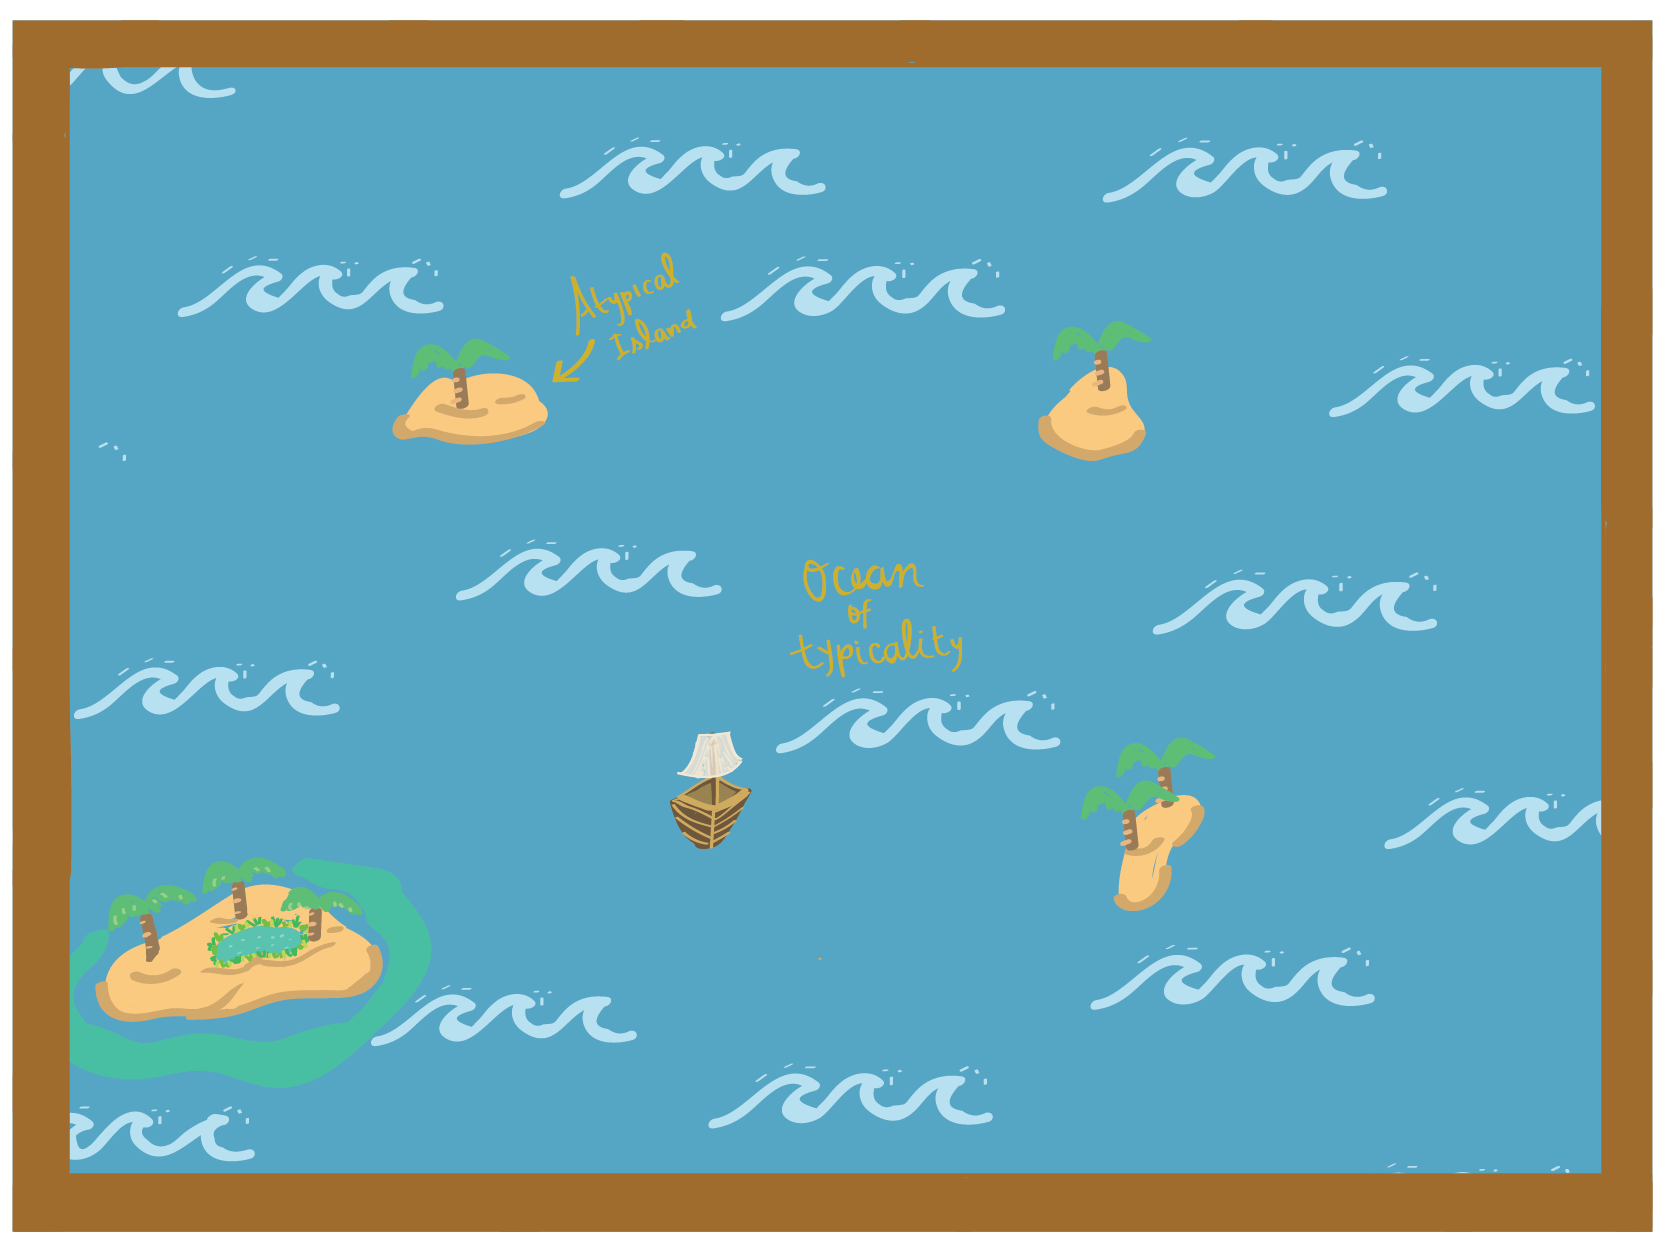
\includegraphics[width=0.9\textwidth]{Figures/ocean-of-typicality.png}
%\caption{Illustration of the canonical typicality in a map chart. The boat here refers to a random picked state in our universe, and the islands refer to those states who radically differ from the Canonical state.}
%\label{figura_tipicidad}
%\end{figure}
\indent To formally express canonical typicality, it is necessary to first define a notion of distance between states $\rho_S$ and $\Omega_S$, as well as a measure over which pure states $\ket{\phi}$ are defined.\\
\indent We define the trace distance between $\rho_S$ and the canonical state $\Omega_S$, by  $||\rho_S-\Omega||_1$, this distance is explicitly calculated by
\begin{equation}
||\rho||_1=\operatorname{Tr}|\rho|=\operatorname{Tr}\left(\sqrt{\rho^{\dagger} \rho}\right).
\label{CH1:Trace_distance}
\end{equation}
Consider $\ket{\phi}$ to be a pure state in $\mathcal{H}_R$, with respective dimension $d_R$. As the state is normalized ($\langle\phi | \phi\rangle=1$) we know that the pure state $\ket{\phi}$ lives in a ($2d_R-1$)-dimensional real sphere. Thus, the states the state $\ket{\phi}$ lives over the sphere surface of $d_R$ dimensions. Hence, if we are randomly sample pure states, we will have to sample them with the previously discussed Haar measure, which is the measure that is invariant under unitary transformations.\\
Therefore the theorem of canonical typicality reads,
% clarified the Now with the notion of the distance we chose to work with, and the space where these pure states live in, we are ready to announce the general result in typicality.\\
\begin{theorem}[Theorem of Canonical Typicality \cite{popescu_entanglement_2006,popescu_foundations_2005}.]
For a random chosen state, sampled with the Haar measure, $\ket{\phi}\in\mathcal{H}_R\subset\mathcal{H}_S\otimes\mathcal{H}_B$ and arbitrary $\varepsilon >0$ the distance between the reduced density matrix $\rho_{S}=\operatorname{Tr}_{E}(|\phi\rangle\langle\phi|)$ and the canonical state $\Omega_S=\operatorname{Tr}_E\mathcal{E}_R$ is given probabilistically by:
\begin{equation}
\operatorname{Prob}\left(\left\|\rho_{S}-\Omega_{S}\right\|_{1} \geq \eta\right) \leq \eta^{\prime},
\label{CH1:Typicality_result_1}
\end{equation}
where
\begin{equation}
\eta=\varepsilon+\sqrt{\frac{d_{S}}{d_{E}^{\mathrm{eff}}}}, \quad \eta^{\prime}=2 \exp \left(-C d_{R} \varepsilon^{2}\right),
\label{CH1:Typicality_result_1_1}
\end{equation}
with
\begin{equation}
C=\frac{1}{18 \pi^{3}}, \quad d_{E}^{\mathrm{eff}}=\frac{1}{\operatorname{Tr} \Omega_{E}^{2}}\geq \frac{d_R}{d_S}, \quad \Omega_{E}=\operatorname{Tr}_{S} \mathcal{E}_{R}
\label{CH1:Typicality_result_1_2}
\end{equation}
\end{theorem}

Note that $\eta$ and $\eta'$ are small quantities, thus, we can assert that whenever $d^{\mathrm{eff}}_E\ggg d_S$ and $d_R\varepsilon^2\ggg 1$, every reduced state will be close to its correspondent canonical state. What this results tells us is that probabilistically speaking, if the dimension of the accessible space ($d_R$) is large enough, we will have that for the overwhelming majority of choices of random pure states, will have almost certainly that every subsystem, with small enough dimension, will be indistinguishable from the canonical state. Moreover, Popescu et. al \cite{popescu_entanglement_2006} find an bound to the average differences between the state of the system (the reduced state) and the canonical state. Explicitly, using the levy lemma, they are able to show 

\begin{equation}
\left\langle\left\|\rho_{S}-\Omega_{S}\right\|_{1}\right\rangle \leq \sqrt{\frac{d_S}{d_E^{\mathrm{eff}}}}\leq\sqrt{\frac{d_{S}^{2}}{d_{R}}}.
\label{CH1:Typicality_result_2}
\end{equation}

This bound tells us that most of pure states constraint to a global restriction have the property that when we look at the local state of the system it seem to behave as the thermal state. This result is what motivated the illustration shown in \ref{figura_tipicidad}.\\
\indent In despite this result explains very well the reason why by randomly choosing a state $\ket{\phi}$ over the Haar measure, it coincides with the canonical state in almost all cases, it does not explain the way a state out of equilibrium (atypical state), reaches equilibrium. An the reason for that is that no particular evolution was considered here, and only probabilistic arguments were used. this means that typicality is a kinematic description of thermalisation. However, because almost all states of the universe have the property that the system is in a approximately at the canonical state, we anticipate that most evolutions will quickly carry a state in which the system is not thermalised to one in which it is. Namely, in the next section we will see how from a typicality viewpoint,  Linden et. al.\cite{linden_quantum_2009} were able to show that thermalisation can occur in a system reliant on a unitary dynamic.

\section{Evolution Towards Equilibrium.}

Typicality is kinematic result, meaning that is only valid for a given time and a given state, and were unitary evolution does not play a role. Specifically, we are interested in states that are atypical, in the sense that are states that locally drastically from the canonical state. As pointed out by Linden et. al.\cite{linden_quantum_2009}, to prove thermalisation is a much complicated problem since a closer look of the elements present in thermalisation, shows that equilibration, environment state independence, system state independence and the Boltzmannian form of the state of equilibrium are needed to assure that thermalisation has taken place. Specifically, the result obtained by Linden et. al. in \cite{linden_quantum_2009} addressed only the first two elements, showing that, equilibrium can be understood as a local universal property of Quantum systems. It is important to stress that when we refer to equilibrium we do not necessarily refer to thermal equilibrium; indeed the equilibrium state can be an arbitrary state with only the property that it does not change over time.\\
\indent To understand how is possible to prove that equilibrium appear as a ``typical behaviour'' in quantum mechanics. It is important to first define some concepts that we have used before but that we consider are important to make explicit.\\


\begin{definition}[Universe, system and environment:] For us the universe will refer always to a large quantum system living in a Hilbert space $\mathcal{H}$. As before, our universe is always decomposed in two,  and in this decomposition we refer to the system $S$ as a small part of the total Hilbert space. The remaining, we will call it the environment. Explicitly we will always decompose the Hilbert space of the universe as a tensor product of the Hilbert space of the system and the environment, $\mathcal{H}=\mathcal{H}_S\otimes \mathcal{H}_E$, where $d_S$ and $d_E$ are the respective dimension of the system and the environment. 
\end{definition}
Note that  the environment nor the system have been provided with any special property, meaning that for this formulation, the system could be a single particle or even a section of a lattice.\\
\indent For the sake of proving the result in \cite{linden_quantum_2009}, we also define the Hamiltonian of the universe as
\begin{definition}[Hamiltonian:]
The evolution of the universe will be governed by a Hamiltonian given by
\begin{equation}
\hat{H}=\sum_{k}E_k\ket{E_k}\bra{E_k}.
\label{CH1:Hamiltonian_universe_linden}
\end{equation}
with $\ket{E_k}$ the eigenstate in the energy basis with energy $E_k$. Where the main required assumption is that the Hamiltonian has non-degenerate energy gaps.
\end{definition}
%related with the possible values of energies this Hamiltonian can have. The only requirement needed the Hamiltonian to have non-degenerate energy gaps.
Expressing this condition in a more  explicit way, it is said that a Hamiltonian has no-degenerate energy gaps if any non-zero difference of eigenvalues of energy determine the two energy values involved. That is, for any four eigenstates with energy $E_k$, $E_\ell$, $E_m$, $E_n$, satisfy that if $E_{k}-E_{\ell}=E_{m}-E_{n}$, then $m=n$ and $k=\ell$, or $k=m$ and $\ell = n$. \\
\indent Notice that the restriction imposed to the Hamiltonian is an extremely natural constraint, because all Hamiltonians that lack of symmetries have non-degenerate energies, so we talk about a set of Hamiltonians with measure $1$ that fulfils this condition.\\
\begin{definition}[Notation:]
We will work here with pure time dependent states of the universe, states that will be represented by $\ket{\Psi(t)}$ with a time dependent density matrix given by $\rho(r) =\ket{\Psi(t)}\bra{\Psi(t)}$. 
\end{definition}
Thus the state of the system at a time $t$ can be found by tracing out the environment, that is, $\rho_S(t)=\operatorname{Tr}_E \rho(t)$, and identically, we define the state of the environment as $\rho_E(t)=\operatorname{Tr}_S \rho(t)$.\\
\indent It is convenient to define the transient states of the universe, or the time averaged state $\omega$ as
\begin{equation}
\omega=\langle\rho(t)\rangle_{t}=\lim _{\tau \rightarrow \infty} \frac{1}{\tau} \int_{0}^{\tau} \rho(t) d t.
\label{CH1:average_time_state}
\end{equation}
This definition allows us to also define $\omega_s$ and $\omega_E$ as the time averaged state of the system and the environment respectively. Finally, we re introduce the concept of the effective dimension of a mixed state $\rho$:
\begin{equation}
d^{\mathrm{eff}}(\rho)=\frac{1}{\operatorname{Tr}\left(\rho^{2}\right)}.
\label{CH1:Effective_dimension}
\end{equation}
The meaning of this effective is how many states contribute to the mixture, carrying the probabilistic weight of different states in the mixture, and different than the support of an operator in the Hilbert space, it is a continuous measure.\\
\indent With the concepts aforementioned, Linden et. al.  \cite{linden_quantum_2009} are able to show that every pure state of a quantum universe, composed by a large number of eigenstates of energy, and that evolves under an arbitrary Hamiltonian, is such that every small system will equilibrate. where the reason of consider the global state to have many eigenstates of energy is because fi there are many eigenstates, we can assure that there will be a large quantity of changes throughout the evolution of the system. The notion of evolving through many states can be mathematically encapsulated via the effective dimension of the time average state $\omega=\langle\rho(t)\rangle_{t}$, and the connection between this and the number of eigenstates is with ease seen by expanding $\ket{Psi(t)}$ as

%\footnote{The reason why we need the global state to have many eigenstates of energy is because by imposing this we can assure that there will be a large quantity of changes throughout the evolution of the system.}
%\indent Where the reason of requiring the universe to have many changes in its time evolution, is because for equilibration to take place it is needed that part of the information of the initial state of the system leaves the system and enters in the environment. This notion of evolving through many states can be mathematically encapsulated via the effective dimension of the time average state $\omega=\langle\rho(t)\rangle_{t}$, and the connection between this and the number of eigenstates is with ease seen by expanding $\ket{Psi(t)}$ as
\begin{equation}
|\Psi(t)\rangle=\sum_{k} c_{k} e^{-i E_{k} t}\left|E_{k}\right\rangle
\label{CH1:expansion_1}
\end{equation}
where $\sum_{k}\left|c_{k}\right|^{2}=1$ and hence
\begin{equation}
\rho(t)=\sum_{k, l} c_{k} c_{l}^{*} e^{-i\left(E_{k}-E_{l}\right) t}\left|E_{k}\right\rangle\left\langle E_{l}\right|,
\label{CH1:expansion_2}
\end{equation}
that can be expanded and written as
\begin{equation}
\begin{aligned}
\rho(t)=\underbrace{\sum_{n}\|c_{n}\|^{2}\ket{E_{n}}\bra{E_{n}}}_{\omega}&+\underbrace{\sum_{m \neq n} c_{n} c_{m}^{*}\ket{E_{n}}\bra{E_{m}} e^{-i t\left(E_{n}-E_{m}\right)}}_{\lambda (t)} \\
&=\omega+\lambda(t).
\end{aligned}
\label{CH1:Expansion_to_use_after}
\end{equation}
For the case of non-degeneracy of the energy levels, we have that the cross-terms vanish, that is
\begin{equation}
\omega=\langle\rho(t)\rangle_{t}=\sum_{k}\left|c_{k}\right|^{2}\left|E_{k}\right\rangle\left\langle E_{k}\right|,
\label{CH1:expansion_3}
\end{equation}
which will lead us to 
\begin{equation}
d^{\mathrm{eff}}(\omega)=\frac{1}{\operatorname{Tr}\left(\omega^{2}\right)}=\frac{1}{\sum_{k}\left|c_{k}\right|^{4}}.
\label{CH1:expansion_4}
\end{equation}
In the same way as in typicality, we are going to ask ourselves about the distance between $\rho_{S}(t)$ and $\omega_{S}=\left\langle\rho_{S}(t)\right\rangle_{t}$. To do this, we first compute the difference between $\rho_S(t)$ and $\omega_{S}$ in terms of the energy eigenstates as
%where $D$ will refer to the trace distance we already discussed.
%\footnote{Here has in the case of typicality we use the trace distance.}, 
\begin{equation}
\rho_{S}(t)-\omega_{S}=\sum_{m \neq n} c_{m} c_{n}^{*} e^{-i\left(E_{m}-E_{n}\right) t} \operatorname{Tr}_{E}\left|E_{m}\right\rangle\left\langle E_{n}\right|.
\label{CH1:expansion_5}
\end{equation}
Since in general we know that $\rho_S(t)$ fluctuates around the state $\omega_S$, it is evident that the distance between them will change over time. Thus, we will be interested in the time average of the trace distance $\langle ||\rho_{S}(t), \omega_{S}||_1\rangle_t$. The value this average takes will tell us about where the system is spending most of its time. In other words $\langle ||\rho_{S}(t), \omega_{S}||_1\rangle_t$ will be small when the system equilibrates to $\omega_S$. To be able to prove what is announced as the \textit{Theorem 1} in \cite{linden_quantum_2009} it is useful to relate the trace distance to the square of the Hilbert-Schmidt distance using a standard bound provided in \cite{fuchs_cryptographic_1999}
\begin{equation}
||\rho_{1}-\rho_{2}||_1=\frac{1}{2} \operatorname{Tr}_{S} \sqrt{\left(\rho_{1}-\rho_{2}\right)^{2}} \leq \frac{1}{2} \sqrt{d_{S} \operatorname{Tr}_{S}\left(\rho_{1}-\rho_{2}\right)^{2}}.
\label{CH1:Linden_proof_1}
\end{equation}
Which combined with the concavity of the square-root function, yields
\begin{equation}
\left\langle ||\rho_{S}(t), \omega_{S}||_1\right\rangle_{t} \leq \sqrt{d_{S}\left\langle\operatorname{Tr}_{S}\left[\rho_{S}(t)-\omega_{S}\right]^{2}\right\rangle_{t}},
\label{CH1:Linden_proof_2}
\end{equation}
that provides us the bound we need to proof the theorem. Now using \eqref{CH1:expansion_5} we write
\begin{equation}
\left\langle\operatorname{Tr}_{\mathcal{S}}\left[\rho_{\mathcal{S}}(t)-\omega_{\mathcal{S}}\right]^{2}\right\rangle_{t}=\sum_{m \neq n} \sum_{k \neq l} \mathcal{T}_{k l m n} \operatorname{Tr}_{\mathcal{S}}\left(\operatorname{Tr}_{E}\left|E_{k}\right\rangle\left\langle E_{l}\left|\operatorname{Tr}_{E}\right| E_{m}\right\rangle\left\langle E_{n}\right|\right),
\end{equation}
where $\mathcal{T}_{k l m n}=c_{k} c_{l}^{*} c_{m} c_{n}^{*} e^{-i\left(E_{k}-E_{l}+E_{m}-E_{n}\right) t}$. We compute the time average taking into account that the Hamiltonian has non-degenerate energy gaps, thus, we find that
%\footnote{This condition is reflected in the evaluation by considering the terms where $k\neq\ell$ and $m\neq n$, leading to $m=\ell$ and $k=n$ are the only terms that contribute.} 

\begin{equation}
\begin{aligned}
\left\langle\operatorname{Tr}_{S}\left[\rho_{S}(t)-\omega_{S}\right]^{2}\right\rangle_{t} &=\sum_{k \neq l}\left|c_{k}\right|^{2}\left|c_{l}\right|^{2} \operatorname{Tr}_{S}\left(\operatorname{Tr}_{E}\left|E_{k}\right\rangle\left\langle E_{l}\left|\operatorname{Tr}_{E}\right| E_{l}\right\rangle\left\langle E_{k}\right|\right) \\
&=\sum_{k \neq l}\left|c_{k}\right|^{2}\left|c_{l}\right|^{2} \sum_{s s^{\prime} b b^{\prime}}\left\langle s b | E_{k}\right\rangle\left\langle E_{l} | s^{\prime} b\right\rangle\left\langle s^{\prime} b^{\prime} | E_{l}\right\rangle\left\langle E_{k} | s b^{\prime}\right\rangle\\
&=\sum_{k \neq l}\left|c_{k}\right|^{2}\left|c_{l}\right|^{2} \sum_{s s^{\prime} b b^{\prime}}\left\langle s b | E_{k}\right\rangle\left\langle E_{k} | s b^{\prime}\right\rangle\left\langle s^{\prime} b^{\prime} | E_{l}\right\rangle\left\langle E_{l} | s^{\prime} b\right\rangle \\
&=\sum_{k \neq l}\left|c_{k}\right|^{2}\left|c_{l}\right|^{2} \operatorname{Tr}_{E}\left(\operatorname{Tr}_{S}\left|E_{k}\right\rangle\left\langle E_{k}\left|\operatorname{Tr}_{S}\right| E_{l}\right\rangle\left\langle E_{l}\right|\right)\\
&=\sum_{k \neq l} \operatorname{Tr}_{E}\left[\operatorname{Tr}_{S}\left(\left|c_{k}\right|^{2}\left|E_{k}\right\rangle\left\langle E_{k}\right|\right) \operatorname{Tr}_{S}\left(\left|c_{l}\right|^{2}\left|E_{l}\right\rangle\left\langle E_{l}\right|\right)\right] \\
&=\operatorname{Tr}_{E} \omega_{E}^{2}-\sum_{k}\left|c_{k}\right|^{4} \operatorname{Tr}_{S}\left[\left(\operatorname{Tr}_{E}\left|E_{k}\right\rangle\left\langle E_{k}\right|\right)^{2}\right] \\
&\leq \operatorname{Tr}_{E} \omega_{E}^{2},
\end{aligned}
\label{CH1:Linden_proof_3}
\end{equation}
where $\omega_E=\operatorname{Tr}_S \omega$. To obtain a further bound, we invoke weak sub-additivity of the Re\'enyi entropy \cite{camilo_strong_2019}
\begin{equation}
\operatorname{Tr}\left(\omega^{2}\right) \geq \frac{\operatorname{Tr}_{E}\left(\omega_{E}^{2}\right)}{\operatorname{rank}\left(\rho_{S}\right)} \geq \frac{\operatorname{Tr}_{E}\left(\omega_{E}^{2}\right)}{d_{S}}.
\label{CH1:Linden_proof_4}
\end{equation}
Hence, combining \eqref{CH1:Linden_proof_2}, \eqref{CH1:Linden_proof_3} and \eqref{CH1:Linden_proof_4} we get
\begin{equation}
\left\langle ||\rho_{S}(t), \omega_{S}||_1\right\rangle_{t} \leq \frac{1}{2} \sqrt{d_{S} \operatorname{Tr}_{E}\left(\omega_{E}^{2}\right)} \leq \frac{1}{2} \sqrt{d_{S}^{2} \operatorname{Tr}\left(\omega^{2}\right)}.
\label{CH1:Inequality_last}
\end{equation}
By taking the definition of effective dimension, we get the main result shown in \cite{linden_quantum_2009}
\begin{equation}
\left\langle ||\rho_{S}(t), \omega_{S}||_1\right\rangle_{t} \leq \frac{1}{2} \sqrt{\frac{d_{S}}{d^{\mathrm{eff}}\left(\omega_{E}\right)}} \leq \frac{1}{2} \sqrt{\frac{d_{S}^{2}}{d^{\mathrm{eff}}(\omega) }}.
\label{CH1:Result_linden}
\end{equation}
As we can see, the result obtained by Linden et. al. tell us that the vast majority of quantum systems, in which the dynamic of the universe is governed by a Hamiltonian with no gaps, will spend most of its time close to its equilibrium state independently of its initial state. Note that this result is not necessarily considering that the state of equilibration will coincide with the canonical state, but since we expect to have thermal typicality in the system, that state of equilibrium will coincide with the thermal equilibrium.
\section{Consequences of typicality}
We presented typicality as an alternative mechanism to understand thermalisation in large quantum systems, and we saw how these ideas let us explain equilibration in large quantum systems. The purpose of this section will be to point some of the consequences within typicality.\\
\indent Consider two different orthogonal pure states living in the same Hilbert space ($\ket{E_n},\ket{E_m} \in \mathcal{H}_{R}$), the Hilbert space associated with the global restriction $R$. From typicality, we know that the each of the reduced states of $\ket{E_n},\ket{E_m}$ approximately leads to the canonical state, that is
\begin{equation}
\operatorname{Tr}_{\mathcal{E}} \ket{E_n}\bra{E_n} \approx \operatorname{Tr}_{\mathcal{E}} \ket{E_m}\bra{E_m} \approx \Omega_{\mathcal{S}}.
\end{equation}
Consider a third state $\ket{\Psi}$ to be a generic linear combination of $\ket{E_n}$ and $\ket{E_m}$, fulfilling the same restriction $R$ of the universe. In this case we will have that the density matrix associated with the third state is
\begin{equation}
\begin{aligned}
\rho &= \ket{\Psi}\bra{\Psi}\\
&= \|c_n\|^2 \ket{E_n}\bra{E_n} +  \|c_m\|^2 \ket{E_m}\bra{E_m} \\
& + c_n c^{*}_m  \ket{E_n}\bra{E_m}+ c_m c^{*}_n \ket{E_m}\bra{E_n}.
\end{aligned}
\label{CH1:State_as_function_of_time}
\end{equation}
If we take the partial trace of the equation \eqref{CH1:State_as_function_of_time}, we will end up with the state of the system,
\begin{equation}
\begin{aligned}
\rho_S &= \operatorname{Tr}_E \rho = \operatorname{Tr}_E  \ket{\Psi}\bra{\Psi}\\
&= \|c_n\|^2\operatorname{Tr}_E  \ket{E_n}\bra{E_n} +  \|c_m\|^2 \operatorname{Tr}_E \ket{E_m}\bra{E_m} \\
& + c_n c^{*}_m  \operatorname{Tr}_E \ket{E_n}\bra{E_m} + c_m c^{*}_n \operatorname{Tr}_E \ket{E_m}\bra{E_n}.
\end{aligned}
\label{CH1:State_as_function_of_time_system}
\end{equation}
\indent  Notice that the way we constructed the state $\ket{\Psi}$, makes the non-crossed terms in \eqref{CH1:State_as_function_of_time_system} to approximately  coincide with $\operatorname{Tr}_E \ket{E_n}\bra{E_n} =\operatorname{Tr}_E \ket{E_m}\bra{E_m} \approx \Omega(E)$, with $\Omega(E)$ the canonical state. Thus, the equation \eqref{CH1:State_as_function_of_time_system} can be written as
\begin{equation}
\rho_S= \Omega(E) + c_n c^{*}_m  \operatorname{Tr}_E \ket{E_n}\bra{E_m} + c_m c^{*}_n \operatorname{Tr}_E \ket{E_m}\bra{E_n}.
\label{CH1:State_as_function_of_time_system_typicality}
\end{equation}
In order to get the equality, the cross terms in \eqref{CH1:State_as_function_of_time_system_typicality} have to  approximately vanish. This property of vanishing partial traces of exterior products of states is what we name \textit{ultra-orthogonality}. Explicitly, that is,
\begin{equation}
\operatorname{Tr}_E \ket{E_n}\bra{E_m} = \operatorname{Tr}_E \ket{E_m}\bra{E_n} \approx  0.
\label{CH1:Property_of_super_orthogonality}
\end{equation}
Notice that this property appears naturally by just using the results of typicality, and more importantly, the property of getting vanishing partial traces over the crossed terms could explain the path to equilibrium as an instant process. To see this, we can replace the condition \eqref{CH1:Property_of_super_orthogonality} in equation \eqref{CH1:expansion_5} and see that
\begin{equation}
\operatorname{Tr}_{\mathcal{E}}\rho(t)\equiv \rho_{\mathcal{S}} \approx \omega_{\mathcal{S}}.
\label{CH1:inst_eq}
\end{equation}
Notice that whenever ultra-orthogonality holds, temporal averages are not needed and equilibration will appear as an instantaneous process. Inspired on this interesting phenomena, we decided to explore ultra-orthogonality for the special case in which the terms in \eqref{CH1:Property_of_super_orthogonality} of the left hand side are exactly equal to zero, and thus implying the equality in equation \eqref{CH1:inst_eq}. This means that the correspondent reduced state of a fully interacting universe will be immediately constant. The idea of this work is to explore if it is possible to find Hilbert spaces in which ultra-orthogonality holds, and more importantly, to find out how big these Hilbert spaces can be.\\
\indent Specifically we will be interested in the question ``what is the biggest Hilbert space in which ultra-orthogonality will holds?''. In the next chapters we will  answer this question for the specific case of systems that can be mapped to fermionc systems through non-local transformations. % that are like the reduce our problem to Fermionic systems and we will show that for this specific case, we are able to find exponentially large Hilbert spaces where ultra-orthogonality holds.
%which tell us that these crossed terms should be of the order of the fluctuations in the system, because dimension generally grows exponentially with the number of particles, we would expect any fixed power of $d_{S}$ to be much smaller than than $d^{\operatorname{eff}(\omega_E)}$. Considering this, we state that an alternative mechanism which makes the systems to equilibrate emerge naturally as a consequence of typicality.\\

%Inspired on this, we decided to explore ultra-orthogonality for the special case in which the terms in \eqref{CH1:Property_of_super_orthogonality} of the left hand side are equal to zero, strictly speaking. What this implies is that whenever we look at the reduced state of this universe, it will be immediately stationary, that is


%and to show that for that special case, thanks to an alternative interpretation of Fermionic states, we are able to find exponentially large Hilbert spaces where ultra-orthogonality holds.
% \footnote{Note that we are not expecting to stumble upon the thermal state, this result only tell us about the correspondent state of equilibrium for the reduced state. Nonetheless, since thermal typicality is expected on the system, one might think that this equilibrium state correspond to the canonical one. }.
% Up to this point, one might think that this condition is quite restrictive and that just few states will satisfy it. We are going to provide arguments to show that it is not the case in Fermions, and that indeed there is an exponentially large Hilbert subspace of states fulfilling this condition. More over we will show how this is possible to prove by using tools taken from Fermionic random minimum codes.

% a physical system such that can be solved analytically (or numerically). Take into account that the latter requirement is needed to have a complete knowledge of the state of our universe, and be able to then take a small portion of it to study this reduced state. Thus in order to do that, it is necessary to be able to compute with relative easiness the diagonalization of our universe as well as the reduced states of it in an efficient way\footnote{We emphasise that it has to be efficient because the trend of exponential growth inherit by Hilbert spaces turns out to be a challenging problem when working with large systems.}. In the following sections we will provide the background required to understand the choice of the system we made as well as a detailed calculations which provide a full characterization of this system and its reduced states. More over we show a way to generalise this result to any Fermionic system and how this ultra-orthogonality is related with a minimal distance code.
\chapter{Quantum Trajectories.}
Often when we refer to trajectories the idea of a path comes into our minds which often is continuous in time, nevertheless, this idea is not always correct when we talk about quantum systems,  but we can keep the essence of the idea to interpret that for quantum systems a trajectory will be like the path taken by a conditional state for which the unconditional system state evolves continuously\footnote{The concept of conditional state of a system, is also know as the a-posteriori state, and it's basically the state found by using Bayesian inference. Therefore, one can infers what is happening in the system by using the readout, and is based on Bayes' theorem. From this theorem it is possible to derive that the conditional system state is given by
\[P_{X,Y}'(x|y)=\frac{P_{X,Y}(y|x)P_{X}(x)}{P_{Y}(y)}=\frac{P_{X,Y}(y|x)P_{X}(x)}{\sum_{x}P_{X,Y}(y|x)P_{X}(x)},\]
and we can also define an unconditional state by averaging over the possible measurement results as
\[P_{X}'(x)=\sum_{y}P_{X,Y}'(x|y)P_{Y}(y),\]
here the random variables $X$ and $Y$ represent the system state and the output respectevely(see the first section of \cite{Wiseman}).}.\\
The concept of quantum trajectories has provoked a huge activity in the community of quantum optics in the last years. From all this activity there has been three different interpretations of quantum trajectories: Not real, subjectively real and objectively real\cite{Wisemantrajectories}.
\subsection*{Non-Real Quantum Trajectories}
The interpretation of these ``non-real'' quantum trajectories is just simply that this formalism is just a numerical tool for solving the master equation, because computationally speaking, to solve these equations we only need $2N-2$ real numbers that have to be stored in an $N$-dimensional Hilbert space, compared to $N^{2}-1$ numbers for a state matrix.
\subsection*{Subjectively Real Quantum Trajectories}
This interpretation consider sort of degree of reality at the quantum trajectories, and the name of ``subjective reality'' s because the nature of these trajectories depend on the scheme that the observer has chosen to measure. Therefore, once the procedure of measurement has been chosen the time evolution of the conditioned system is real in the sense that for every observer the results will be the same. The subjectivity comes when we want to make an statement over a system, like for example ``an isolated exited atom will spontaneously decay at a random time'', this is not possible unless we place a photodetector to detect the emitted photon. In the case of a different procedure of measurement like heterodyne detection, we will register a continuous flow of radiation from the atom instead of a jump. Hence, the stochastic evolution of the system becomes real when the system is subject to an observation, and it is not real in an observer-less universe. 
The work done by Carmichael and co-workers \cite{Carmichaelquantum,PhysRevLett.70.2273,PhysRevLett.75.45,PhysRevA.46.R6801,Carmichael1994} was made by the motivation of the computational advantage and even though, most of their work is numerically it was possible to obtain son analytic results for son particular schemes of measurement and particular systems. There are some reasons to consider the measurement interpretation of quantum trajectories, and some of them are basically that these have opened the possibility for solve partially analytically measurement theory problems, and that subjectively real quantum trajectories give a different understanding of irreversible processes than the ones that master equation gives us.
\subsection*{Objectively Real Quantum Trajectories}
The last interpretation over quantum trajectories, consider these trajectories as independent of the measurement scheme, and this interpretation is based on the distrust of the standard interpretation of quantum mechanics, and a target to replace subjective collapses due to measurements with ``objectively real collapses'', and the roots of these approach date back to the original interpretation of the wave-function proposed by Schr\"odinger, which tries to give a real meaning of the wave-function, these interpretations are similiar to the Bohomians\cite{PratimKumar} trajectories in which the theory itself is a theory of hidden variables, which the wave-function has a representation of reality, having meaning only when irreversible processes occur. The basic problem with this ``objective'' interpretation lies with the origin of irreversible evolution. For example in optics, the master equation can be regarded as an approximation to the exact reversible evolution for the system plus its environment just as we showed in the chapter \ref{openquantumsystems}, then the problem with this interpretation is that all authors that have boarded this interpretation have not found an explanation for what is meant to be truly irreversible and what is not.\\

Here we are going to use the interpretation of ``Subjectively Real Quantum trajectories''  to describe a quantum measurement theory just as is proposed by Wiseman and Carmichael. By this approach it is possible to recreate Lindblad's equation by the simplest sort of quantum trajectories which involves a discontinuous conditioned evolution. 
\section{Continuous measurements.}
There are different approaches to describe continuous quantum measurements such as:
\begin{itemize}
\item Models of measurement.
\item Master equation
\item restricted path integrals
\item Stochastic Schr\"odinger eqution
\end{itemize}
Apart from the first one, all these ways of description are phenomenological. The conceptually most simple phenomenological approach is based upon the master equation for the density matrix, therefore, here we are going to use the ``Stochastic Scr\"odinger equation'' approach to describe continuous measurements\cite{jurgen}.\\
In order to generalise the unitary evolution of quantum states we incorporate an evolution conditioned to the measurements. Then we look for a differential equation for the density matrix state rather than the state. If we measure in an infinitesimal time, when a system it is being measured continuously (measurement time going to zero) we say that we are ``monitoring'' the system. Therefore, the evolution of the density matrix at time $t+dt$ can be obtained by averaging over all possible results
\begin{equation}
\rho(t+dt)=\sum_{r}\mathcal{J}[\hat{M}_{r}(dt)]\rho(t).
\label{quantumtrajectory1}
\end{equation}
If $\rho(t+dt)$ is differs in an infinitesimal quantity from $\rho(t)$ then we could think that at the time $dt$ we have obtained just one result ($r=0$) and set
\begin{equation}
\hat{M}_{r}(dt)=\hat{\mathbb{I}}-\left(\frac{\hat{\text{R}}}{2}+\frac{i}{\hbar}\hat{H}\right)dt,
\label{quantumtrajectory2}
\end{equation}
where $\hat{H}$ and $\hat{R}$ are Hermitian operators. However, the problem of just consider this result of measurement is that this measurement operator does not satisfy the completeness condition given in equation \eqref{Krauscompleteness} in the appendix \ref{superoperators}\footnote{As the measurement time is supposed to be infinitesimal we only preserve terms of order $dt$},
\[\hat{M}_{0}^{\dagger}(dt)\hat{M}_{0}(dt)=\hat{\mathbb{I}}-\hat{\text{R}}dt\neq \hat{\mathbb{I}}.\]
From the latter result we conclude that it's not possible to have only one measurement, because the measurement operator should be unitary\footnote{The condition of unitary is based on the fact that one can collect all information back if we would not have this condition there would be something lost and here we are assuming that everything can be recover when measured.} and as $\hat{R}\neq 0$ we need at least other possible result to fulfil the condition $\sum_r\hat{M}_r^{\dagger}(dt)\hat{M}_r(dt)$. the simplest suggestion is to consider a measurement such that $\hat{M}^{\dagger}_1(dt)\hat{M}_1(dt)=\hat{\text{R}}dt$,thus, we have that
\[\hat{M}^{\dagger}_0(dt)\hat{M}_0(dt)+\hat{M}^{\dagger}_1(dt)\hat{M}_1(dt)=\hat{\mathbb{I}},\]
which is what we wanted. Now we can consider that the possible results of measurements can be either $0$ or $1$, then we can write $\hat{\text{R}}$ and $\hat{M}_{1}(dt)$ explicitly as

\begin{align*}
\hat{M}_{1}(dt)&=\sqrt{dt}\hat{J},\\
\hat{\text{R}}&=\hat{J}^{\dagger}\hat{J},
\end{align*}
and from equation \eqref{quantumtrajectory1} we get that the evolution of $\rho$ is given by
\begin{equation}
\rho(t+dt)=\left[\hat{\mathbb{I}}-(\frac{\hat{J}^{\dagger}\hat{J}}{2}+\frac{i}{\hbar}\hat{H})dt\right]\rho(t)\left[\hat{\mathbb{I}}-(\frac{\hat{J}^{\dagger}\hat{J}}{2}-\frac{i}{\hbar}\hat{H})dt\right]+\hat{J}\rho(t)\hat{J}^{\dagger}dt,
\label{trajectory3}
\end{equation}
which has the differential form of Lindblad equation if we just take the terms of order $dt$
\begin{equation}
\dot{\rho}=-\frac{i}{\hbar}[\hat{H},\rho]+\hat{\mathcal{D}}[\hat{J}]\rho\equiv\mathcal{L}\rho.
\label{lindblad2}
\end{equation}
\section{Stochastic evolution}
As we consider above we can have two possible results of measurement $r=0,1$, then we can  compute the probability of having either $0$ or $1$ as
\[P_{1}(dt)=\text{tr}[\mathcal{J}[\hat{M}_1(dt)]\rho]=dt\text{tr}[\hat{J}^{\dagger}\hat{J}\rho],\]
\[P_{0}(dt)=1-P_1(dt).\]
Then the measurement with result $r=0$ it's considered as a null result, for this case we say that the system changes infinitesimally, but not unitarily, with the operator $\hat{M}_0(dt)$. At random times the result $r=1$ appears and this happen at rate $P_{1}(dt)/dt$ which is called a detection, and the evolution has an evolution given by the operator $\hat{M}_1(dt)$, this is what is known as a quantum jump. The interest of this case of ``quantum jumps'' is that any ``noisy trajectory'' (stochastic) can be approximate by quantum jumps.\footnote{The condition over these quantum jumps is that they have to range in size from being infinitesimal, this to guarantee that the state of the system after a jump will be always orthogonal to the one before the jump\cite{PhysRevLett.74.4827, Wiseman2002, 0305-4470-30-21-026, articlediosi}.} Nonetheless, it is important to emphasize that here this jumps represent a sudden change in the knowledge of the observer instead of an objective physical event as in Bohr's  original conception (Copenhagen interpretation)\cite{Bohr1913-BOHOTC}.\\
As we said, the evolution of the state is: either it jumps or it does not and it does it with a probability $P$ and $1-P$ respectively, this allow us then to write the evolution of the state as\footnote{See that it's necessary to normalize the state $\ket{\psi(t)}$ since we want the inner product to be orthonormal ($\bra{\psi(t)}\ket{\psi(t)}=1 \ \forall \ t$).}
\begin{equation}
\ket{\psi(t+dt)}=\left(
P\frac{\hat{M}_{1}(dt)}{\sqrt{\braket{\hat{M}_{1}^{\dagger}\hat{M}_{1}}(dt)}}+(1-P) \frac{\hat{M}_0(dt)}{\sqrt{\braket{\hat{M}_{0}^{\dagger}\hat{M}_{0}}(dt)}}\right)\ket{\psi(t)}.
\label{trajectory4}
\end{equation}
%We write it in this way in order to see that the evolution of the system can take one way  or another with probabilities $P$ and $1-P$ 
As we only have 2 possible outcomes $0$ and $1$, then the number of detections in function of time $N(t)$, then the stochastic increment $dN(t)$ must obey the following conditions\footnote{Here we are assuming that at time $t$ the state is a pure state, even though this could sound too ideal, a property of perfect monitoring is that if the system is initially in a pure state then, under perfect monitoring of its environment, this will remain in a pure state. Making then the system change its pure state in a stochastic and non-linear way.}
\begin{align}
dN(t)^{2}&=dN(t),\label{stochasticnumber}\\
\text{E}[dN(t)]&=\bra{\psi(t)}\hat{M}_{1}^{\dagger}(dt)\hat{M}_{1}(dt)\ket{\psi(t)}\equiv\braket{\hat{M}_{1}^{\dagger}(dt)\hat{M}_{1}(dt)}\nonumber\\
&=dt\bra{\psi(t)}\hat{J}^{\dagger}\hat{J}\ket{\psi(t)}dt\equiv dt\braket{\hat{J}^{\dagger}\hat{J}}(t)\label{expectedvaluedn}
\end{align} 
Let's compute now the expected value of $\hat{M}_0$\footnote{Here the expected value is the expected value over the ensemble or over the noise process.},
\[\bra{\psi(t)}\hat{M}_{0}^{\dagger}\hat{M}_{0}\ket{\psi(t)}\]

\[\bra{\psi(t)}\left(\hat{\mathbb{I}}-\frac{1}{2}\hat{J}^{\dagger}\hat{J}dt-\frac{i}{\hbar}\hat{H}dt\right)\left(\hat{\mathbb{I}}-\frac{1}{2}\hat{J}\hat{J}^{\dagger}dt+\frac{i}{\hbar}\hat{H}dt\right)\ket{\psi(t)}\]
\[\bra{\psi(t)}\hat{\mathbb{I}}-\frac{1}{2}\hat{J}dt-\frac{i}{\hbar}\hat{H}dt\hat{\mathbb{I}}-\frac{1}{2}\hat{J}dt+\frac{i}{\hbar}\hat{H}dt+O(dt^{2})\ket{\psi(t)}\]
\begin{equation}
=\bra{\psi(t)}\hat{\mathbb{I}}-\hat{J}^{\dagger}\hat{J}dt\ket{\psi(t)},
\label{expectedvaluem0}
\end{equation}
with the equation \eqref{expectedvaluem0} we can rewrite the evolution of the state $\ket{\psi}$ if the outcome is 0 as,
\begin{align}
\frac{\hat{M}_{0}(dt)}{\sqrt{\braket{\hat{M}_{0}^{\dagger}\hat{M}_{0}}(dt)}}&\approx\left(\hat{\mathbb{I}}-\frac{1}{2}\hat{J}^{\dagger}\hat{J}dt-\frac{i}{\hbar}\hat{H}dt\right)\left(1+\frac{1}{2}\braket{\hat{J}^{\dagger}\hat{J}}dt\right)\nonumber\\
&=\hat{\mathbb{I}}+\left(\frac{1}{2}\braket{\hat{J}^{\dagger}\hat{J}}-\frac{1}{2}\hat{J}^{\dagger}\hat{J}-\frac{i}{\hbar}\hat{H}\right)dt,
\label{trajectory5}
\end{align}
\begin{figure}[h!]
\centering
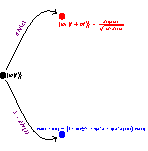
\includegraphics[width=0.7\textwidth]{Figures/equations.pdf}
\caption{Evolution of the system in the case of two possible measurements}
\label{Systemevolution}
\end{figure}  
which let us to write then the evolution of the state in terms of the stochastic differential $dN(t)$ as\footnote{Here we used the fact that $dN(t)dt$ is of higher order than $dt$ so this term can be neglect.}
\begin{align}
d\ket{\psi(t)}&=\left[\frac{\hat{M}_{1}(dt)}{\sqrt{\braket{\hat{M}_{1}^{\dagger}\hat{M}_{1}}(dt)}}-dN(t)\hat{\mathbb{I}}+\left(\frac{1}{2}\braket{\hat{J}^{\dagger}\hat{J}}-\frac{1}{2}\hat{J}^{\dagger}\hat{J}-\frac{i}{\hbar}\hat{H}\right)dt\right]\ket{\psi(t)}\nonumber\\
d\ket{\psi(t)}&=\left[\underbrace{dN(t)\left(\frac{\hat{M}_{1}(dt)}{\sqrt{\braket{\hat{M}_{1}^{\dagger}\hat{M}_{1}}(dt)}}-\hat{\mathbb{I}}\right)}_{\text{Stochastic part}}+\underbrace{dt\left(\frac{1}{2}\braket{\hat{J}^{\dagger}\hat{J}}-\frac{1}{2}\hat{J}^{\dagger}\hat{J}-\frac{i}{\hbar}\hat{H}\right)}_{\text{Deterministic part}}\right]\ket{\psi(t)}. 
\label{stochasticfashion}
\end{align}
Then as the equation \eqref{stochasticfashion} show us the evolution of the system can be expressed as one term which evolves in a deterministic way and another which give us the stochastic evolution of the system. The equation \eqref{stochasticfashion} is called stochastic mater equation and the solutions for these equations are called `\textit{Quantum trajectories} for the system.\\
In order to reconstruct the master equation, we consider a projector 
\[\hat{\Pi}(t)=\ket{\psi(t)}\bra{\psi(t)},\]
such that the expected value of this projector gives us the density matrix a time t
\begin{equation}
\text{E}[\hat{\Pi}(t)]\equiv\rho(t).
\label{projector}
\end{equation}
Just to simplify the notation we rewrite the equation \ref{stochasticfashion} as
\begin{equation}
\ket{d\psi(t)}=\ket{S(t)}dN+\ket{D(t)}dt,
\label{trajectory6}
\end{equation}
where $\ket{S(t)}$ and $\ket{D(t)}$ correspond to the stochastic and deterministic part respectively.
\[\ket{S(t)}=\left(\frac{\hat{M}_{1}(dt)}{\sqrt{\braket{\hat{M}_{1}^{\dagger}\hat{M}_{1}}(dt)}}-\hat{\mathbb{I}}\right)\ket{\psi(t)},\]
\[\ket{D(t)}=\left(\frac{1}{2}\braket{\hat{J}^{\dagger}\hat{J}}-\frac{1}{2}\hat{J}^{\dagger}\hat{J}-\frac{i}{\hbar}\hat{H}\right)\ket{\psi(t)}.\]
Then we take the differential of the projector $\hat{\Pi}(t)$and then we take the expected value and following the rules  \eqref{stochasticnumber} and \eqref{expectedvaluedn}  we derive an equation for $d\rho(t)$
\begin{align}
d\rho(t)&=\text{E}[d\hat{\Pi}(t)]=\text{E}\left[\ket{d\psi(t)}\bra{\psi(t)}+\ket{\psi(t)}\bra{d\psi(t)}+\ket{d\psi(t)}\bra{d\psi(t)}\right]\nonumber\\
&=\text{E}\left[\left(\ket{S(t)}dN+\ket{D(t)}dt\right)\bra{\psi(t)}+\ket{\psi(t)}\left(\bra{S(t)}dN+\bra{D(t)}dt\right)+\ket{S(t)}\bra{S(t)}dN\right]\nonumber\\
&=\text{E}\left[\left(\frac{\hat{J}\ket{\psi(t)}\bra{\psi(t)}\hat{J}^{\dagger}}{\braket{\hat{J}\hat{J}^{\dagger}}}-\ket{\psi(t)}\bra{\psi(t)}\right)dN+\left(\frac{i}{\hbar}\hat{H}\ket{\psi(t)}\bra{\psi(t)}-\frac{i}{\hbar}\ket{\psi(t)}\bra{\psi(t)}\hat{H}\right.\right.\nonumber\\
&\left.\left.-\frac{1}{2}\ket{\psi(t)}\bra{\psi(t)}\hat{J}^{\dagger}\hat{J}-\frac{1}{2}\hat{J}^{\dagger}\hat{J}\ket{\psi(t)}\bra{\psi(t)}+\braket{\hat{J}^{\dagger}\hat{J}}\ket{\psi(t)}\bra{\psi(t)}\right)dt\right]\nonumber\\
&=\text{E}\left[\left(\mathcal{G}[\hat{J}]dN(t)-dt\mathcal{H}\left[\frac{i}{\hbar}\hat{H}+\frac{1}{2}\hat{J}^{\dagger}\hat{J}\right]\right)\hat{\Pi}(t)\right],\label{trajectory7}
\end{align}
where the superoperators $\mathcal{G}$ and $\mathcal{H}$ are defined as
\begin{align}
\mathcal{G}[\hat{c}]\rho&=\frac{\hat{c}\rho\hat{c}^{\dagger}}{\text{tr}{\hat{c}\rho\hat{c}^{\dagger}}}-\rho, \label{superoperator1}\\
\mathcal{H}[\hat{c}]\rho&=\hat{c}\rho+\rho\hat{c}^{\dagger}-\text{tr}[\hat{c}\rho+\rho\hat{c}^{\dagger}]\rho. \label{superoperator2}
\end{align}
In order to compute the latter equation we have to use the property we have to generalise the equation \eqref{expectedvaluedn}, to calculate the expected value of the expression \eqref{trajectory7}, to do this we use a property of stochastic calculus which stablish that the way of compute an expected value of the product between a stochastic increment with expected value given by $\text{E}[dN(t)]=\lambda(X)dt$ and any function $g$ is
\begin{equation}
\text{E}[dN(t)g(\hat{\Pi}(t)]=dt\text{E}[\text{tr}[\hat{\Pi}\hat{J}^{\dagger}\hat{J}]g(\hat{\Pi}(t))],
\label{expectedvaluegeneral}
\end{equation}
then, combining the equations \eqref{trajectory7} and \eqref{expectedvaluegeneral} we get to a Lindblad's form of master equation given in \eqref{Lindbladeq}.
\begin{equation}
d\rho=-\frac{i}{\hbar}[\hat{H},\rho]dt+dt\mathcal{D}[\hat{J}]\rho.
\label{Lindbladeq2}
\end{equation}
By using the same  of argument equations \eqref{Lindbladeq2} and \eqref{stochasticfashion} can be generalised for more than just 2 possible outcomes and the these equations can be written as
\begin{equation}
\dot{\rho}=-\frac{i}{\hbar}[\hat{H},\rho]+\sum_{k}\mathcal{D}[\hat{J_{k}}]\rho,
\label{GeneralLindblad}
\end{equation}
\begin{equation}
d\ket{\psi(t)}=\sum_{k}\left[dN(t)\left(\frac{\hat{J}_{k}(dt)}{\sqrt{\braket{\hat{J}_{k}^{\dagger}\hat{J}_{k}}(dt)}}-\hat{\mathbb{I}}\right)+dt\left(\frac{1}{2}\braket{\hat{J}_{k}^{\dagger}\hat{J}_{k}}-\frac{1}{2}\hat{J}_{k}^{\dagger}\hat{J}_{k}-\frac{i}{\hbar}\hat{H}\right)\right]\ket{\psi(t)} ,
\label{Generaltrajectory}
\end{equation}
 
where $\hat{J}_{k}$ correspond to the the different operators that give the coupling between the bath and the system, these operators are also called Lindblad's operators\footnote{To check the different properties that these operators have see Appendix \ref{Lindbladappendix}.} \\


\section{Diffusive unravelings}

In every situation where a Markovian master equation can be derived, it is possible to continually measure the state of the environment, this happens if our measurements are made in a time scale large compared to the reservoir correlation time but small compared to the response time of the system.  this ``monitoring'' does not disrupt the system-reservoir coupling and the system will evolve according to the master equation, but an important situation that emerges from this is that first, the evolution of the system will follow the master equation if we ignore the results of the monitoring, however, if we take note of the results of monitoring the environment, the system will not longer obey the master equation\footnote{This is hard to understand, but as we saw in the foot note of the beginning of this chapter, if we ignore the results of the measurements we do not have knowledge certainty of the state and then we have to average over all possible outcomes whereas when we take note the uncertainty is nought since we know exactly what the state of the system is, this is the key to well understand when we refer to ``measuring ignoring the results'' and ``measuring reading the result'', and why these two have different evolution. }. 
To perfect ``monitoring'' of the environment some conditions have to be fulfilled, such as that all projective measurements have to be \textit{continual rank-one projective} well known as Von Neumann measurements or conventional measurements\footnote{Conventional measurements in quantum mechanics are defined as a collection of projector. Due to the  hermiticity of the observables, an observable $\hat{O}$ has a spectral decomposition $\hat{O}=\sum_{i}\lambda_{i}\hat{P}_{i}$ with $\hat{P}_{i}$ the projectors such that $\hat{P}_{i}\hat{P}_{j}=\hat{P}_{i}\delta_{ij}$, and $\lambda_{i}$ are unique. If $\hat{P}_{i}$ is not rank 1, it can be expressed as a sum of rank 1 projectors, this is, if the rank of $\hat{P}_{i}$ is $k$, 
\[\hat{P}_{i} =\hat{\Pi}_{1}+\hat{\Pi}_{2}+\ldots+\hat{\Pi}_{k},\]
where $\hat{\Pi}_{m}=\ket{\phi_{m}}\bra{\phi_{m}}$. Therefore, this means that projector with rank higher than 1 gives an uncertainty of the measurement since the result of the measurement will be a superposition of outcomes\cite{POVM1}\cite{POVM2}.}.
As we mentioned before the way to study quantum trajectories is via stochastic Schr\"odinger equation (SSE) which can be described as
\[\dot{\ket{\psi}}=-\frac{i}{\hbar}\hat{H}\ket{\psi}+ \text{noise}_{\psi}.\]
Although a SSE is conceptually the simplest way to define a quantum trajectory it results better if we use instead the stochastic master equation (SME), due to the invariance of the SME.\\
Assuming the initial state of the system to be pure, the quantum trajectory for its projector $\hat{\Pi}$ will be described by the SME of the form
\[\frac{d}{dt}\hat{\Pi}=\mathcal{L}\hat{\Pi}+\text{noise},\]
where the noise term is assuming to be diffusive and mean zero ($\braket{\text{noise}}=0$). By using the form of Îto calculus\footnote{A stochastic quantity $X(t)$ obeys an \^{I}to stochastic differential equation written as
\[dX=a[X(t),t)]dt+b[X(t),t]dW(t)],\]
if for all $t$ and $t_0$,
\[X(t)=X(t_0)\int_{t_{0}}^{t}dt'a[X(t'),t']+\int_{t_0}^{t}dW(t')b[X(t'),t'].\]
where $W(t)$ is a Wiener process, $X(t)$ is the variable of interest, $a[X(t),t]$ and $b[X(t),t]$ are certain known functions.\cite{StochasticNumerics}\cite{StochasticMethods}.} the latter equation can be written as
\begin{equation}
d\hat{\Pi}=\mathcal{L}\hat{\Pi}+dX,
\label{Itoform}
\end{equation}
where $dX$ is traceless, hermitian and depends linearly on the current pure state $\hat{\Pi}$ by simplicity we change $\hat{\Pi}$ by $\varrho$ to symbolise that the evolution of the projector is related with the evolution of the $\rho$ density matrix via the expected value.\\
As the SME is assumed to preserve the purity of the state the second moments of $\varrho$ are constrained by
\begin{equation}
\underbrace{d\varrho=d(\varrho^2)}_{\text{Pure state}}=\varrho d\varrho + d\varrho \varrho+d\varrho d\varrho =\underbrace{\{\varrho,d\varrho \}_{-}+d\varrho d\varrho}_{\text{Îto's calculus}},
\label{Itoscalculus}
\end{equation}
then from the equation \eqref{Itoscalculus} we see that the relation for pure states leads us to the differential relation given by Îto's calculus. This result must hold for arbitrary rank-one projectors (Von-Neumann).\\
Therefore, using Îto rules we get\footnote{In îto differentiation, one must keep all term up to second order in $dW(t)$ this means that for example if we want to compute the derivative of $\text{exp}(W(t))$ we have
\begin{align*}
d(\text{exp}(w(t))&=\text{exp}(W(t)+dW(t))-\text{exp}(W(t))=\text{exp}(W(t))\left(\text{exp}(dW(t))-1\right)\\
&=\text{exp}(W(t))\left(1+dW(t)+\frac{1}{2}dW^2(t)-1\right)=\text{exp}(W(t))\left(dW(t)+\frac{1}{2}dW^2(t)\right)
\end{align*}
It is possible to proof that $dW^2(t)=dt$ and $dW^{2+N}(t)=0$ $\forall \ N>0$.\cite{gardiner2004handbook}}
\[\mathcal{L}\varrho dt+dX=d\varrho=d(\varrho^2)=dt(\mathcal{L}\varrho)\varrho+dX\varrho+\varrho dt\mathcal{L}\varrho+\varrho dX+(dt\mathcal{L}\varrho+dX)(dt\mathcal{L}\varrho+dX)\]
\begin{equation}
=dt(\mathcal{L}\varrho)\varrho+dX\varrho+\varrho dt \mathcal{L}\varrho+\varrho dX+dXdX+dX dt\mathcal{L}\varrho+dt^2(\mathcal{L}\varrho)^2,
\label{Itolindblad1}
\end{equation}
as $dX\sim dt^{1/2}\Rightarrow dXdt\sim 0$ and $dt^2\sim 0$, then the equation \eqref{Itolindblad1} can be written as
\[dt\mathcal{L}\varrho+dX=dt\mathcal{L}\varrho \cdot\varrho+dX\varrho+\varrho dt \mathcal{L}\varrho+\varrho dX+dXdX,\]
by matching all the terms of order $dt$ and those of order $dX$,
\begin{equation}
dX=dX\varrho+\varrho dX=\{\varrho,dX\}_{+}
\label{Itolindblad2}
\end{equation}
\begin{align}
dt\mathcal{\varrho}=dt\mathcal{L}&\varrho \cdot\varrho+\varrho dt\mathcal{L}\varrho + dX dX,\nonumber\\
dXdX&=\mathcal{L}\varrho dt - dt\mathcal{L}\varrho\cdot \varrho - \varrho dt\mathcal{L}\varrho\nonumber\\
dXdX&=\mathcal{L}\varrho dt-\{\varrho,\mathcal{L}\varrho\}_{+}dt.\label{Itolindblad3}
\end{align}

A simple solution can be use as an ansatz to solve equation \eqref{Itolindblad2}
\begin{equation}
dX=\ket{d\varphi}\bra{\psi}+\ket{\psi}\bra{d\varphi}=\varrho dX+dX \varrho,
\label{ansatzitolindblad}
\end{equation}
where we have supposed that $\bra{d\varphi}\ket{\psi}=0$ and $\varrho=\ket{\psi}\bra{\psi}$, here $\ket{d\varphi}$ is an Îto differential of nought mean and is orthogonal to the current state $\ket{\psi}$.
Substituting \eqref{ansatzitolindblad} in \eqref{Itolindblad3}
\begin{align*}
&\left(\ket{d\varphi}\bra{\psi}+\ket{\psi}\bra{d\varphi}\right)\left(\ket{d\varphi}\bra{\psi}+\ket{\psi}\bra{d\varphi}\right)\\
&=\underbrace{\ket{d\varphi}\braket{\psi|d\varphi}\bra{\psi}}_{=0}+\ket{d\varphi}\underbrace{\braket{\psi|\psi}}_{=1}\bra{d\varphi}+\ket{\psi}\braket{d\varphi|d\varphi}\bra{\psi}+\underbrace{\ket{\psi}\braket{d\varphi|\psi}\bra{d\varphi}}_{=0},
\end{align*}
getting then an equation that $\ket{d\varphi}$ has to fulfil 
\begin{equation}
\ket{d\varphi}\bra{d\varphi}=\mathcal{L}\varrho dt-\{\varrho,\mathcal{L}\varrho\}_{+}dt-\ket{\psi}\braket{d\varphi|d\varphi}\bra{\psi}.
\end{equation}
To solve this equation we can use the orthogonality between the state $\ket{d\varphi}$ and $\bra{\psi}$. Multiplying by $\bra{\psi}\ldots\ket{\psi}$, it yields to
\[0=\bra{\psi}\mathcal{L}\varrho\ket{\psi}dt-\bra{\psi}\{\varrho,\mathcal{L}\varrho\}_{+}\ket{\psi}dt-\braket{d\varphi|\varphi}.\]
Expanding $\mathcal{L}\varrho$ given by equation \eqref{GeneralLindblad}, we get that the first term leads  us to
\[\bra{\psi}[\hat{H},\varrho]\ket{\psi}=\bra{\psi}\hat{H}\varrho-\varrho\hat{H}\ket{\psi}=\braket{\hat{H}}-\braket{\hat{H}}=0,\]
the second term
\begin{align*}
\bra{\psi}\hat{J}_k\varrho &\hat{J}_k^{\dagger}\ket{\psi}-\frac{1}{2}\bra{\psi}\hat{J}_k^{\dagger}\hat{J}_{k}\varrho+\varrho\hat{J}_k^{\dagger}\hat{J}_k\ket{\psi}\\
&=\braket{\hat{J}_k}\braket{\hat{J}_{k}^{\dagger}}-\frac{1}{2}\left(\braket{\hat{J}_k^{\dagger}}+\braket{\hat{J}_k^{\dagger}\hat{J}_k}\right)\\
&=\braket{\hat{J}_k}\braket{\hat{J}_{k}^{\dagger}}-\braket{\hat{J}_k^{\dagger}\hat{J}_k},
\end{align*}
Now looking at the term $\{\varrho,\mathcal{L}\varrho\}_{+}$, the part including the commutator gives us zero since $\varrho[\hat{H},\varrho]+[\hat{H},\varrho]\varrho=[\hat{H},\varrho]$, so, we look only at the other terms leading us to
\begin{align*}
\bra{\psi}\{\varrho,\mathcal{L}\varrho\}_{+}\ket{\psi}&=-\braket{\hat{J}_k^{\dagger}\hat{J}_k}-\frac{1}{2}\braket{\hat{J}_k^{\dagger}\hat{J}_k}+\braket{\hat{J}_k}\braket{\hat{J}_k^{\dagger}}-\frac{1}{2}\braket{\hat{J}_k^{\dagger}\hat{J}_k}\\
&=-2 \braket{\hat{J}_k^{\dagger}\hat{J}_k}+2\braket{\hat{J}_k}\braket{\hat{J}_k^{\dagger}},
\end{align*}
from this results we get then \cite{articlediosi2}
\begin{align}
\braket{d\varphi|d\varphi}&=\sum_{k}\left(\braket{\hat{J}_k}\braket{\hat{J}_k^{\dagger}}-2\braket{\hat{J}_k}\braket{\hat{J}_k^{\dagger}}-\braket{\hat{J}_k^{\dagger}\hat{J}_k}+2\braket{\hat{J}_k^{\dagger}\hat{J}_k}\right)dt\nonumber\\
&=\sum_{k}\left(\underbrace{\braket{\hat{J}_k^{\dagger}\hat{J}_k}-\braket{\hat{J}_k}\braket{\hat{J}_k^{\dagger}}}_{\text{Cov}(\hat{J}_k^{\dagger}\hat{J}_k)}\right)dt,
\label{Itolindblad4}
\end{align}
the latter result tell us that $\ket{d\varphi}\sim dt^{1/2}$, thus it is possible to write this in terms of a Wiener process $\xi_{k}(t)$ . To see the relation between the ``noises'' $d\xi_{k}(t)$  and the non hermitian part $\ket{d\varphi}$ we take the equation \eqref{Itolindblad4} and rewrite it as
\begin{align}
\braket{d\varphi|d\varphi}&=\sum_{kk'}\bra{\psi}\left(\hat{J}_{k'}^{\dagger}-\braket{\hat{J}_{k'}^{\dagger}}\right)\left(\hat{J}_{k}-\braket{\hat{J}_{k}}\right)\ket{\psi}d\xi_{k}^{*}d\xi_{k'}\nonumber\\
&\Rightarrow \ket{d\phi}=\sum_{k}\left(\hat{J}_{k}-\braket{\hat{J}_{k}}\right)\ket{\psi}d\xi_{k}^{*}.
\label{Itolindblad5}
\end{align}
Hence we have such that fulfils the next conditions:
\begin{itemize}
\item $\text{E}(d\xi_k(t))=0$,
\item $d\xi_{j}(t)d\xi^{*}_k(t)=\delta_{jk}dt$,
\item $d\xi_{j}(t)d\xi_{k}(t)=u_{jk}dt$,
\end{itemize}
where $u_{jk}=u_{kj}$ are arbitrary complex numbers, which are subject only to the condition that the cross-correlations for $W(t)$ are consistent with the self-correlations. this happens if and only if the vector of Wiener process $(\text{Re}[d\vec{\xi},\text{Im}[d\vec{\xi}]])$ is positive semi-definite\cite{Wiseman}
\begin{equation}
\frac{dt}{2}\begin{pmatrix}
\mathbb{I}+\text{Re}[u] & \text{Im}[u]\\
\text{Im}[u] & \mathbb{I}-\text{Re}[u]
\end{pmatrix}\geq 0.
\label{conditionoveru}
\end{equation}
The condition given in \eqref{conditionoveru} leads us to $||u||\leq 1$. So once we defined the properties of the Wiener process we have that the contribution in the change of the system is given by \eqref{Itolindblad5}, which can be interpreted as if the system jumps via the difference between operator $\hat{J}_{k}$ and its average modulated by the noise $d\xi_{k}^{*}(t)$. Finally by using the equation \eqref{ansatzitolindblad}, \eqref{Itolindblad5} and \eqref{Itoform} we get that the evolution of the density matrix is given by
\begin{equation}
d\varrho=\mathcal{L}\varrho dt+\sum_{k}\left[(\hat{J}_{k}-\braket{\hat{J}_k})\varrho d\xi^{*}_{k}(t)+\varrho(\hat{J}_k^{\dagger}-\braket{\hat{J}_k^{\dagger}})d\xi_k(t)\right].
\label{Itolindbladeq}
\end{equation}
The latter equation apply for efficient detection and can be interpreted as a state conditioned by the monitoring. To see that, it becomes necessary to consider the theory of non-projective or indirect measurement. These kind of measurements arise when the system of interest interacts with a second system which is subject to a traditional kind of measurement (projective measurement)\cite{WISEMAN200191}. In the case that the second system is initially in a pure state and a rank-on projective measurement is made on it, the indirect measurement on the system can be described by a set of operators $\Omega_{r}$ with $r$ the label of the obtained result, as in the case of the equation \eqref{quantumtrajectory1}. In order to describe the the measurement result in the infinitesimal time interval $[t,t+dt)$ we use a vector of complex numbers $\vec{I}_{k}(t)$. As a function of time, these vectorial functions are continuous but not differentiable. We are going to call these quantities ``currents'' and they are explicitly given by
\begin{equation}
I_{k}dt=\braket{u_{jk}\hat{J}_j^{\dagger}+\hat{J}_k}+d\xi_k.
\label{current}
\end{equation} 
Then it is possible to write the operator which gives the evolution of the conditioned measurement in terms of the result of the current $\vec{I}$ as\footnote{From now one we are going to use Einstein sum notation for repeated index.}
\begin{equation}
\hat{M}_{\vec{I}}=\hat{\mathbb{I}}-\frac{i}{\hbar}\hat{H}dt-\frac{1}{2}\hat{J}_k^{\dagger}\hat{J}_k dt+I^{*}_{k}\hat{J}_{k}dt.
\label{operatorcurrent}
\end{equation}
As is required by equation \eqref{Krauscompleteness} defining the operator $\hat{M}_{\vec{I}}$ as in \eqref{operatorcurrent} we need to fulfil completeness under a normalised measure $d\mu(\vec{I})$ over the space of all $\vec{I}$.
\begin{align*}
\int d\mu \hat{M}_{\vec{I}}\hat{M}_{\vec{I}}=\int d\mu \left(\hat{\mathbb{I}}-\hat{J}^{\dagger}_{k}\hat{J}_{k}dt+I_{k}\hat{J}_{k}^{\dagger}dt+I^{*}_{k}\hat{J}_{k}dt+\hat{J}_{k}\hat{J}_{j}(I_k dt)(I^{*}_k dt)\right).
\end{align*}
Then by taking the measure $d\mu$ such that
\begin{align}
\int d\mu(\vec{I})(I_k dt)&=0,\label{1conditionmu}\\
\int d\mu(\vec{I})(I^{*}_k dt)(I_{k} dt)&=\delta_{jk}dt,\label{2conditionmu}
\end{align}
The condition of completeness is fulfilled, leading us to
\[
\int d\mu(\vec{I}) \hat{M}^{\dagger}_{\vec{I}}\hat{M}_{\vec{I}}=\int d\mu (\vec{I})=\hat{\mathbb{I}}.
\]
Now let's compute the product $I_k I_j$ by computing the integral
\[\int d\mu(\vec{I})(I_k dt)(I_j dt)=\int d\mu(\vec{I}) \left(dt\braket{u_{kj}\hat{J}_{j}^{\dagger}+\hat{J}_{k}}+d\xi_k\right)\left(dt\braket{u_{jk}\hat{J}_{k}^{\dagger}+\hat{J}_{j}}+d\xi_{j}\right),\]  
keeping all terms until order of $dt$ it yields to
\begin{equation}
\int d\mu(\vec{I}) d\xi_{k}d\xi_{j}=u_{jk}dt.
\label{3conditionmu}
\end{equation}
With these relations for the measure $d\mu(\vec{I})$ we calculate the expected value of the current by calculating 
\begin{align*}
E[I_k dt]=\int d\mu(\vec{I})\Tr(\rho\hat{M}^{\dagger}_{\vec{I}}\hat{M}_{\vec{I}})I_k dt.
\end{align*}
So first we compute the trace
\begin{equation}
\Tr(\rho\hat{M}^{\dagger}_{\vec{I}}\hat{M}_{\vec{I}})=1-\left[\braket{\hat{J}^{\dagger}_{k}\hat{J}_k}+\braket{I_k\hat{J^{\dagger}_k}}+\braket{I^{*}_{k}\hat{J}_k}\right]dt,
\label{tracecurrent}
\end{equation} 
then,
\[\int d\mu(\vec{I}) \Tr(\rho\hat{M}^{\dagger}_{\vec{I}}\hat{M}_{\vec{I}})I_j=\int d \mu(\vec{I}) I_j dt +\int \braket{u_{jk}\hat{J}_{k}^{\dagger}+\hat{J}_{j}}dt d\mu(\vec{I})=\braket{u_{jk}\hat{J}_{k}^{\dagger}+\hat{J}_{j}}dt,\]
and as $E[I_k dt]=E[I_k]dt$ we finally get that the expected value of the currents is given by
\begin{equation}
E[I_k]=\braket{u_{kj}\hat{J}_{j}^{\dagger}+\hat{J}_{k}}dt.
\label{averagecurrent}
\end{equation} 
Similarly we have that the second moment of the current $I_k$ is given by
\begin{equation}
E[(I^{*}_{k}dt)(I_{j}dt)]=\delta_{jk}dt.
\label{secondmomentcurrent}
\end{equation}
So this means that with equations \eqref{averagecurrent} and \eqref{secondmomentcurrent} the currents and the noises defined above $d\xi_{k}$  they both have the same statistics.\\
The next step here is to derive the conditioned state of the system after the measurement, which is given by equation \eqref{quantumtrajectory1} by using the operator defined by \eqref{operatorcurrent}
\[\rho+d\rho_{\vec{I}}=\frac{\hat{M}_{\vec{I}}\rho\hat{M}_{\vec{I}}^{\dagger}}{\Tr[\hat{M}_{\vec{I}}\rho\hat{M}_{\vec{I}}^{\dagger}]},\]
which keeping until terms of order $dt$ leads us to
\begin{align}
d\rho_{\vec{I}}&=-\frac{1}{2}\{\hat{J}_{k}^{\dagger}\hat{J}_{k}\}_{+}dt + I_{k}^{*}dt\hat{J}_{k}\rho_{\vec{I}}\hat{J}_{j}^{\dagger}I_{j}dt+(I_{k}^{*}dtI_{k}-1)\braket{\hat{J}_{j}^{\dagger}\hat{J}_{j}}\rho_{\vec{I}}dt\nonumber\\
&-\frac{i}{\hbar}[\hat{H},\rho_{\vec{I}}]dt+\left[I^{*}_{k}(\hat{J}_{k}-\braket{\hat{J}_{k}})\rho_{\vec{I}}dt+\rho_{\vec{I}}(\hat{J}_{k}^{\dagger}-\braket{\hat{J}_{k}^{\dagger}})I_{k}dt\right]\nonumber\\
&\times\left(1-I^{*}_{j}\braket{\hat{J_{j}}}dt-I_{j}\braket{\hat{J}^{\dagger}_{j}}dt\right)
\label{evolution}
\end{align}
Substituting into the latter equation the result given by \eqref{current} it leads us to the equation \eqref{Itolindbladeq} as we expected. These results are know as a completely general dyne detection since it is possible to study via the current the behaviour of different measurements (Photo-current, Homodyne and Heterodyne detection). \\
\subsection{Invariant diffusive unravelings}
From equation \eqref{Itolindbladeq} it is possible to see that all diffusive unrevealing with $\mathbf{u}$ fixed are invariant under the shift transformation in the Hamiltonian as in the appendix \ref{Lindbladappendix}. However, from the conditions that the noise have to obey ($d\xi_j(t)d\xi_k(t)=u_{ij}dt$) it is possible to see that the unraveling is in general not invariant under unitary rearragements of the Lindblad operators  ($\hat{J}_k\rightarrow\hat{J}_l=T_{lk}\hat{J}_k$), naturally it becomes invariant if the non-Hermitian correlations $u_{jk}$ vanish. Nonetheless, in 2001 Wiseman in \cite{WISEMAN200191} proofread this idea, showing that there are more than the trivial naught non-Hermitian correlation $u_{ij}$, showing for example that for the case of finite N-dimensional Lindblad operators, which are state independent different alternatives can be chosen, for example
\begin{equation}
u_{ij}=R\Tr\left[(\hat{J}_j-N^{-1}\Tr(\hat{J}_j))(\hat{J}_k-\Tr(\hat{J}_k))\right],
\label{non-hermitiancorrelation}
\end{equation}
where $R$ is a complex number constrained only by the fact its magnitude must be sufficiently small for the positivity condition \eqref{conditionoveru} to be satisfied. For a system with unbounded Lindblad operators $\hat{J}_k$, the invariant number $R$ would have to depend on $\rho$. These correlations are trivially invariant for the shifts in the Lindblad operators, and also the fact that the correlations depend on the product $\hat{J}_k\hat{J}_j$ assures that the SME \eqref{Itolindbladeq} is under rotations (unitary transformations).\\
It is important to notice that the choice of correlations implies that the noise process $d\vec{\xi}(t)$ is no longer white, and this is because the noise correlations depend on the state of the system at that time, but as it is correlated, the noise depends on its past values of the noise. Nonetheless, the quantum trajectory defined in equation \eqref{Itolindbladeq} is Markovian, which means that the noise process is uncorrelated with $\rho$ in the case of our SME. But for example a choice of $\mathbf{u}$ would produce non-Markovian trajectories. For example taking $\mathbf{u}$ depending on the past values of the current $I$.\cite{PhysRevLett.75.4587}.
\\

With these results, in the next chapter we are going to show how via this formalism is possible to formulate Thermodynamics in a quantum regime by using the concept of a conditioned matrix state and its evolution given by the SME.





\chapter{Getting to understand Ultra Orthogonality in the $XY$ Model.}

As discussed in the previous chapters, we are interested in solvable Fermionic systems. Indeed the one dimensional $XY$ model is one of those systems\cite{lieb_two_1961}. The XY Hamiltonian model is a set of $N$ spin $1/2$ particles 
located on the sites of d-dimensional lattice. Nevertheless, whenever we talk about the $XY$ model, we will be referring to the $1D$ $XY$ model.
\section{The $XY$ Model}
A chain of $N$ spins where each spin is able to interact with its nearest neighbours in the $X$ and $Y$ coordinate as well as an external magnetic field, will be described by the Hamiltonian of the form
\begin{equation}
H_{X Y}=-\frac{1}{2} \sum_{l=0}^{N-1}\left(\frac{1+\gamma}{2} \sigma_{l}^{x} \sigma_{l+1}^{x}+\frac{1-\gamma}{2} \sigma_{l}^{y} \sigma_{l+1}^{y}+\lambda \sigma_{l}^{z}\right),
\label{CH3:Hamiltonian_XY}
\end{equation}
where $\gamma$ is so-called the anisotropy parameter and represents the difference between the strength of the $XX$ interaction and the $YY$ interaction\footnote{When we talk about interactions we mean interactions between spins.}, $\lambda$ is the intensity of the external magnetic field and $\sigma^{i}_{l}$ is the Pauli matrix ($i= x,y,z$) acting over the $l$ site of the chain.\\
The XY model is a model that has been widely studied for a variety of values of $\lambda$ and $\gamma$ and in some limits it has a correspondence to other models of interest in condensed matter\cite{katsura_statistical_1962,barouch_statistical_1971,barouch_statistical_1970}\footnote{Some examples of this kind, are the Boson Hubbard model in the limit of hard Bosons. the case when $\gamma=1$ correspond to the Ising model, and the Kitaev chain is equivalent to the XY model under a proper identification of the parameters $\mu$, $t$ and $\Delta$ with $\gamma$ and $\lambda$\cite{katsura_statistical_1962,barouch_statistical_1971}}.
\subsection{The spectrum}
To find the spectrum of the Hamiltonian \eqref{CH3:Hamiltonian_XY} we need to perform some special transformations.
\subsection{Jordan-Wigner Transformation}
We first consider the non local transformation given by
\begin{equation}
\hat{b}_{l}=\left(\prod_{m<l} \sigma_{m}^{z}\right) \sigma_{l}^{-}, \quad \sigma_{l}^{-}=\frac{\sigma_{l}^{x}-i \sigma_{l}^{y}}{2},
\end{equation}
where these $b_l$ represent spinless Fermionic operators, and its canonical anticommutation relation (CAR) is given by\cite{reyes-lega_aspects_2016} 
\begin{equation}
\left\{\hat{b}_{i}^{\dagger}, \hat{b}_{j}^{\dagger}\right\}=\left\{\hat{b}_{i}, \hat{b}_{j}\right\}=0, \quad\left\{\hat{b}_{i}^{\dagger}, \hat{b}_{j}\right\}=\delta_{i, j}.
\end{equation}
So inverting the transformation we get 
\begin{equation}
\begin{array}{l}
\sigma_{l}^{z}=1-2 \hat{b}_{l}^{\dagger} \hat{b}_{l} \\
\sigma_{l}^{x}=\left(\prod_{m<l}\left(1-2 \hat{b}_{m}^{\dagger} \hat{b}_{m}\right)\right)\left(\hat{b}_{l}^{\dagger}+\hat{b}_{l}\right) \\
\sigma_{l}^{y}=i\left(\prod_{m<l}\left(1-2 \hat{b}_{m}^{\dagger} \hat{b}_{m}\right)\right)\left(\hat{b}_{l}^{\dagger}-\hat{b}_{l}\right).
\end{array}
\end{equation}

The terms of interaction in the Hamiltonian will look as
\begin{equation}
\begin{aligned}
\hat{\sigma}_{l}^{x} \hat{\sigma}_{l+1}^{x} &=\left(\hat{b}_{l}^{\dagger}-\hat{b}_{l}\right)\left(\hat{b}_{l+1}^{\dagger}+\hat{b}_{l+1}\right) \\
\hat{\sigma}_{l}^{y} \hat{\sigma}_{l+1}^{y} &=-\left(\hat{b}_{l}^{\dagger}+\hat{b}_{l}\right)\left(\hat{b}_{l+1}^{\dagger}-\hat{b}_{l+1}\right),
\end{aligned}
\end{equation}
and the Hamiltonian will look like,
\begin{equation}
H_{X Y}=-\frac{1}{2} \sum_{l}\left[\left(\hat{b}_{l+1}^{\dagger} \hat{b}_{l}+\hat{b}_{l}^{\dagger} \hat{b}_{l+1}\right)+\gamma\left(\hat{b}_{l}^{\dagger} \hat{b}_{l+1}^{\dagger}-\hat{b}_{l} \hat{b}_{l+1}\right)\right]-\frac{\lambda}{2} \sum_{l}\left(1-2 \hat{b}_{l}^{\dagger} \hat{b}_{l}\right),
\end{equation}
after this transformation. The term of $-\lambda N/2$ is usually ignored since it cause only a gauge of the spectrum in the energy\cite{reyes-lega_aspects_2016} .
\subsection{Fourier Transformation}
It is possible to exploit an other symmetry in the system. It comes by considering periodic boundary conditions (PBC)\cite{reyes-lega_aspects_2016} . This can be easily done by identifying the spin in the site $N$ with the spin in the site $1$. After imposing this condition, we have that the Fourier transform of the operator $\hat{b}_l$ will look as
\begin{equation}
\hat{d}_{k}=\frac{1}{\sqrt{N}} \sum_{l=1}^{N} \hat{b}_{l} e^{-i \phi_{k} l},
\end{equation}
with $\theta_{k}=\frac{2 \pi}{N} k$.\\
Since the Fourier transformation is unitary, the operators $\hat{d}_k$ will preserve the CAR.
\begin{figure}[H]
    \centering
    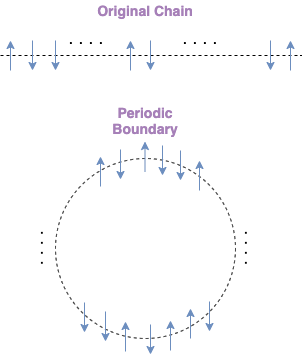
\includegraphics[width=0.4\textwidth]{Figures/Periodic_boundaries.png}
    \caption{Illustration of what a boundary condition means in the case of our spin chain.}
    \label{periodic condition}
\end{figure}
Thus, the Hamiltonian can be written in terms of the operators $\hat{d}_k$ as
\begin{equation}
H_{X Y}=\sum_{k=-(N-1) / 2}^{(N-1) / 2}\left(-\lambda+\cos \phi_{k}\right) \hat{d}_{k}^{\dagger} \hat{d}_{k}+\frac{i \gamma}{2} \sum_{k=-(N-1) / 2}^{(N-1) / 2} \sin \phi_{k}\left(\hat{d}_{k} \hat{d}_{-k}+h . c\right),
\end{equation}
where we have ignored an additional term which is proportional to $1/N$ which will vanish for in the thermodynamic limit $N\to \infty$\cite{barouch_statistical_1970,barouch_statistical_1971}, which is our case of interest.
\subsection{Bogoliubov -Valantin Transformation}
As mentioned before Fermionic quadratic Hamiltonians can be easily diagonalised via a Bogoliubov-Valantin transformation over the operators $\hat{d}_k$

\begin{equation}
\tilde{d}_{k}=u_{k} \hat{d}_{k}^{\dagger}+i v_{k} \hat{d}_{-k}.
\end{equation}
Since we want this transformation to preserve CAR, it is needed that $u_k^2 + v_k^2 = 1$, which implies that we can use the parametrization $u_{k}=\cos \left(\psi_{k} / 2\right)$ and $v_{k}=\sin \left(\psi_{k} / 2\right)$, with
\begin{equation}
\cos \frac{\psi_{k}}{2}=\frac{-\lambda+\cos \phi_{k}}{\sqrt{\left(\lambda-\cos \phi_{k}\right)^{2}+\left(\gamma \sin \phi_{k}\right)^{2}}},
\end{equation}
So finally our Hamiltonian will look as
\begin{equation}
H_{X Y}=\sum_{-(N-1) / 2}^{(N-1) / 2} \tilde{\Lambda}_{k} \tilde{d}_{k}^{\dagger} \tilde{d}_{k},
\end{equation}
with 
\begin{equation}
\tilde{\Lambda}_{k}:=\sqrt{\left(\lambda-\cos \phi_{k}\right)^{2}+\left(\gamma \sin \phi_{k}\right)^{2}},
\label{CH3:Spectrum_XY_model}
\end{equation}
where the latter expression allow us to identify the critical regions of the model.
\subsection{Fermionic Covariance Matrix for the XY model}

As we mentioned before, sometimes it turns out to be better, and useful to work directly with the Covariance matrix. To be able to do so, we need to express the Hamiltonian \eqref{CH3:Hamiltonian_XY} in terms of Majoranana fermions. This can be done by using an analogous of the Jordan Wigner transformation use to diagonalised the XY Hamiltonian but now we apply it to the $2N$ Majorana fermions

\begin{equation}
\hat{\gamma}_{l}=\left(\prod_{m<l} \hat{\sigma}_{m}^{z}\right) \hat{\sigma}_{l}^{x}, \quad \hat{\gamma}_{l+N}=\left(\prod_{m<l} \hat{\sigma}_{m}^{z}\right) \hat{\sigma}_{l}^{y},
\end{equation}
where again $l=1,2\ldots N-1$,
\begin{figure}[H]
    \centering
    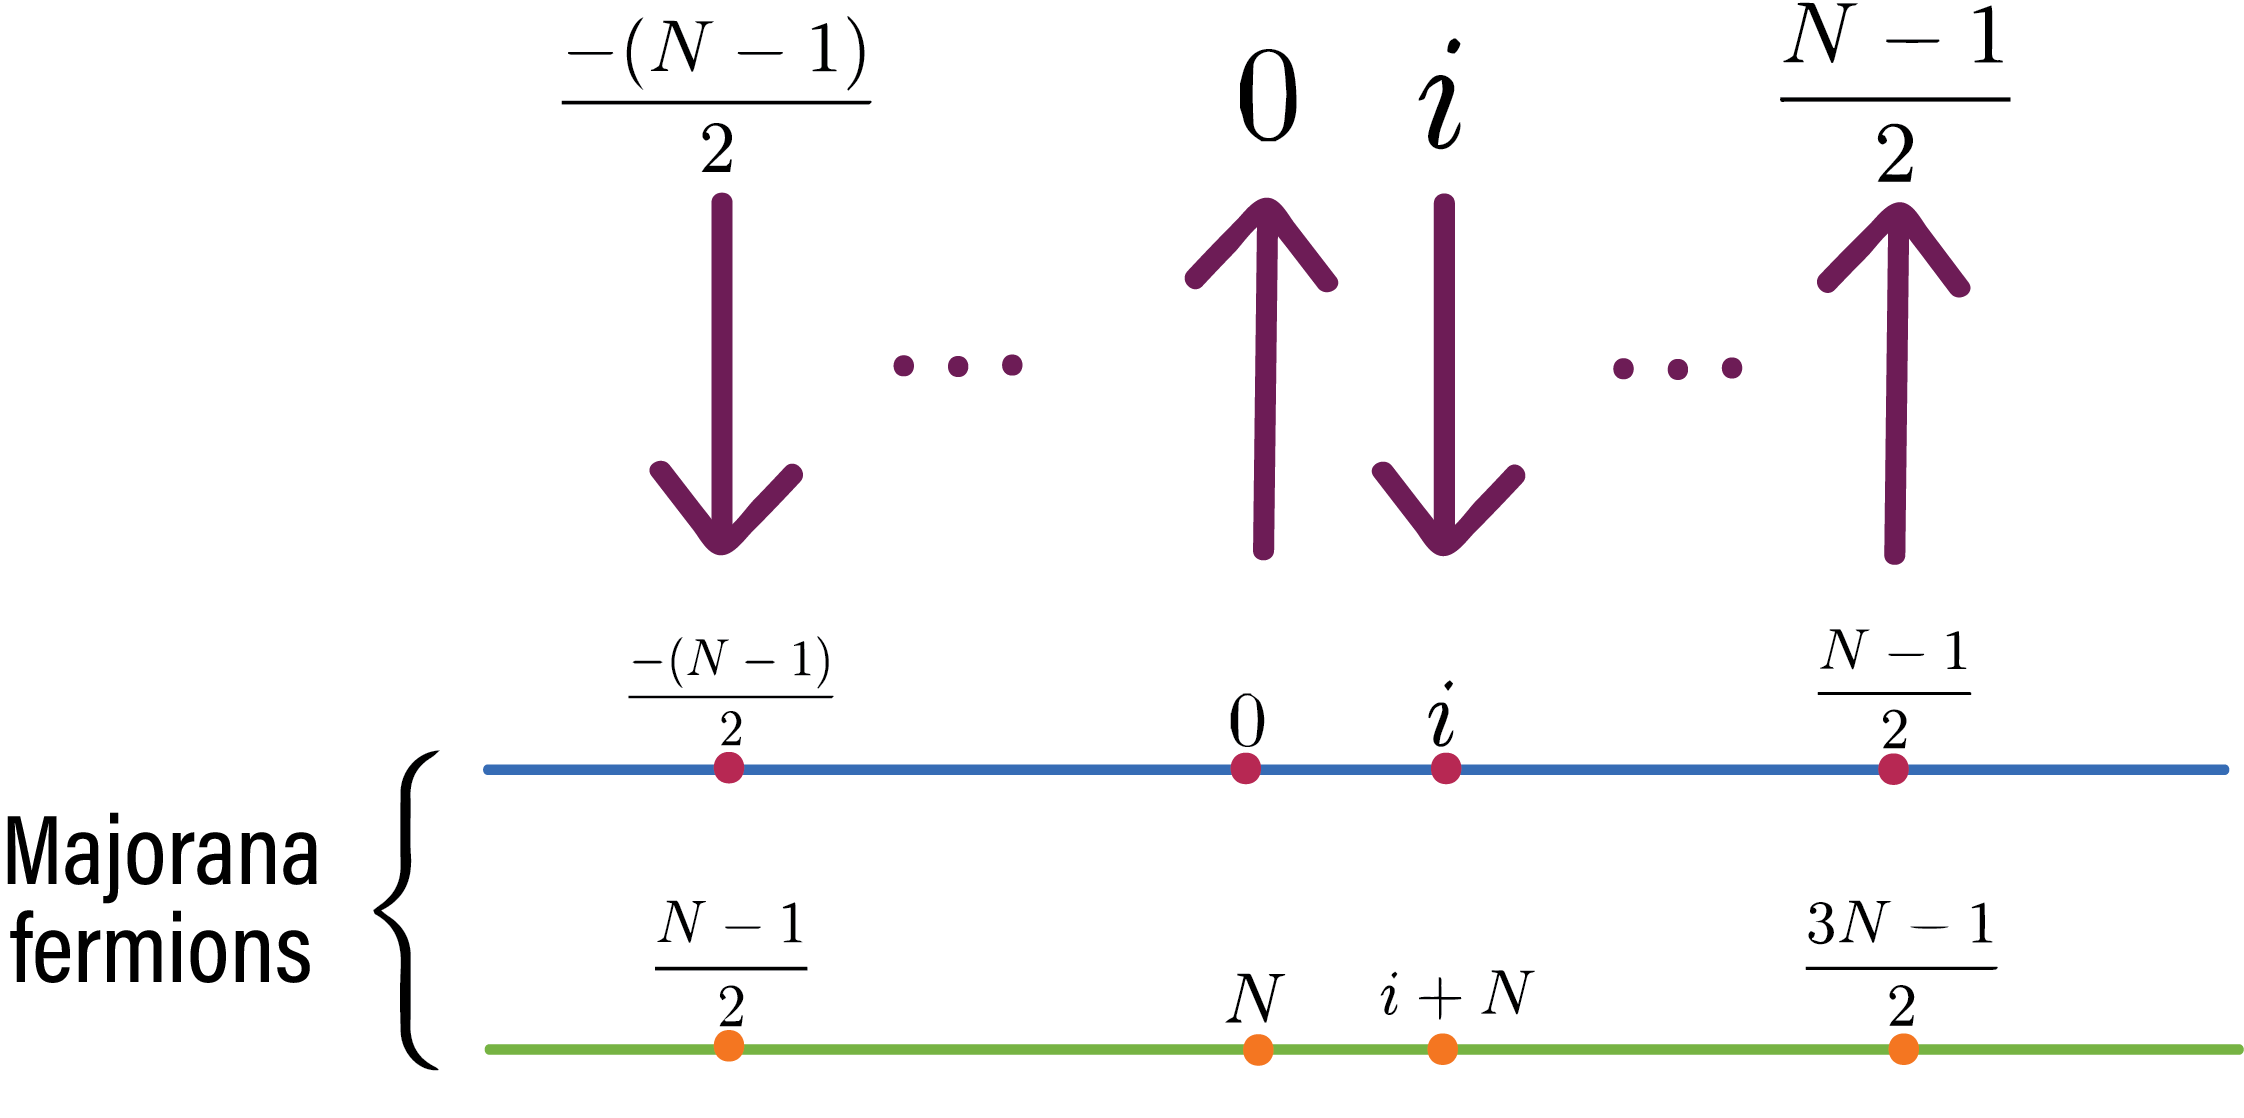
\includegraphics[width=0.5\textwidth]{Figures/ecuacion.png}
    \caption{Illustration of how the spins in the chain are mapped to the Majorana fermions.}
    \label{majorana fermions}
\end{figure}
and similarly as before we have that
\begin{equation}
\hat{\gamma}_{l} \hat{\gamma}_{l+N}=\left(\prod_{m<l} \hat{\sigma}_{m}^{z}\right)\left(\prod_{m<l} \hat{\sigma}_{m}^{z}\right) \hat{\sigma}_{l}^{x} \hat{\sigma}_{l}^{y}=i \hat{\sigma}_{l}^{z},
\end{equation}
\begin{equation}
\hat{\gamma}_{l+N} \hat{\gamma}_{l+1}=\left(\prod_{m<l} \hat{\sigma}_{m}^{z}\right) \hat{\sigma}_{l}^{y}\left(\prod_{m<l+1} \hat{\sigma}_{m}^{z}\right) \hat{\sigma}_{l+1}^{x}=\hat{\sigma}_{l}^{y} \hat{\sigma}_{l}^{z} \hat{\sigma}_{l+1}^{x}=i \hat{\sigma}_{l}^{x} \hat{\sigma}_{l+1}^{x},
\end{equation}
\begin{equation}
\hat{\gamma}_{l} \hat{\gamma}_{l+N+1}=\left(\prod_{m<l} \hat{\sigma}_{m}^{z}\right) \hat{\sigma}_{l}^{x}\left(\prod_{m<l+1} \hat{\sigma}_{m}^{z}\right) \hat{\sigma}_{l+1}^{y}=\hat{\sigma}_{l}^{x} \hat{\sigma}_{l}^{z} \hat{\sigma}_{l+1}^{y}=-i \hat{\sigma}_{l}^{y} \hat{\sigma}_{l+1}^{y}.
\end{equation}
Which coincide, up to constant factors, with the three terms in the Hamiltonian \eqref{CH3:Hamiltonian_XY}. This will lead us to a Hamiltonian of the form\cite{botero_bcs-like_2004,latorre_ground_2004}
\begin{equation}
H_{X Y}=\frac{i}{4} \sum_{\alpha, \beta=0}^{2 N} \Omega_{\alpha \beta}\left[\hat{\gamma}_{\alpha}, \hat{\gamma}_{\beta}\right],
\label{CH3:Hamiltonian_to_diagonalise}
\end{equation}
where $\Omega$ is the antisymmetric matrix of the form
\begin{equation}
\Omega=\left[\begin{array}{c|c}
0 & \tilde{\Omega} \\
\hline -\tilde{\Omega}^{T} & 0
\end{array}\right],
\label{CH3:Block_matrix}
\end{equation}
with 
\begin{equation}
\tilde{\Omega}=\begin{pmatrix}
\lambda & \frac{1-\gamma}{2} & 0 &0 &\ldots  &0 &\frac{1+\gamma}{2}\\
\frac{1+\gamma}{2} & \lambda & \frac{1-\gamma}{2} & 0 &\ldots &0 &0\\
0 & \frac{1+\gamma}{2} & \lambda & \frac{1-\gamma}{2} &\ldots &0 &0\\
\vdots& \ddots & \ddots & \ddots & \ldots &  \vdots & \vdots\\
\frac{1-\gamma}{2}&0&0&0&\ldots & \frac{1+\gamma}{2} & \lambda.
\end{pmatrix}.
\label{CH3:Hamiltonian_matrix_XY_model}
\end{equation}
In general \eqref{CH3:Block_matrix} can be diagonalised via an orthogonal transformation $O$\cite{botero_bcs-like_2004,latorre_ground_2004} \footnote{This special relation provide us a way to transform from spacial modes to excitation in the chain, so that we can either excite the chain and see what the spatial modes are or the other way.}
\begin{equation}
    \Omega=O\left[\begin{array}{c|c}
0 & \omega \\
\hline \omega & 0
\end{array}\right] O^T,
\label{CH3:Matrix_decomposed}
\end{equation}
where $O\in O(2N)$.  Writing it in terms of two smaller orthogonal matrices will look as
\begin{equation}
O=\left[\begin{array}{c|c}
O_1 & 0 \\
\hline 0 & O_2
\end{array}\right],
\end{equation}
and $\omega$ is a diagonal matrix of size $N\times N$ which holds excitation numbers $-1/2+n$. By doing the product of matrices in \eqref{CH3:Matrix_decomposed} we can easily see that 
\begin{equation}
    \tilde{\Omega}=O_1 \omega O_2^T,
\end{equation}
which is nothing but the singular value decomposition of the matrix $\tilde{\Omega}$. The latter result tell us that a fast way to construct the matrix $O$, which diagonalise $\Omega$, is to focus on $\tilde{\Omega}$.
\newline
A fact that we can exploit is that , the matrix described in equation \eqref{CH3:Hamiltonian_matrix_XY_model} $\tilde{\Omega}$ is a circulant real matrix, meaning that it can be easily diagonalised by means of a Fourier transform. So we can write
\begin{equation}
\tilde{\Omega}_{m n}=\frac{1}{N} \sum_{\theta_{k} \in(-\pi, \pi)} \omega\left(\theta_{k}\right) e^{\phi\left(\theta_{k}\right)} e^{i(m-n) \theta_{k}}.
\label{CH3:circulant_expantion}
\end{equation}
where $\omega\left(\theta_{k}\right)=\omega\left(\theta_{k}\right)^{*}=\omega\left(-\theta_{k}\right), \phi\left(\theta_{k}\right)=-\phi\left(\theta_{k}\right)$ and are given by
\begin{equation}
\omega^{2}\left(\theta_{k}\right):=\left(\lambda-\cos \theta_{k}\right)^{2}+\gamma^{2} \sin ^{2} \theta_{k},
\end{equation}
and
\begin{equation}
\phi\left(\theta_{k}\right):=\arctan \left(\frac{\lambda-\cos \theta_{k}}{-\gamma \sin \theta_{k}}\right).
\end{equation}
So expanding the equation \eqref{CH3:circulant_expantion}, we get
\begin{equation}
\begin{aligned}
\tilde{\Omega}_{m n} &=\frac{1}{N}\left[\omega(0)+(-1)^{m-n} \omega(\pi)+2 \sum_{0<\theta_{k}<\pi} \omega\left(\theta_{k}\right) \cos \left(\theta_{k}(m-n)+\phi\left(\theta_{k}\right)\right)\right] \\
&=\frac{\omega(0)}{N}+(-1)^{m-n} \frac{\omega(\pi)}{N}+\sum_{0<\theta_{k} \leq \pi} \omega\left(\theta_{k}\right)\left(u_{m}^{c}\left(\theta_{k}\right) v_{n}^{c}\left(\theta_{k}\right)+u_{m}^{s}\left(\theta_{k}\right) v_{n}^{s}\left(\theta_{k}\right)\right),
\end{aligned}
\end{equation}

where
\begin{equation}
u_{m}^{c}\left(\theta_{k}\right)=\sqrt{\frac{2}{N}} \cos \left(m \theta_{k}+\phi\left(\theta_{k}\right)\right), \quad u_{m}^{s}\left(\theta_{k}\right)=\sqrt{\frac{2}{N}} \sin \left(m \theta_{k}+\phi\left(\theta_{k}\right)\right),
\end{equation}
\begin{equation}
v_{n}^{c}\left(\theta_{k}\right)=\sqrt{\frac{2}{N}} \cos \left(n \theta_{k}\right), \quad u_{n}^{s}\left(\theta_{k}\right)=\sqrt{\frac{2}{N}} \sin \left(n \theta_{k}\right).
\end{equation}
Now defining $
u^{s}(0)=v^{s}(\pi)=0 \mathrm{y} u^{c}(0)=v^{c}(\pi)=\frac{1}{\sqrt{N}}$, we have that $\tilde{\Omega}_{m,n}$ can be written as
\begin{equation}
\tilde{\Omega}_{m n}=\sum \omega\left(\theta_{k}\right)\left(u_{m}^{c}\left(\theta_{k}\right) v_{n}^{c}\left(\theta_{k}\right)+u_{m}^{s}\left(\theta_{k}\right) v_{n}^{s}\left(\theta_{k}\right)\right).
\end{equation}
Therefore the upper part of the Hamiltonian reads
\begin{equation}
H=\sum_{m, n=0}^{N-1} \frac{i}{4} \sum_{\theta_{k}=0}^{\pi} \omega\left(\theta_{k}\right)\left(u_{m}^{c}\left(\theta_{k}\right) v_{n}^{c}\left(\theta_{k}\right)+u_{m}^{s}\left(\theta_{k}\right) v_{n}^{s}\left(\theta_{k}\right)\right)\left[\hat{\gamma}_{n}, \hat{\gamma}_{m+N}\right],
\end{equation}

\begin{equation}
H=\sum_{\theta_{k}=0}^{\pi} \omega\left(\theta_{k}\right)(\underbrace{\left[\hat{\gamma}_{k}^{c}, \hat{\gamma}_{k+N}^{c}\right]}_{1-2\sigma^{z     }_k}+\underbrace{\left[\hat{\gamma}_{k}^{s}, \hat{\gamma}_{k+N}^{s}\right]}_{1-2\sigma^{z}_k}),
\end{equation}

where
\begin{equation}
\hat{\gamma}_{k}^{c, s}:=\sum_{n} u_{n}^{c, s}\left(\theta_{k}\right) \hat{\gamma}_{n}, \quad \hat{\gamma}_{k+N}^{c, s}:=\sum_{n} v_{n}^{c, s}\left(\theta_{k}\right) \hat{\gamma}_{n+N}.
\end{equation}
Now we look back on the fact that the Fermionic covariance matrix, defined by $
\Gamma_{\alpha \beta}=\frac{1}{2 i} \operatorname{tr}\left(\rho\left[\gamma_{\alpha}, \gamma_{\beta}\right]\right)=\frac{1}{2 i}\langle \left[\gamma_{\alpha}, \gamma_{\beta}\right] \rangle$, that brings $\Omega$ into its Williamson form, does the same on the Fermionic covariance matrix. Thus for a state $|\vec{n}\rangle$, consider an eigenstate of the base $(c,s,\theta_k)$, where $m^{c, s}\left(\theta_{k}\right)-1 / 2$, with $n^{c, s}\left(\theta_{k}\right)$ the occupation number of \textit{cosine}, \textit{sine} in the $k-$mode. We get 

\begin{equation}
\begin{aligned}
\tilde{\Gamma}_{m n} &=\sum_{\theta_{k}}^{\pi}\left[m^{c}\left(\theta_{k}\right) u_{m}^{c}\left(\theta_{k}\right) v_{n}^{c}\left(\theta_{k}\right)+m^{s}\left(\theta_{k}\right) u_{m}^{s}\left(\theta_{k}\right) v_{n}^{s}\left(\theta_{k}\right)\right] \\
&=\sum_{\theta_{k}}^{\pi}\left(\frac{m^{c}\left(\theta_{k}\right)+m^{s}\left(\theta_{k}\right)}{2}\right)\left(u_{m}^{c}\left(\theta_{k}\right) v_{n}^{c}\left(\theta_{k}\right)+u_{m}^{s}\left(\theta_{k}\right) v_{n}^{s}\left(\theta_{k}\right)\right) \\
&+\sum_{\theta_{k}}^{\pi}\left(\frac{m^{c}\left(\theta_{k}\right)-m^{s}\left(\theta_{k}\right)}{2}\right)\left(u_{m}^{c}\left(\theta_{k}\right) v_{n}^{c}\left(\theta_{k}\right)-u_{m}^{s}\left(\theta_{k}\right) v_{n}^{s}\left(\theta_{k}\right)\right).
\end{aligned}
\end{equation}
by defining $m^{\pm}\left(\theta_{k}\right)=\frac{m^{c}\left(\theta_{k}\right) \pm m^{s}\left(\theta_{k}\right)}{2}$ and inverting the transformations done above, we finally get that
\begin{equation}
\tilde{\Gamma}_{m n}=\overbrace{\sum_{\theta_{k}}^{\pi} m^{+}\left(\theta_{k}\right) e^{i \phi\left(\theta_{k}\right)} e^{i(n-m) \theta_{k}}}^{\tilde{\Gamma}^{+}_{mn}}+\underbrace{\sum_{\theta_{k}}^{\pi} m^{-}\left(\theta_{k}\right) e^{i \phi\left(\theta_{k}\right)} e^{i(n+m) \theta_{k}}}_{\tilde{\Gamma}_{m n}^{-}}.
\end{equation}
We notice that $\tilde{\Gamma}^{+}_{mn}$ is circulant, whereas $\tilde{\Gamma}^{-}_{mn}$ is not, nevertheless, observe that $\tilde{\Gamma}^{+}_{mn} = \tilde{\Gamma}^{}_{mn'}$, with $n'$ a change on the index $n\to -n'$, which can be interpreted as a rotation over the circle.
\begin{figure}[H]
    \centering
    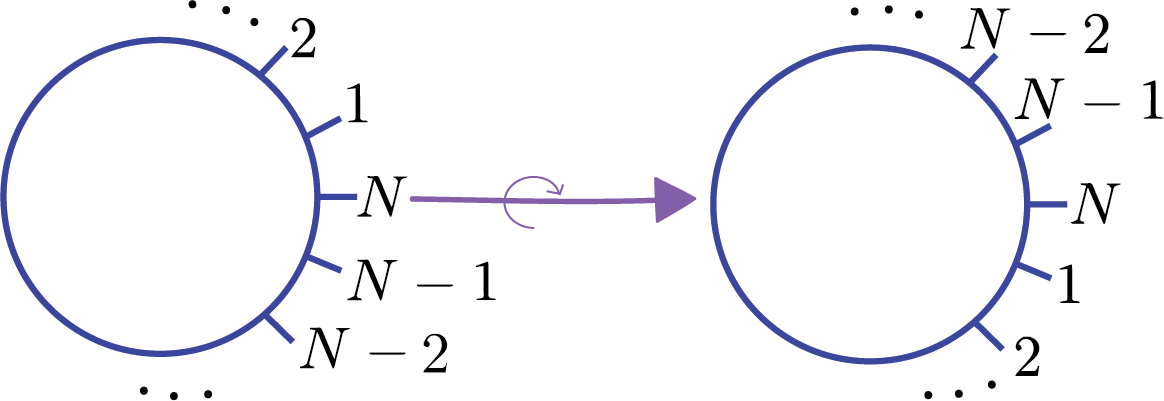
\includegraphics[width=0.6\textwidth]{Figures/Reflection_over_circle.png}
    \caption{Meaning of the relabel done in the circulant matrix, which can be seen as a reflection over the circle.}
    \label{reflectioncircle}
\end{figure}
Explicitly we can write that if $\tilde{\Gamma}^{+}_{mn}$ has the shape
\begin{equation}
\left(\begin{array}{ccccc}
a_{0} & a_{-1} & \cdots & a_{2} & a_{1} \\
a_{1} & a_{0} & \cdots & a_{3} & a_{2} \\
\cdot & \cdot & \cdot & \cdots & \cdot \\
\vdots & \vdots & \vdots & \vdots & \vdots \\
a_{-1} & a_{-2} & a_{-3} & \cdots & a_{0}
\end{array}\right),
\end{equation}
then $\tilde{\Gamma}^{-}_{mn}$ will be given by
\begin{equation}
\left(\begin{array}{ccccc}
a_{0} & a_{1} & \cdots & a_{-2} & a_{-1} \\
a_{1} & a_{2} & \cdots & a_{-1} & a_{0} \\
\cdot & \cdot & \cdot & \cdots & \cdot \\
\vdots & \vdots & \vdots & \vdots & \vdots \\
a_{-1} & a_{0} & a_{1} & \cdots & a_{-2}
\end{array}\right).
\end{equation}

So we can spot 3 things. First, the FCM always can be written as a circulant matrix plus an anticirculant matrix. Second, in the Ground state, the FCM is circulant only, since the fermion occupation numbers $n^{c}\left(\theta_{k}\right)=n^{s}\left(\theta_{k}\right)=0, \forall k$. Third, for a generic state, we have that in average the FCM matrix is always circulant, because $\langle n^{c}\left(\theta_{k}\right)\rangle=\langle n^{s}\left(\theta_{k}\right)\rangle$.\\
Now that we have showed a full characterization of the $XY$ model, we change gears and start to board our main problem. In the next section we are going to show how this is possible to find a bound in the case of the $XY$ model and even more, we will show that the mechanism for Ultra Orthogonality in this system, is indeed related with the structure of the system.


\section{Exploring ``Ultra Orthogonality''}
Now having all the tools we need we can apply what we discussed in section $2$. First we are going to look at the error exponents for the $XY$ model, we will compute the probabilities of having errors and show some numerical results. Then we move to our next problem, we will show for the $XY$ model is possible to bound the determinant and even more we find an analytical result for this determinant based on a generalisation of Szeg\"o limit theorems. 

\subsection{Error exponent}

First we recall the fact that in order to sample states at a given temperature we make use of a very well known technique, named Gibbs sampling. This technique is a special case of a Markov chain Monte Carlo algorithm. Is is well known for obtaining sequences of observations which are approximated from a specified multivariate probability distribution, It is a very useful tool for simulations in Markov processes for which the transition from which transition matrix cannot be formulated explicitly because the state space is too large\cite{robert_multi-stage_2004,gilks_markov_1996,noauthor_gibbs_nodate}. Our goal is then to sample over excited states $\ket{\vec{n}}$, where the occupations $n_q$ will be sampled independently according to the Boltzmann distribution
\begin{equation}
p(\vec{n} \mid \beta)=\prod_{q=0}^{N-1} p\left(n_{q} \mid \beta\right), \quad p\left(n_{q} \mid \beta\right)=\frac{e^{-\beta \epsilon\left(\theta_{q}\right) n_{q}}}{\sum_{n_{q}} e^{-\beta \epsilon\left(\theta_{q}\right) n_{q}}},
\label{CH3:Gibbs_Sampling}
\end{equation}
where we explicitly put the dependence of the energy with certain angle in \eqref{CH3:Gibbs_Sampling} having in mind the case of the $XY$ model\footnote{However, the $XY$ model is not the only model in which the energy can be parametrized in terms of an angle, in general it has been shown that every one-dimentional translationally invariant closed chain of free Fermions/Bosons will have this property \cite{eisert_area_2010,fradkin_field_1997,katsura_statistical_1962,latorre_ground_2004,lieb_two_1961}.}. The goal of using this technique  that the size of the Hilbert space is to find the probability distribution with a given temperature $\beta$. It is well known that in the Fermionic case, the average number of excitations in the mode at angle $\theta$ is given by
\begin{equation}
f\left(\theta_{q} \mid \beta\right) \equiv\left\langle n_{q}\right\rangle_{\beta}=\frac{1}{e^{\beta \epsilon\left(\theta_{q}\right)} + 1},
\end{equation}
while the variance in the number of excitations is given by

\begin{equation}
v\left(\theta_{q} \mid \beta\right) \equiv\left\langle n_{q}^{2}\right\rangle_{\beta}-\left\langle n_{q}\right\rangle_{\beta}^{2}=\frac{1}{e^{\beta \epsilon\left(\theta_{q}\right)} + 1}=f\left(\theta_{q}\right)\left(1 - f\left(\theta_{q}\right)\right).
\end{equation}
With this method of sampling, the mean energy is 
\begin{equation}
\langle E\rangle_{\beta}=\sum_{q} f_{q}\left(\theta_{q} \mid \beta\right) \epsilon_{q}\left(\theta_{q}\right)=N \oint_{N} \frac{d \theta}{2 \pi} f(\theta \mid \beta) \epsilon(\theta),
\end{equation}
where $\oint$ denote the Riemann sum approximation to the respective integral with $N$ subdivisions. As we mentioned before we are interested in the limit $N\to\infty$, we will replace the sums by its correspondent integral. Similarly we can compute the energy variance of the sampled states 
\begin{equation}
\left\langle\Delta E^{2}\right\rangle_{\beta}=\sum_{q} v_{q}\left(\theta_{q} \mid \beta\right) \epsilon_{q}^{2}\left(\theta_{q}\right)=N \oint_{N} \frac{d \theta}{2 \pi} v(\theta \mid \beta) \epsilon^{2}(\theta).
\end{equation}
Thus Gibbs sampling provides an even sampling of states within $\Delta E$ of the energy $\langle E\rangle$, where $\Delta E/\langle E\rangle\sim O(N^{-1/2})$.\\
Thinking back on the case of the $XY$ model, the ensemble defined by Gibbs sampling is nothing but the canonical ensemble defined on the full chain, with thermal density matrix
\begin{equation}
\rho_{T}(\beta, N)=\sum_{\vec{n}} p(\vec{n} \mid \beta)|\vec{n}\rangle\langle\vec{n}|=\frac{e^{-\beta H_{N}}}{Z(\beta, N)}, \quad \log Z(\beta, N)= N  \oint_{N} \frac{d \theta}{2 \pi}\log \left(1 \pm e^{-\beta \epsilon(\theta)}\right).
\end{equation}
This thermal state defines a reduced density matrix in the subchain of length $L$
\begin{equation}
\left.\rho(\beta, N)\right|_{L} \equiv \operatorname{Tr}_{N-L} \rho_{T}(\beta, N),
\end{equation}
which is expected to correspond to the local thermal state,
\begin{equation}
 \left.\rho(\beta, N)\right|_{L} \simeq \rho_{T}(\beta, L) \equiv \frac{e^{-\beta H_{L}}}{Z(\beta, L)},
\end{equation}
 for $L$ sufficiently larger in comparison to the correlation length, in which the boundary effects can be neglected. Since we know this states conserve Gaussianity under partial traces, the reduced state $\left.\rho(\beta, N)\right|_{L}$ will be also Gaussian, meaning that the state will be uniquely characterised by its covariance matrix. This arguments lead us to the conclusion that the Gibbs average of the reduced partial density matrices $\rho_L(\vec{n})$ satisfies
 \begin{equation}
 \left.\rho(\beta, N)\right|_{L}=\left\langle\rho_{L}(\vec{n})\right\rangle_{\beta}.
 \end{equation}
The latter series of arguments where need to understand why this method of sampling is appropriate for our purpose. Even more, it provide us an expression to the probability of having and excitation (a $1$) or not ($0$). Having said that, we move gears to the computing the probability of having an error over two independent sequences. We can write this probability in terms of our energy as and a given $\theta_k$
\begin{equation}
n(\theta_k)=\frac{1}{1+e^{\beta(\Omega(\theta_k)-\Omega^*)}},
\end{equation}
where $\Omega(\theta_k)$ is given by equation \eqref{CH3:Spectrum_XY_model}, and $\Omega^*$ correspond to the minimum of energy\footnote{It is not hard to check that the minimum of energy happens at $\theta^*=\pm \operatorname{acos}\left(-\frac{\lambda}{1-\gamma^2}\right)$ with value
\[\sqrt{\frac{\gamma^2(\gamma^2-1+\lambda^2)}{(\gamma^2-1)}}\]}. Then the probability of two sequences not having an error in the position $k$ will be given by
\begin{equation}
1-p(\theta_k) = n(\theta_k)^2 + (1-n(\theta_k))^2 = \frac{1}{1+\operatorname{sech}\left(\beta(\Omega(\theta_k)-\Omega^*)\right)},
\end{equation}
and then the probability of having an error will be given by
\begin{equation}
p(\theta_k) = n(\theta_k)^2 + (1-n(\theta_k))^2 = \frac{1}{1+\cosh\left(\beta(\Omega(\theta_k)-\Omega^*)\right)},
\end{equation}
So the expected value of the number of errors $X=\sum_{k}X(\theta_k)$ is given by

\begin{equation}
\mu = \sum p(\theta_k) \stackrel{N\to \infty}{=}\frac{N}{2\pi}\oint d\theta \frac{1}{1+\cosh{(\beta(\Omega(\theta)-\Omega^*)})}.
   \label{CH3:average_of_errors}
\end{equation}
In Figure \ref{CH3:examples_of_probability_distribution_errors}, we showthe behaviour of the probability distribution as a function of the angle. 
\begin{figure}[H]
\centering
\begin{subfigure}[b]{0.47\textwidth}
    \centering
    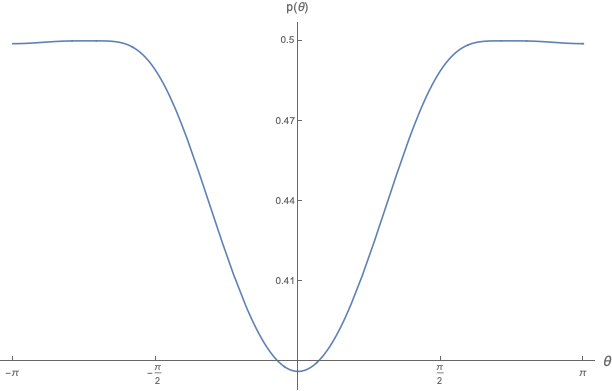
\includegraphics[width = \textwidth]{Figures/beta_1.png}
    \caption{Probability distributions of errors as a function of the position in the chain. this plot correspond to a value of $\beta=1$.}
    \label{beta1}
\end{subfigure}
\hfill
\begin{subfigure}[b]{0.47\textwidth}
    \centering
    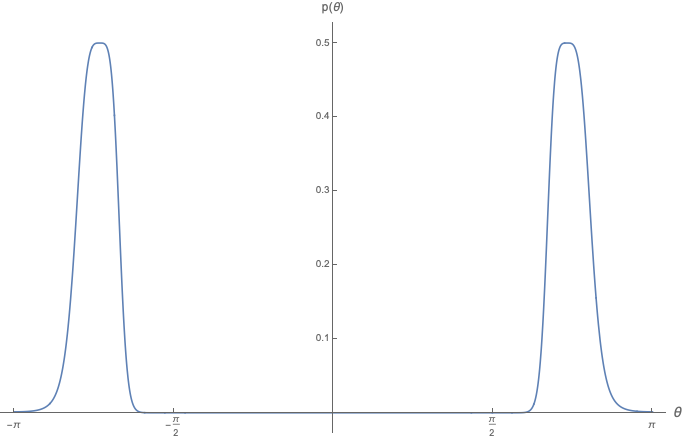
\includegraphics[width = \textwidth]{Figures/beta_80.png}
    \caption{Probability distributions of errors as a function of the position in the chain. this plot correspond to a value of $\beta=80$.}
    \label{beta80}
\end{subfigure}
\caption{An illustration of how the function $p(\theta_k)$ behaves as a function of the angle $\theta$. As we can see in both figures there are regions of the chain in which the probability of having an error is smaller.}
       \label{CH3:examples_of_probability_distribution_errors}
\end{figure}


\chapter{Conclusions and Perspectives}

Throughout all this document, we have exposed a series of arguments to show, the way Ultra Orthogonality could be an alternative mechanism for understanding equilibration.  As we mentioned, this is connected to thermalisation problem, since for most systems thermal typicality is expected, thus the state of equilibrium we end with has to be nothing but the canonical state. Additionally, we tackle the problem when Ultra Orthogonality holds exactly, that means, the equilibrium state is automatically reached by computing the correspondent reduced state of the Universe. By this, we mean that we have led all our efforts to show that for the case of Fermionic systems, there exists a particular sort of pure dynamical states, such that when taking its correspondent partial trace over the environment, these resultant reduced states are automatically in its correspondent equilibrium, and the way to understand this phenomena, can be through an information theory viewpoint, whereby, the fact that we work over a finite algebra, as the one in fermions, let us formulate this particular problem in terms of minimum distance codes.\\



\indent Not satisfied with finding this result in a virtual general way for Fermionic systems, we decided to estimate the size of the correspondent Hilbert subspace associated with the states that fulfil Ultra Orthogonality, in the sense that all reduced states, will be automatically stationary states (Constant states over time). Thanks the formalism of exponent errors, used in Code Theory , it was possible to provide an expression to the large deviation present in the Fermionic systems, namely, this exponent tell us the an estimate about the expected number of random Fermionic minimum codes that fulfil Ultra Orthogonality, Which as we show, whenever this exponent is larger than zero, we therefore are able to show that the correspondent Hilbert subspace to these states is exponentially large. In other words, aside of our result being quite general, we found that whenever the correspondent exponent, which depends on the parameters of the system, is larger than zero, we will have a huge Hilbert subspace (exponentially large), which contains states such that when taking the partial trace over its correspondent environment are automatically equilibrated.\\

\indent This particular result bring more questions than answers. One of the first questions we may ask is, what happens if instead of thinking this problem only in terms of random codes, we impose a condition over the energy?. From our point of view, we consider that this could be the main key to connect all this results with the thermalisation problem, indeed we think that even though, the the exponent error must change, we could still find situations in which it is grater than zero, and therefore, find that the expected number of codes at certain energy will also follow a large deviation law. The problem we stumble upon was that when imposing a restriction over the energy for the codewords, liner superposition may end up not conserving the restriction of energy, so another study will be needed to confirm if this can be done and provide the connection to thermalisation.

\indent Finally, we want to point out that the physical meaning of these quantities was not discussed, and maybe the question of  what exactly is the physical meaning of these exponents? could have emerge at some point without any answer. What we wanted to stress here is that indeed, there was an attempt to find some physical interpretation about these quantities. Specifically, we tried to tackled this matter by studying the one dimensional $XY$ model of spins $1/2$. The choice for this particular system, was due to the fact that this particular system can be analytically solved with efficient algorithms. In spite of our efforts, hitherto, a complete interpretation or an intuition of our result have not been found. Thus we emphasise this point as a future work to be done in this subject.





%\include{Kap4/Kap4}
%\include{Kap5/Kap5}
%\begin{appendix}
\chapter{Dynamics of density matrix.}\label{AppendixA}
\section{Schr{\"o}dinger equation.}
A particular fact about the Schr{\"o}dinger equation is that it can not be derived from any mathematical formalism, its construction is phenomenological and can be seen as a postulate of quantum mechanics.\\
The Schr{\"o}dinger equation is written as follows:
\begin{equation}
i\hbar\frac{d}{dt}\ket{\psi(t)}=\hat{H}\ket{\psi(t)} \ ;\qquad \hat{H}=\hat{H}^{\dagger}
\label{scrodingereq}
\end{equation}
Some facts about this equation are:
\begin{itemize}
\item Is linear and first order in time.
\item It is deterministic.
\item Given $\ket{\psi(t)}$ and $\hat{H}$ it fixes $\ket{\psi(t')}$ for all $-\infty <t'<\infty$
\item As the operator $\hat{H}$ is hermitian Schr{\"o}dinger the equation for $\bra{\psi(t)}$ is simply given by:
\[-i\hbar\bra{\psi(t)}=\bra{\psi}\hat{H}\]

\item It preserves the norm of $\ket{\psi(t)}$.
\vspace{.5mm}
\begin{align*}
\bra{\psi}\ket {d\psi}+\bra{ d\psi}&\ket{ \psi}=\bra{\psi}\frac{-i}{\hbar}dt \hat{H}\ket{\psi}+\bra{\hat{H}\psi}\frac{i}{\hbar}dt\ket{\psi}\\
&=\frac{-i}{\hbar}dt\left(\bra{\psi}\hat{H}\ket{\psi}-\bra{\psi}\hat{H}\ket{\psi}\right)=0
\end{align*}

\[\frac{d}{dt}\mid\psi\mid^2=\frac{d}{dt}\bra{\psi}\ket{\psi}=0 \ ; \quad\mid\psi\mid=constant\]

\end{itemize}
With these properties we can then construct the evolution of the density matrix $\rho=\ket{\psi}\bra{\psi}$, by considering the evolution of $\rho$ given by the Schr{\"o}dinger equation:
\begin{equation}
i\hbar\frac{d}{dt}\ket{\psi}\bra{\psi}=\hat{H}\ket{\psi}\bra{\psi}-\ket{\psi}\bra{\psi}\hat{H}=\left[\hat{H},\rho\right],
\label{liouville-vonnuemann}
\end{equation}
this equation is also called Liouville-von Neumann equation in the Schr{\"o}dinger picture.\\
Following the same formalism, in the Heisenberg picture we see that the evolution of an operator $\hat{A}$ is given by:
\[i\hbar\frac{d}{dt}\hat{A}_H=\left[\hat{A}_H,\hat{H}_H\right]\]
Where $\hat{A}_H=\hat{U}^{\dagger}\hat{A}\hat{U}$ with $\hat{U}$ an unitary transformation. And the average of an operator $\hat{A}$ with respect to an  of states is given by:

\begin{align}
\sum_{n}p_n\bra{\psi_n}\hat{A}\ket{\psi_n}&=\sum_n p_n \text{tr}[\bra{\psi_n}\hat{A}\ket{\psi_n}] \nonumber \\
&=\sum_n p_n\text{tr}[\hat{A}\ket{\psi_n}\bra{\psi_n}] \nonumber \\
&=\text{tr}\left[\hat{A}\sum_n p_n\ket{\psi_n}\bra{\psi_n}\right]\nonumber\\
&=\text{tr}(\hat{A}\rho) \nonumber \\
&=\braket{\hat{A}} 
\label{appendixexpectedvalue}
\end{align} 

%%%%-------- Decoherence Part----------%%%%%
\section{Decoherence.}\label{appendixAdecoherence}
From the Schr{\"o}dinger equation one knows that a way to talk about quantum dynamics is in terms of unitary transformations. If a system undergoes Hamiltonian evolution for a finite time then the evolution can be described by an unitary operator $U$. In this case $\ket{\psi}\bra{\psi}$ is mapped to $U\ket{\psi}\bra{\psi}U^{\dagger}$, and by linearity, a general density matrix $\rho$ is then mapped to $U\rho U^{\dagger}$.\\
In such wise, unitary operators correspond to reversible operations or in other words, if $U$ is valid unitary time evolution then so is $U^{\dagger}$. In terms of Hamiltonians, evolution according to $-H$ will reverse evolution according to $H$. But other quantum processes such as non unitary evolution cause an irreversible loss of information.\\
To illustrate it, let's first start understanding the concept of \textit{mixture}.Mixture refers to \\

If a state $\ket{\psi_{a}}$ has a probability $p_a$ to happen, then the density matrix is $\sum_{a}p_{a}\ket{\psi_{a}}\bra{\psi_{a}}$. But in the case we've got an ensemble of density matrices $\{(p_1,\rho_1),\ldots,(p_m,\rho_m)\}$.Then the ``average'' density matrix is\footnote{This is also called a time-independent mixture.}
\begin{equation}
\rho=\sum^{m}_{a=1}p_a\rho_a.
\label{rhoapendixA}
\end{equation}
With this in mind we can use it to model \textit{random unitary evolution}, by supposing our state experiences a random Hamiltonian. Thus the correspond mapping it results by considering that unitary $U_{a}$ occurs with probability $p_a$ for $a=1,\ldots,m$, is:
\begin{equation}
\rho\longrightarrow \sum_{a=1}^{m}p_a U_a \rho U_{a}^{\dagger}.
\label{Mapping}
\end{equation}
To understand how under this mapping we can explain the loss of coherence in simple quantum systems let's check two examples.
\subsection{Evolution of polarised light.}
Suppose we start with a density matrix
\[
\rho=
  \left( 
  {\begin{array}{cc}
   \rho_{11} & \rho_{12} \\
   \rho_{21} & \rho_{22} \\
  \end{array} }
   \right),
\]
and choose a random unitary evolution which is going to perform as follows: With probability $1-p$ the matrix $\rho$ remains invariant and with probability $p$ we perform a unitary transformation corresponding to $\hat{\sigma}_z$%\footnote{This is the case of the evolution of polarized light which is observed in the $\hat{z}$ basis.}. 
then the ensemble of unitary transformations we are working with is given by $\{(1-p,I),(p,\hat{\sigma}_z)\}$. So the density matrix is mapped to:
\begin{align*}
\rho ' &\equiv (1-p)\hat{\mathds{1}}\rho \hat{\mathds{1}}^{\dagger} + p\hat{\sigma}_z \rho \hat{\sigma}_z^{\dagger}\\[0.5cm]
&=\left(
{\begin{array}{cc}
\rho_{11} & (1-2p)\rho_{12} \\
(1-2p)\rho_{21} & \rho_{22} \\
\end{array}
}
\right).
\end{align*}
First we can see two trivial different cases:
\begin{enumerate}
\item If $p=0$, of course nothing happen and the matrix remains invariant.
\item If $p=1$, we simply get $\rho$ changes as: $\rho'=\hat{\sigma}_z \rho \hat{\sigma}_z^{\dagger}$, which is translate as an unitary transformation of the density matrix.
\end{enumerate}
One can observe that the diagonal terms remain invariant, whereas the terms off-diagonal are reduced in absolute value in consequence of $\mid1-2p\mid<1$. Thus, we see the diagonal terms correspond to the probability of outcomes we would observe being in the $\hat{z}$ basis, so, it's clear that a rotation along $\hat{z}$ would not affect the results. However, the off-diagonal terms will vanish when $p=1/2$, meaning that the polarization in $\hat{x}$ and $\hat{y}$ directions has been eliminated. A way to explain why this is happening we use the fact that  the density matrix state for a two-level system can be written using the Pauli operators as:
\begin{equation}
\rho=\frac{1}{2}\left[\hat{\mathds{1}}+x\hat{\sigma}_x+y\hat{\sigma}_y+z\hat{\sigma}_z\right].
\label{Blochapendix}
\end{equation}
Where $x,y,z$ are the averages of the Pauli operators, this is $x=\textnormal{Tr}[\hat{\sigma}_x\rho]$ etcetera.Then by using the relation between the product of these operators:
\[
\hat{\sigma}_i\hat{\sigma}_j=\delta_{ij}\hat{\mathds{1}}+i\epsilon_{ijk}\hat{\sigma}_k.
\]
We can prove that:
\[
\hat{\sigma}_z\rho\hat{\sigma}_z^{\dagger}=\rho=\frac{1}{2}\left[\hat{\mathds{1}}-x\hat{\sigma}_x-y\hat{\sigma}_y+z\hat{\sigma}_z\right].
\]
Finally for the case of $p=1/2$ we see that:
\begin{equation}
\rho'=\frac{1}{2}(\rho+\hat{\sigma}_z\rho\hat{\sigma}_z^{\dagger})= \frac{1}{2}\left[\hat{\mathds{1}}+z\hat{\sigma}_z\right].
\label{rhoprime}
\end{equation}
As we see in equation \eqref{rhoprime} the possible values over $x$ and $y$ have been removed,this means, the polarization in the  $\hat{x}-\hat{y}$ plane has been eliminated.\\
So with this example we illustrated that:
\begin{itemize}
\item Decoherence destroys some quantum/wave-like effects, such as interference.
\item Decoherence also involves the loss of information, which in  this case was the phase information.

\end{itemize}
\subsection{Spontaneous emission.}\label{spontaneous emission}
Let's consider an atom with states $\ket{g}$ and $\ket{e}$, that correspond to ``ground'' and ``excited'' state. Suppose the initial state of the system is given by 
$\ket{\psi}_{\text{atom}}\otimes \ket{0}_{\text{photon}}$ with $\ket{\psi}=c_1\ket{g}+c_2\ket{e}$.
 Then these will interact via the Jaynes-Cumming Hamiltonian.
\[{\hat  {H}}_{{{\text{JC}}}}=\hbar \omega _{c}{\hat  {a}}^{{\dagger }}{\hat  {a}}+\hbar \omega _{a}{\frac  {{\hat  {\sigma }}_{z}}{2}}+\frac  {\hbar \Omega }{2}\left({\hat  {\sigma }}_{+}\otimes{\hat  {a}}+{\hat  {\sigma }}_{-}\otimes{\hat  {a}}^{{\dagger }}\right).\]
That for simplicity we ignore the fist terms resulting the next Hamiltonian:

\begin{equation}
H=\frac  {\hbar \Omega }{2}\left({\hat  {\sigma }}_{+}\otimes{\hat  {a}}+{\hat  {\sigma }}_{-}\otimes{\hat  {a}}^{{\dagger }}\right).
\label{hamiltonianjaynes-cummings}
\end{equation}
If the atom and photon interact via this Hamiltonian for a time $t$. Replacing $\delta\equiv\Omega t/2$, an expansion in powers of $\delta$, for $\mid\delta\mid<<1$ is:

\[e^{-\frac{i\hat{H}t}{\hbar}}\ket{\psi}\otimes\ket{0}=(c_1\ket{g}+c_2\ket{e})\otimes\ket{0}-i\delta c_2\ket{g}\otimes\ket{1}-\frac{\delta^2}{2}c_2\ket{e}\otimes\ket{0}+O(\delta^3).\]

We measure and we see that with probability $\mid c^2_2\mid\delta^2$ the photon number is 1 and the state of the atom is a ground state $\ket{g}$. We could be tempted to conclude that before the measurement the state of the system was the excited state, nonetheless, contrary to what we think, the only thing we can conclude from this result is that $c_2$ must is non-zero. And the reason why we say this is because with probability\footnote{To compute this probabilities for the state $i$ on the photon we calculate:
\[\bra{\psi}\otimes\bra{0}e^{\frac{i\hat{H}t}{\hbar}}\left[\hat{\mathds{1}}\otimes\ket{i}\bra{i}\right]e^{-\frac{i\hat{H}t}{\hbar}}\ket{\psi}\ket{0}.\]
And we keep until terms of order $\delta^2$}
 $\mid c_1\mid^2+(1-\delta^2)\mid c_2 \mid^2=1-\mid c_2 \mid^2\delta^2$  we observe 0 photons and the state is different than the ground state as we could thought. Instead, the state is a linear combination of the ground and excited state.
\[\frac{c_1\ket{g}+(1-\delta^2)c_2\ket{e}}{\sqrt{1-\mid c_2\mid^2\delta^2}}.\]
Of course this is the result considering only terms up to $O(\delta^3)$, now if we wait long enough we must consider more terms in the expansion and this will leads us to a probability of 0 or 1 in the case of having photon number 1 and 0 respectively. This result turns out to be classic and in consequence it means that if we wait enough time, quantum systems subject to an external interaction will loose their quantum coherence.

\begin{figure}[h!]
\centering
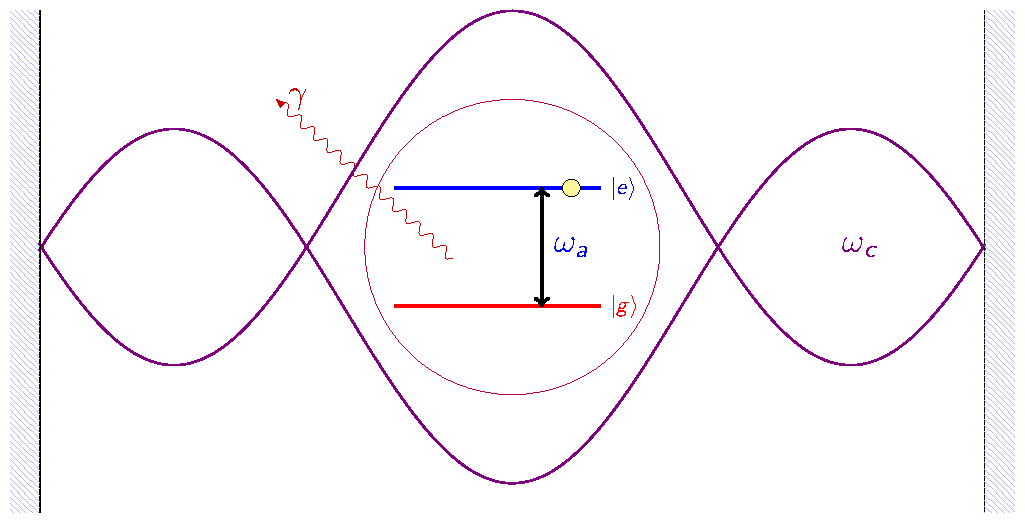
\includegraphics[width=0.7\textwidth]{Figures/presentationI.pdf}
\caption{Sketch of the situation considered by the Hamiltonian of Jaynes-Cummings.}
\label{Jaynescummings}
\end{figure}

%%%%-------- Partial measurements----------%%%%%
\section{Partial measurement and partial trace.}\label{appendixAparcialtrace}



Density matrices were introduced by the purpose of understand how is encode all the accessible information about a quantum mechanical system. It turns out that the ``pure'' states described by vectors $\ket{\psi}$ on Hilbert space\footnote{It is always possible to find a vector representation for a given quantum system. This can be done via the Gelfand-Neumark-Segal construction.}, are idealised descriptions that cannot characterize statistical mixtures which often occur in nature.  
Let's consider two systems $A$, $B$, with associate Hilbert spaces $\mathcal{H}_A$ and $\mathcal{H}_B$ respectively. If the state of the joint system $AB$ with Hilbert space $\mathcal{H}=\mathcal{H}_A\otimes\mathcal{H}_B$ is pure then it is possible that the states of $A$ and $B$ are not themselves pure. However, if there is a density matrix $\rho_{AB}$ that describes the joint state of these systems then we should be able to define density matrices for the individual systems.In fact for any observable $X:\mathcal{H}\rightarrow\mathcal{H}_{i}$, with $\mathcal{H}_{i}\subset\mathcal{H}$, $A$ or $B$ should have well-defined expectation value, and this can be used to define a reduced matrix for the system $A$ or $B$. Mathematically we denote the density matrix of system $A$ by $\rho_A$, and this matrix has to satisfy:
\begin{equation}
\text{tr}[\rho_AX]=\text{tr}[\rho_{AB}(X\otimes\mathds{1}).]
\label{partialdensitymatrix}
\end{equation}
One can proof that this density matrix is unique and always exist. similarly we can define the state of the system $B$ to be $\rho_B$ by satisfying $\text{tr}[\rho_BX]=\text{tr}[\rho_{AB}(\mathds{1}\otimes X)]$.\\
Writing explicitly  \eqref{partialdensitymatrix}:
\[
\sum_{a,a'}\rho_{A,a,a'}X_{a,a'}=\sum_{a,b,a',b'}
\rho_{AB,ab,a'b'}X_{a,a'}\delta_{b,b'}=\sum_{a,a',b}
\rho_{AB,ab,a'b}X_{a,a'}.
\]
Since this should be valid for any observable $X$ we get:
\[\rho_{A}=(\text{tr}_B[\rho])_{a,a'}=\sum_b\rho_{AB,ab,a'b}.\]

So from this result it seems like if we take the trace over $B$ while leaving $A$ alone we can compute the expression in  \eqref{partialdensitymatrix}. From the latter result we can see that the \textit{partial trace} is a map $\mathcal{L}$ such that: $\mathcal{L}_{B}(\mathcal{H})\rightarrow\mathcal{H}_{A}$ for the case of taking the trace over $B$, and we can compute the density matrix as: $\rho_{A}=\text{tr}_{B}[\rho_{AB}]$. The partial trace is the quantum analogue of the rule for marginals of probability distributions: $p_{X}(x)=\sum_{y}p_{XY}(x,y)$.\\
A similar equation holds for 
$\rho_B\equiv\text{tr}_B[\rho_{AB}]$
 which can be expressed in terms of matrix elements as
\[
\rho_{B,b,b'}=(\text{tr}[\rho])_{b,b'}=\sum_a\rho_{AB,ab,ab'}.
\]

To illustrate in a better way the way we can compute this partial trace, let's see the example of spontaneous emission from \ref{spontaneous emission}.
\[
\ket{\psi}=e{\frac{i}{\hbar}\hat{H}t}\frac{\ket{g}+\ket{e}}{\sqrt{2}}\otimes\ket{0}.
\]
With $\hat{H}=\Omega(\ket{g}\bra{e}\otimes\hat{a}^{\dagger}+\ket{e}\bra{g}\otimes\hat{a}$. $\hat{H}\ket{g,0}=0$ and $\hat{H}$ acts on the $\{\ket{e,0},\ket{g,1}\}$ subspace as a rotation. Thus:
\[
\rho=\ket{\psi}\bra{\psi}=\bordermatrix{~&\bra{g,0}&\bra{e,0}&\bra{g,1}&\bra{e,1}\cr
			\ket{g,0}&\frac{1}{2} & \frac{1}{2}\cos\theta & \frac{i}{2}\sin\theta & 0\cr
			\ket{e,0}&\frac{1}{2}\cos\theta & \frac{1}{2}\cos^2\theta & \frac{i}{2}\cos\theta\sin\theta & 0\cr
			\ket{g,1}&-\frac{i}{2}\sin\theta & -\frac{i}{2}\sin\theta\cos\theta & \frac{1}{2}\sin^2\theta & 0\cr
			\ket{e,1}&0 & 0 & 0 & 0\cr}
\]
The reduced state of the atom is
\[
\text{tr}_{photon}\ket{\psi}\bra{\psi}=
\bordermatrix{~&\bra{g}&\bra{e}\cr
			\ket{g}&\frac{1}{2}+\frac{1}{2}\sin^2\theta & \frac{1}{2}\cos\theta\cr
			\ket{e}&\frac{1}{2}\cos\theta & \frac{1}{2}\cos^2\theta\cr},
\]

and the reduced state of the photon is:

\[
\text{tr}_{atom}\ket{\psi}\bra{\psi}=\bordermatrix{~&\bra{0}&\bra{1}\cr
			\ket{0}&\frac{1}{2}+\frac{1}{2}\cos^2\theta & \frac{i}{2}\sin\theta\cr
			\ket{1}&-\frac{i}{2}\sin\theta & \frac{1}{2}\sin^2\theta\cr}.
\]
%%%%-------- Interaction picture----------%%%%%
\chapter{The Interaction Picture.}\label{appendixBinteractionpicture}

Sometimes express the operators and states in other equivalent representation or ``picture'' is of great importance in solving problems in quantum mechanics in a perturbative fashion.
We begin by considering a Hamiltonian of the form:
\begin{equation}
\hat{H}=\hat{H}_0 +\hat{V}.
\label{eq1interaction}
\end{equation}
Here $\hat{H}_0$ denotes the part of the Hamiltonian that describes the free or unperturbed evolution of the system $\mathcal{S}$, whereas $\hat{V}$ is some added external perturbation. From standard quantum theory, we know that the expectation value of an operator observable $\hat{A}(t)$ is given by the trace as in \eqref{appendixexpectedvalue}.
\begin{equation}
\braket{\hat{A}(t)}=\text{tr}\left[\hat{A}(t)\rho(t)\right]=\text{tr}\left[\hat{A}(t)e^{-\frac{i}{\hbar}\hat{H}t}\rho(0)e^{\frac{i}{\hbar}\hat{H}t}\right].
\label{eq2interactionpicture}
\end{equation}
But by using the fact that the trace is invariant under cyclic permutations of the arguments ($\text{tr}(\hat{A}\hat{B}\hat{C}\ldots)=\text{tr}(\hat{B}\hat{C}\ldots\hat{A})$) the expected value of $\hat{A}$ can be written as:
\begin{equation}
\braket{\hat{A}(t)}=\text{tr}\left[\left(e^{\frac{i}{\hbar}\hat{H}_0 t}\hat{A}(t)e^{-\frac{i}{\hbar}\hat{H}_0 t}\right)\left(e^{\frac{i}{\hbar}\hat{H}_0 t}e^{-\frac{i}{\hbar}\hat{H}t}\rho(0)e^{\frac{i}{\hbar}\hat{H}t}e^{-\frac{i}{\hbar}\hat{H}_0t}\right)\right].
\label{eq3interactionpicture}
\end{equation}
Equation  \eqref{eq3interactionpicture} take us to now introduce the \textit{interaction-picture}form of general operators $\hat{A}(t)$ and density matrices $\rho(t)$ as:
\begin{equation}
\hat{A}_I(t)=e^{\frac{i}{\hbar}\hat{H}_0t}\hat{A}(t)e^{-\frac{i}{\hbar}\hat{H}_0t},
\label{eq4interactionpicture}
\end{equation}
\begin{align}
\label{eq5interactionpicture}
\begin{split}
\rho_I(t)&=e^{\frac{i}{\hbar}\hat{H}_0t}\rho(t)e^{-\frac{i}{\hbar}\hat{H}_0t}
\\
&=e^{\frac{i}{\hbar}\hat{H}_0t}e^{-\frac{i}{\hbar}\hat{H}t}\rho(0)e^{\frac{i}{\hbar}\hat{H}t}e^{-\frac{i}{\hbar}\hat{H}_0t}.
\end{split}
\end{align}
Here the subscript $I$ is used to refer interaction-picture operator. As we note, the dynamics in the interaction-picture is determined by the  Hamiltonian ($\hat{H}_0$) instead of the total Hamiltonian ($\hat{H}$). Hence with equations \eqref{eq4interactionpicture} and \eqref{eq5interactionpicture} the expected value can be written as:
\begin{equation}
\braket{\hat{A}(t)}=\text{tr}(\hat{A}_I(t)\rho_I(t)).
\label{eq6interactionpicture}
\end{equation}
Now we would like to know the evolution of the interaction-picture density matrix $\rho_I(t)$, and to do so we use the equation \eqref{liouville-vonnuemann} to obtain:
\begin{align}
i\hbar\frac{d}{dt}\rho_I(t)&=-[\hat{H}_0,\rho_I(t)]+e^{\frac{i}{\hbar}\hat{H}_0t}\left(i\hbar\frac{d}{dt}\rho(t)\right)e^{-\frac{i}{\hbar}\hat{H}_0t}\nonumber\\
&=-[\hat{H}_0,\rho_I(t)]+e^{\frac{i}{\hbar}\hat{H}_0t}[\hat{H},\rho(t)]e^{-\frac{i}{\hbar}\hat{H}_0t}\nonumber\\
&=-[\hat{H}_0,\rho_I(t)]+e^{\frac{i}{\hbar}\hat{H}_0t}[\hat{H}_0+\hat{V},\rho(t)]e^{-\frac{i}{\hbar}\hat{H}_0t}\nonumber\\
&=-[\hat{H}_0,\rho_I(t)]+[\hat{H}_0,\rho_I(t)]+[\hat{V}_I,\rho_I(t)]\nonumber\\
&=[\hat{V}_I(t),\rho_I(t).]
\label{eq7interactionpicture}
\end{align}
This establishes the first main result:
\begin{itemize}
\item The time evolution of the interaction-picture density operator is given by an equation of the Liouville-von Neumann kind, but with the interaction-picture perturvation ($\hat{V}_I(t)$) instead of the full Hamiltonian $\hat{H}$.
\end{itemize}
 The equation \eqref{eq7interactionpicture} is often refereed as \textit{interaction-picture Liouville-von Neumann equation}.\\
Until now, we have considered the case of one system $\mathcal{S}$ subject to some perturbation $\hat{V}$ whose origin was not specified further. Let's suppose that the perturbation is due to the interaction with some external environment $\mathcal{E}$ described by an interaction Hamiltonian ($\hat{H}_{int}\equiv \hat{V}$). Denoting the Hamiltonians of the system and the environment as $\hat{H}_{\mathcal{S}}$ and $\hat{H}_{\mathcal{E}}$ respectively. Then the total Hamiltonian of the composite system $\mathcal{SE}$ can be written as:
\[
\hat{H}=\hat{H}_0+\hat{V}\equiv\overbrace{\hat{H}_{\mathcal{S}}+\hat{H}_{\mathcal{E}}}^{\equiv\hat{H}_0}+\underbrace{\hat{H}_{int}}_{\equiv \hat{V}}.
\] 
As before, we are interested in determining the time evolution of the reduce density operator $\rho_{\mathcal{S}}^{(I)}(t)$\footnote{Here the super index refers to the representation in the interaction picture.}. But as we mentioned before, in order to get information about the system, we would like to obtain the reduced interaction-picture density operator
\[
 \rho_{\mathcal{S}}^{(I)}(t)\equiv\text{tr}_{\mathcal{E}}[\rho_{I}(t)].
\]
Evaluating this last term we get:
\begin{align}
\text{tr}_{\mathcal{E}}[\rho^{(I)}(t)]&=\text{tr}_{\mathcal{E}}\left[e^{\frac{i}{\hbar}\hat{H}_0t}\rho(t)e^{-\frac{i}{\hbar}\hat{H}_0t}\right]\nonumber\\
&=e^{\frac{i}{\hbar}\hat{H}_{\mathcal{S}}t}\text{tr}_{\mathcal{E}}\left[e^{\frac{i}{\hbar}\hat{H}_{\mathcal{E}}t}\rho(t)e^{-\frac{i}{\hbar}\hat{H}_{\mathcal{E}}t}\right]e^{-\frac{i}{\hbar}\hat{H}_{\mathcal{S}}t}\nonumber \\
&=e^{\frac{i}{\hbar}\hat{H}_{\mathcal{S}}t}\text{tr}_{\mathcal{E}}[\rho(t)]e^{-\frac{i}{\hbar}\hat{H}_{\mathcal{S}}t}\nonumber \\
&=e^{\frac{i}{\hbar}\hat{H}_{\mathcal{S}}t}\rho_{\mathcal{S}}(t)e^{-\frac{i}{\hbar}\hat{H}_{\mathcal{S}}t}\nonumber \\
&=\rho^{(I)}_{\mathcal{S}}(t).
\label{eq8interactionpicture}
\end{align}
The equation \eqref{eq8interactionpicture} shows that the density operator in the interaction picture is obtained by a unitary transformation of the reduced density operator in the Schr{\"o}dinger picture involving the free system Hamiltonian $\hat{H}_\mathcal{S}$.
\begin{equation}
\rho_{\mathcal{S}}^{(I)}=e^{\frac{i}{\hbar}\hat{H}_{\mathcal{S}}t}\rho_{\mathcal{S}}e^{-\frac{i}{\hbar}\hat{H}_{\mathcal{S}}t}.
\label{eq9interactionpicture}
\end{equation}
In each case the, the transformation involves only the \textit{free} Hamiltonian which only consider the contribution of System Hamiltonian. Also with the last definition given in \eqref{eq9interactionpicture} we can assure that the expectation values of an observable 
$\hat{A}_{\mathcal{S}}(t)$ are the same in Schr{\"o}dinger picture as well as in the interaction picture\footnote{The proof of \eqref{eq10interactionpicture} can be done easily by replacing on the definition of $\hat{A}_{\mathcal{S}}^{(I)}$.
\[
\text{tr}_{\mathcal{S}}\left[\rho_{\mathcal{S}}^{(I)}\hat{A}_{\mathcal{S}}^{(I)}(t)\right]=\text{tr}_{\mathcal{S}}\left[e^{\frac{i}{\hbar}\hat{H}_{\mathcal{S}}t}\rho_{\mathcal{S}}(t)e^{-\frac{i}{\hbar}\hat{H}_{\mathcal{S}}t}e^{\frac{i}{\hbar}\hat{H}_{\mathcal{S}}t}\hat{A}_{\mathcal{S}}(t)e^{-\frac{i}{\hbar}\hat{H}_{\mathcal{S}}t}\right]=\text{tr}_{\mathcal{S}}\left[\rho_{\mathcal{S}}(t)\hat{A}_{\mathcal{S}}(t)e^{-\frac{i}{\hbar}\hat{H}_{\mathcal{S}}t}e^{\frac{i}{\hbar}\hat{H}_{\mathcal{S}}t}\right]=\text{tr}_{\mathcal{S}}\left[\rho_{\mathcal{S}}(t)\hat{A}_{\mathcal{S}}(t)\right].
\]
}
\begin{equation}
\braket{\hat{\mathcal{S}}(t)}=\text{tr}_{\mathcal{S}}\left[\rho_{\mathcal{S}}(t)\hat{A}_{\mathcal{S}}(t)\right]=\text{tr}_{\mathcal{S}}\left[\rho_{\mathcal{S}}^{(I)}(t)\hat{A}_{\mathcal{S}}^{(I)}(t)\right].
\label{eq10interactionpicture}
\end{equation}
Finally we are interested in the time evolution of the operator $\rho_{\mathcal{S}}^{(I)}(t)$, for this we take the equation \eqref{eq7interactionpicture} and we trace in both sides over the environment and then use the equation \eqref{eq8interactionpicture}, with $\hat{V}_I(t)\equiv\hat{H}_{int}^{(I)}(t)$, yields,
\begin{equation}
i\hbar\frac{d}{dt}\rho_{\mathcal{S}}^{(I)}=\text{tr}_{\mathcal{E}}\left[\hat{H}_{int}^{(I)}(t),\rho^{(I)}(t)\right].
\label{eq11interactionpicture}
\end{equation}
Looking thoroughly at this equation we can say that this equation is not of the standard \textit{Liouville-Von Neumann} form , since the right hand side depends on the total density operator $\rho^{(I)}(t)$ instead of the reduced operator $\rho^{(I)}_{\mathcal{S}}$. This is not too surprising because the state of the environment will generally influence the evolution of the reduced density operator.\\
Therefore in general, it's necessary to consider the full interacting system-environment combination to determine the reduced dynamics. This result is of course independent if we work in the Scr{\o"}dinger or the interaction picture. 
  
%\chapter{Observables y Probabilidades en el Espacio de Fase}\label{ch:observablesfs}
%\textcolor{red}{Acá puse de forma explícita los cálculos para un par de relaciones que puse en la parte de arriba, me parece que en el texto es más importante interpretar y tratar de dejar ideas claras que hacer las cuentas, total también me parece bueno verlas y por eso las pongo acá.}
\chapter{Superoperators.}\label{superoperators}
A superoperator $\mathcal{J}$ is an operator on the space of Hilbert-space operator, which means that this takes an operator into another operator and is defined as
\begin{equation}
\hat{A}\rightarrow\hat{A}'=\mathcal{J}[\hat{A}].
\label{superoperatoreq1}
\end{equation}
A superoperator $\mathcal{J}$, define a quantum operator describing the time evolution of a density matrix as a map $\mathcal{J}:\rho\rightarrow\rho'$, $\rho(t)=\mathcal{J}[\rho(0)]$ , such that satisfies some properties
\begin{enumerate}
\item \textbf{Linearity:} Even though, a non-linear mapping could take a density matrix to another density matrix, by imposing linearity it is possible to arrive to results that have physical meaning. Contritely, by imposing the linearity we get that the ensemble interpretation of the density matrix  still holds. What we mean by this is basically that if have a density matrix given by $\rho=p\rho_{1}+(1-p)\rho_{2}$, which is that there is a probability $p$ for the system to be in the state $\rho_{1}$ and a with a probability $1-p$ the system is in $\rho_{2}$. then, if our map is linear he have that the probability for the system to be in the state $\rho_{1}$ and $\rho_{2}$ remains invariant 
\[\rho(t)=\mathcal{J}[\rho]=p\mathcal{J}[\rho_{1}]+(1-p)\mathcal{J}[\rho_2]=p\rho_1(t)+(1-p)\rho_2(t).\]
The latter condition is also known as a convex linear map on operators.
\item \textbf{Trace preserving and hermiticity:}  As the density matrix itself has some properties such as $0\leq\text{tr}\rho\leq 1$ and $\rho=\rho^{\dagger}$, then, we would like that the map also preserves these properties, this is the reason why we have to impose $0\leq \text{tr} \mathcal{J}[\rho]\leq 1$, as the map could also describe a non-unitary evolution, we must normalise the map $\rho(t)\rightarrow\rho(t)/\text{tr}[\rho(t)]$. The condition of hermiticity should be also satisfy $\mathcal{J}\rho=\left[\mathcal{J}\rho\right]^{\dagger}$.
\item \textbf{Complete positivity:} This property means that the map is such that $\mathcal{J}[\rho]$ is non-negative for any extension of a Hilbert space. This can be interpreted  in a bipartite system as if we have a map that acts on the system 1 $\mathcal{J}_{1}$ and we apply it, we require that $\mathcal{M}_{1}\otimes\mathbb{I}_{2}$ is also positive for any extension of the first Hilbert space.
\end{enumerate}
If a superoperator fulfils the conditions of linearity, trace preserving, Hermiticity preservation and complete positivity, the kraus representation theorem gives us a way to write explicitly the map.
\subsection*{Kraus representation theorem.}
A map $\mathcal{J}_{A\rightarrow B}$ from a finite-dimensional Hilbert space $\mathcal{H}_{A}$ to a finite-dimensional Hilbert space $\mathcal{H}_{B}$ is linear, completely positive and trace-preserving if and only if it has a Kraus decomposition (representation) as follows\cite{Kraus}
\begin{equation}
\mathcal{J}_{A\rightarrow B}(\rho_{A})=\sum_{j}\hat{K}_{j}\rho_{A}\hat{K}_{j}^{\dagger},
\label{Kraustheorem}
\end{equation} 
where $\rho_{A}:\mathcal{H}_{A}\rightarrow\mathcal{H}_{A}$, $\hat{K}:\mathcal{H}_{A}\rightarrow\mathcal{H}_{B}$ for all $j\in \{0,...,d-1\}$,
\begin{equation}
\sum_{j}\hat{K}_{j}^{\dagger}\hat{K}_{j}=\mathbb{I}_{A},
\label{Krauscompleteness}
\end{equation}
and $d\leq\text{dim}(\mathcal{H}_{A})\text{dim}(\mathcal{H}_{B})$.
%%%%%%%%%%%%%%%%%%%%%------------------------------------------------------%%%%%%%%%%%%%%
\chapter{Lindblad equation}\label{Lindbladappendix}
A quantum system which is weakly coupled to its environment and the state of the environment does not feel or does not change significantly due to the interaction with the environment can be treated via Born-Markov Master equation, this leads us to a Markovial evolution for the reduced density matrix $\rho$ of the system, and the most general form of the quantum master equation such that the positivity of the density matrix is assured is know as Lindblad equation\footnote{Here $\{..\}_{+}$ denotes the anticommutator. }
\begin{equation}
\dot{\rho}=\mathcal{L}\rho=-\frac{i}{\hbar}[\hat{H},\rho]+\sum_{k}\hat{J}_{k}\rho\hat{J}_{k}^{\dagger}-\frac{1}{2}\{\hat{J}^{\dagger}_{k}\hat{J}_{k},\rho\}_{-},
\label{Lindblad1}
\end{equation} 
where $\{\hat{J}_{k}\}_{k=1}^{K}$ is the set of Lindblad operators, these operators as we said before describe the coupling between the system and the reservoir. However, the representation of \eqref{Lindblad1} is not unique, therefore, we have the freedom to redefine the Lindblad operators by an arbitrary $K\times K$ unitary matrix $T_{kl}$\cite{0305-4470-26-9-019}.
\begin{equation}
\hat{J}_{k}\rightarrow\hat{J}_{l}=\sum_{k}T_{lk}\hat{J}_{k}\Rightarrow \hat{J}_{k}=\sum_{l}T_{lk}^{\dagger}\hat{J}_{l},
\label{Lindblad2}
\end{equation} 
as we required that the matrix has to be unitary
\[\sum_{k}T_{kl}T^{\dagger}_{kl'}=\delta_{ll'},\]
using this relation it is possible to check that the equation \eqref{Lindblad1} stays invariant under these transformations,
\begin{align}
\dot{\rho}=&=-\frac{i}{\hbar}[\hat{H},\rho]+\sum_{ljk}\left(\underbrace{T{\dagger}_{lk}T_{jk}}_{\delta_{lj}}\hat{J}_{l}\rho\hat{J}_{j}^{\dagger}-\frac{1}{2}\{\hat{J}^{\dagger}_{l}\underbrace{T_{lk}T_{jk}{\dagger}}_{\delta_{lj}}\hat{J}_{j},\rho\}\right)\nonumber\\
&=-\frac{i}{\hbar}[\hat{H},\rho]+\sum_{l}\hat{J}_{l}\rho\hat{J}_{l}^{\dagger}-\frac{1}{2}\{\hat{J}^{\dagger}_{l}\hat{J}_{l},\rho\}_{-},\label{Lindblad3}
\end{align} 

which has the same form of \eqref{Lindblad1}, so, Lindblad equation is invariant under unitary transformations over the operators.\\
Other interesting property that Lindblad master equation has is that is invariant under a shift on the operator $\hat{J}_{k}$ if we also change the Hamiltonian. To see how this should change consider a shift of the form
\[\hat{J}_{k}\rightarrow \hat{J}_{k}+\chi_{k}*\hat{\mathbb{I}},\]
where $\chi_{k}$ is a complex number, and the Hamiltonian should change as
\[\hat{H}\rightarrow \hat{H}-\frac{i\hbar}{2}(\chi^{*}_{k}\hat{J}_{k}-\chi_{k}\hat{J}_{k}^{\dagger}).\]
So, inserting this expressions in the equation \eqref{Lindblad1} we get
\begin{equation*}
\dot{\rho}=-\frac{i}{\hbar}[\hat{H},\rho]-\frac{1}{2}[\chi_{k}^{*}\hat{J}_{k}-\chi_{k}\hat{J}^{\dagger}_{k},\rho]+\sum_{k}(\hat{J}_{k}+\chi_{k})\rho(\hat{J}^{\dagger}_{k})+\chi_{k}^{*})-\frac{1}{2}\{(\hat{J}_{k}^{\dagger}+\chi_{k}^{*})(\hat{J}_{k}+\chi_{k}),\rho\}_{-},
\end{equation*}
computing the terms inside the sum, we get 
\[
\hat{J}_{k}\rho\hat{J}_{k}^{\dagger}-\frac{1}{2}\{\hat{J}_{k}^{\dagger}\hat{J}_{k},\rho\}_{-}+\cancel{\chi^{*}_{k}\hat{J}_{k}\rho}+\cancel{\chi_{k}\rho\hat{J}^{\dagger}_{k}}+\cancel{\chi^{2}_{k}\rho}
-\frac{1}{2}\chi_{k}\hat{J}_{k}^{\dagger}\rho-\cancel{\frac{1}{2}\chi_{k}\rho\hat{J}^{\dagger}_{k}}-\cancel{\frac{1}{2}\chi^{*}_{k}\hat{J}_{k}\rho}
-\frac{1}{2}\chi^{*}_{k}\rho\hat{J}_{k}-\cancel{\chi^{2}_{k}\rho}
\]
\begin{equation}
=\hat{J}_{k}\rho\hat{J}_{k}^{\dagger}-\frac{1}{2}\{\hat{J}_{k}^{\dagger}\hat{J}_{k},\rho\}_{-}+\frac{1}{2}\chi^{*}_{k}\hat{J}_{k}\rho+\frac{1}{2}\chi_{k}\rho\hat{J}^{\dagger}_{k}-\frac{1}{2}\chi_{k}\hat{J}_{k}^{\dagger}\rho-\frac{1}{2}\chi^{*}_{k}\rho\hat{J}_{k}.\label{firsttermsum}
\end{equation}
Computing the commutator
\begin{equation}
-\frac{1}{2}[\chi_{k}^{*}\hat{J}_{k}-\chi_{k}\hat{J}_{k}^{\dagger},\rho]=\-\frac{1}{2}\chi^{*}\hat{J}_{k}\rho+\frac{1}{2}\chi^{*}\rho\hat{J}_{k}+\frac{1}{2}\chi_{k}\hat{J}_{k}^{\dagger}\rho-\frac{1}{2}\chi_{k}\rho\hat{J}_{k}^{\dagger},
\label{commutator}
\end{equation}
combining \eqref{firsttermsum} and \eqref{commutator} it leads us to
\begin{equation}
\dot{\rho}=-\frac{i}{\hbar}[\hat{H},\rho]+\sum_{k}\hat{J}_{k}\rho\hat{J}^{\dagger}_{k}-\frac{1}{2}\{\hat{J}^{\dagger}_{k}\hat{J}_{k},\rho\}_{-}.\label{Lindblad4}
\end{equation}
Then from the result given in \eqref{Lindblad4} wee see that Lindblad equation is invariant under shifts.\\
The last interesting property of Lindblad equation is its invariance under gauge transformations over the state
\begin{equation}
\ket{\psi(t)}\rightarrow\ket{\phi}=\text{exp}\left[\frac{i}{\hbar}\chi(t)\right]\ket{\psi(t)},
\label{Lindblad5}
\end{equation}
where $\chi(t)$ is an arbitrary function of time, this is know as a \textit{gauge transformation} and does not have any effect on any physical properties of the system, since all observables and the density matrix would change as.
\begin{align}
\braket{\hat{O}}\rightarrow\braket{\hat{O}'}&=\bra{\phi}\hat{O}\ket{\phi}=\bra{\psi(t)}e^{-\frac{i}{\hbar}\chi(t)}\hat{O}e^{\frac{i}{\hbar}\chi(t)}\ket{\psi(t)}=\braket{\hat{O}},\\
\rho\rightarrow\rho'&=\ket{\phi}\bra{\phi}=e^{\frac{i}{\hbar}\chi(t)}\ket{\psi(t)}\bra{\psi(t)}e^{-\frac{i}{\hbar}\chi(t)}=\rho.
\end{align}




\end{appendix}
\nocite{*}
\addcontentsline{toc}{chapter}{\numberline{}Bibliography}
\bibliographystyle{unsrt}
%\bibliographystyle{unsrt}%din_es
\bibliography{BibliMSc.bib}
\end{document}